\documentclass[9pt]{article}
\usepackage[english]{babel}
\usepackage{amsmath,amsthm}
\usepackage{amsfonts}
\usepackage{graphicx}
\usepackage[margin=0.2in]{geometry}
\newcommand{\setlinespacing}[1]{\setlength{\baselineskip}{#1 \defbaselineskip}}
\newcommand{\doublespacing}{\setlength{\baselineskip}{2.0 \defbaselineskip}}
\newcommand{\singlespacing}{\setlength{\baselineskip}{\defbaselineskip}}
\newcommand{\A}{{\cal A}}
\newcommand{\h}{{\cal H}}
\newcommand{\s}{{\cal S}}
\newcommand{\W}{{\cal W}}
\newcommand{\BH}{\mathbf B(\cal H)}
\newcommand{\KH}{\cal  K(\cal H)}
\newcommand{\Real}{\mathbb R}
\newcommand{\Complex}{\mathbb C}
\newcommand{\Field}{\mathbb F}
\newcommand{\RPlus}{[0,\infty)}
\newcommand{\norm}[1]{\left\Vert#1\right\Vert}
\newcommand{\essnorm}[1]{\norm{#1}_{\text{\rm\normalshape ess}}}
\newcommand{\abs}[1]{\left\vert#1\right\vert}
\newcommand{\set}[1]{\left\{#1\right\}}
\newcommand{\seq}[1]{\left<#1\right>}
\newcommand{\eps}{\varepsilon}
\newcommand{\To}{\longrightarrow}
\newcommand{\RE}{\operatorname{Re}}
\newcommand{\IM}{\operatorname{Im}}
\newcommand{\Poly}{{\cal{P}}(E)}
\newcommand{\EssD}{{\cal{D}}}
\newcommand{\field}[1]{\mathbb{#1}}
\newcommand{\C}{\field{C}}
\newcommand{\R}{\field{R}}
\newcommand{\script}[1]{\mathcal{#1}}
\newcommand{\fall}{\; \forall \;}
\newcommand{\exts}{\; \exists \;}
\newcommand{\mbf}[1]{\mathbf{#1}}
\newcommand{\binomial}[2]{\biggl( \begin{array}{c}  #1 \\ #2  \\ \end{array} \biggr) }
\newcommand{\fderiv}[2]{ \frac{d}{ d #1} \: #2}
\newcommand{\sderiv}[2]{ \frac{d^2}{ d^2 #1} \: #2}
\newcommand{\pfderiv}[2]{ \frac{\partial}{ \partial #1} \: #2}
\newcommand{\psderiv}[2]{ \frac{\partial^2}{ \partial^2 #1} \: #2}
\newcommand{\mat}[1]{\mathbf{#1}}
\DeclareSymbolFont{AMSb}{U}{msb}{m}{n}
\DeclareMathSymbol{\dblz}{\mathalpha}{AMSb}{"5A}
\DeclareMathSymbol{\dblr}{\mathalpha}{AMSb}{"52}
\DeclareMathSymbol{\dblt}{\mathalpha}{AMSb}{"54}
\DeclareMathSymbol{\dblq}{\mathalpha}{AMSb}{"51}
\DeclareMathSymbol{\dbln}{\mathalpha}{AMSb}{"4E}
\DeclareMathSymbol{\dblf}{\mathalpha}{AMSb}{"46}
\DeclareMathSymbol{\dblc}{\mathalpha}{AMSb}{"43}
\DeclareMathSymbol{\dbld}{\mathalpha}{AMSb}{"44}
\theoremstyle{plain}
\newtheorem{thm}{Theorem}[section]
\newtheorem{cor}[thm]{Corollary}
\newtheorem{lem}[thm]{Lemma}
\newtheorem{prop}[thm]{Proposition}
\theoremstyle{definition}
\newtheorem{defn}{Definition}[section]
\theoremstyle{remark}
\newtheorem{rem}{Remark}[section]
\numberwithin{equation}{section}
\renewcommand{\theequation}{\thesection.\arabic{equation}}
\begin{document}
\title{Regression of KL Software Distribution   }
\author{KL Software Libraries}
\date{Sat May 03 16:55:31 2014
}
\maketitle
\textbf{ KL Library test output.  This LaTex file and the associated diagrams are produced by the KL software libraries.}
\subsubsection{Intel VSL Function Check}
\includegraphics[width=10.0cm,height=10.0cm]{klVSLInv.pdf}

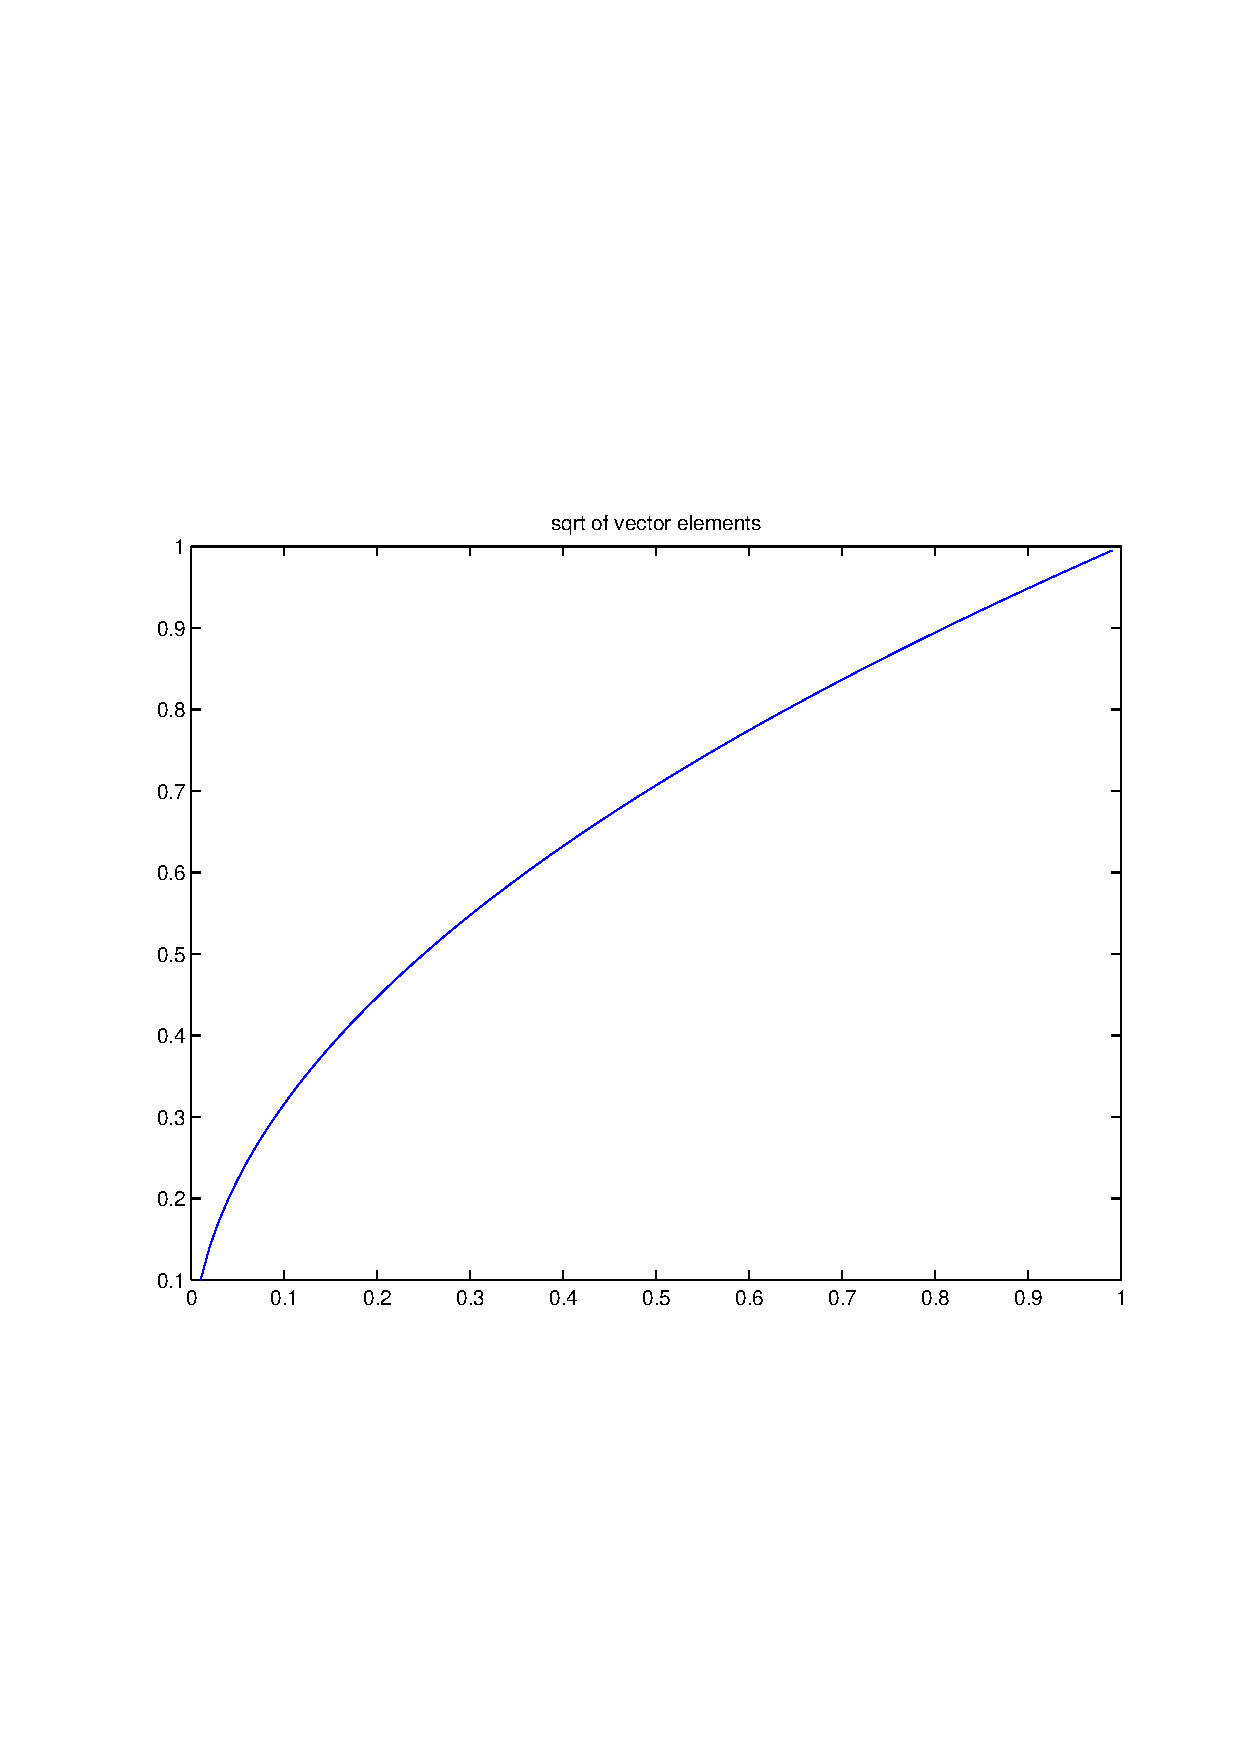
\includegraphics[width=10.0cm,height=10.0cm]{klVSLSqrt.pdf}

\includegraphics[width=10.0cm,height=10.0cm]{klVSLExp.pdf}

\includegraphics[width=10.0cm,height=10.0cm]{klVSLExpm1.pdf}

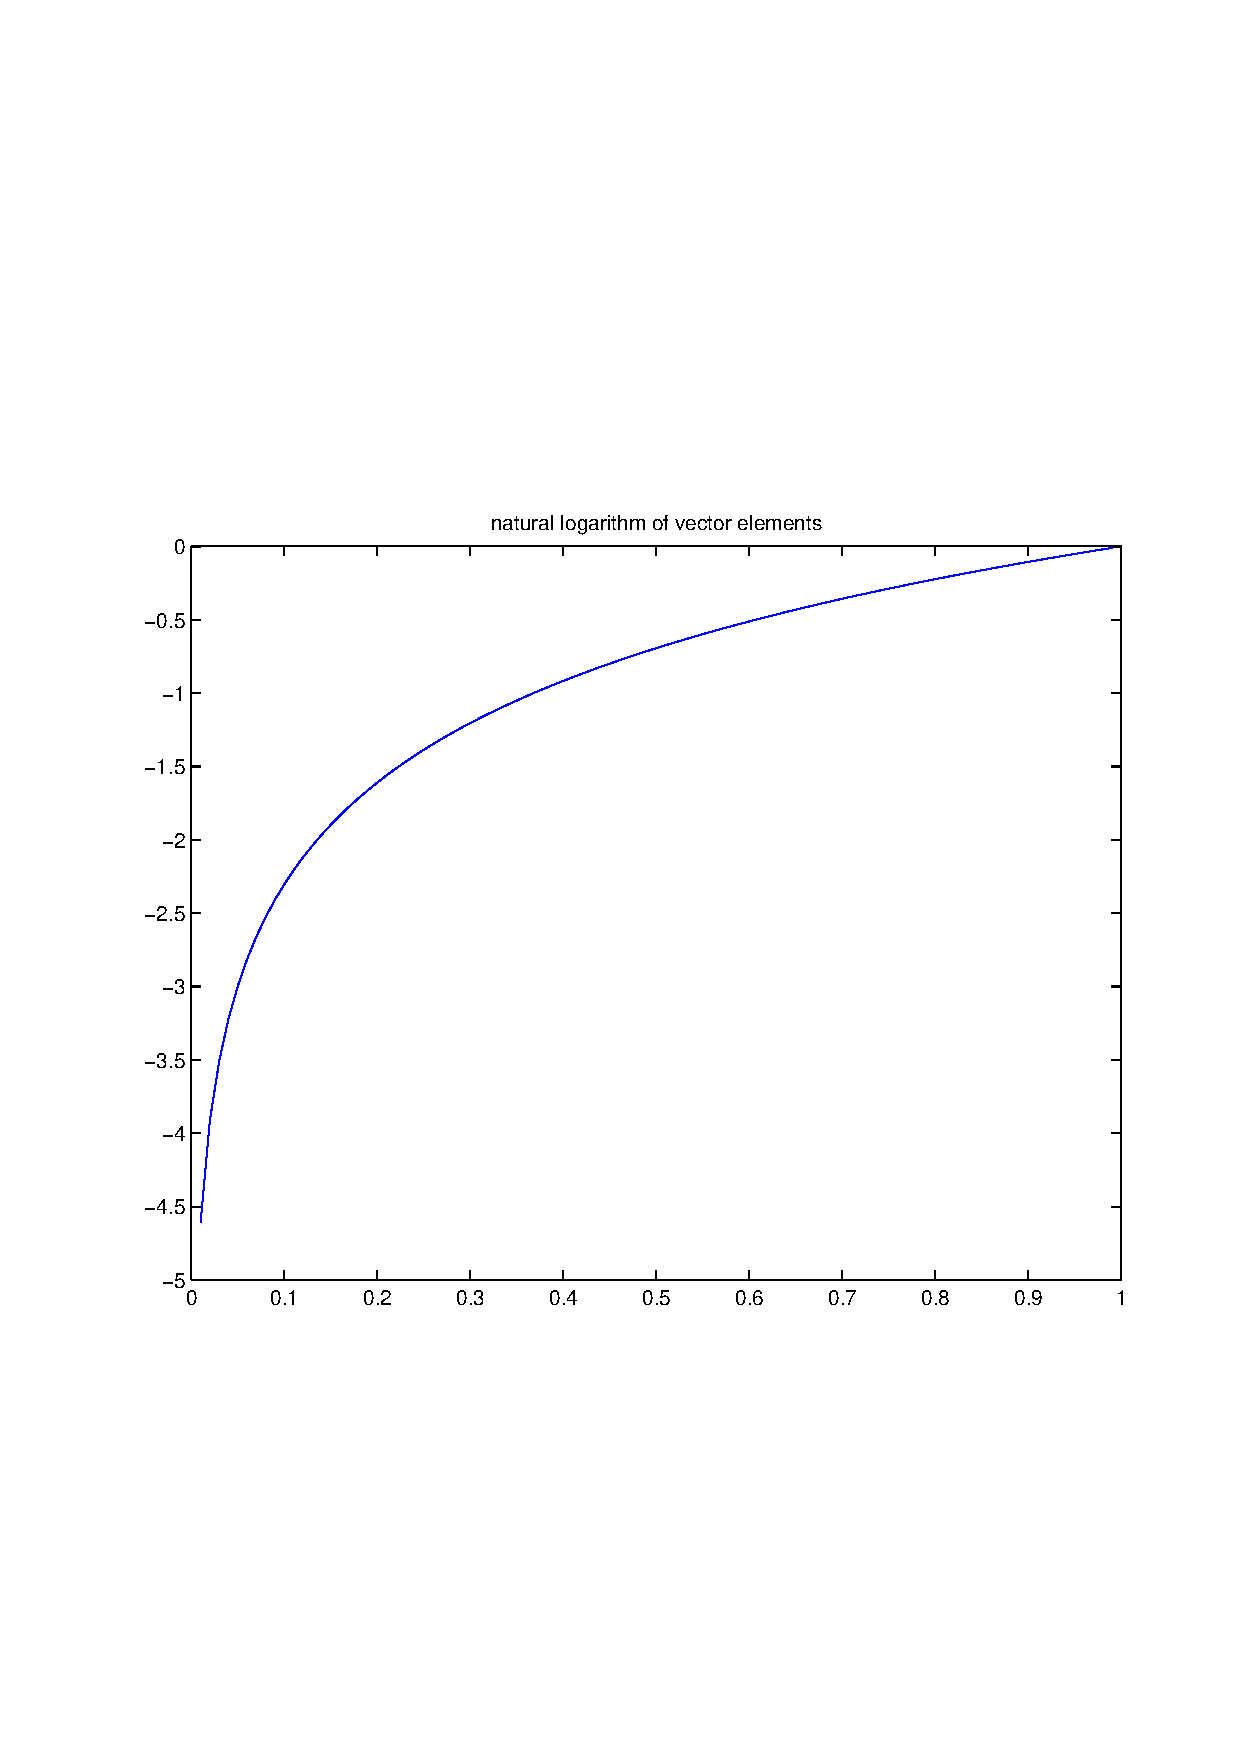
\includegraphics[width=10.0cm,height=10.0cm]{klVSLLn.pdf}

\includegraphics[width=10.0cm,height=10.0cm]{klVSLLog10.pdf}

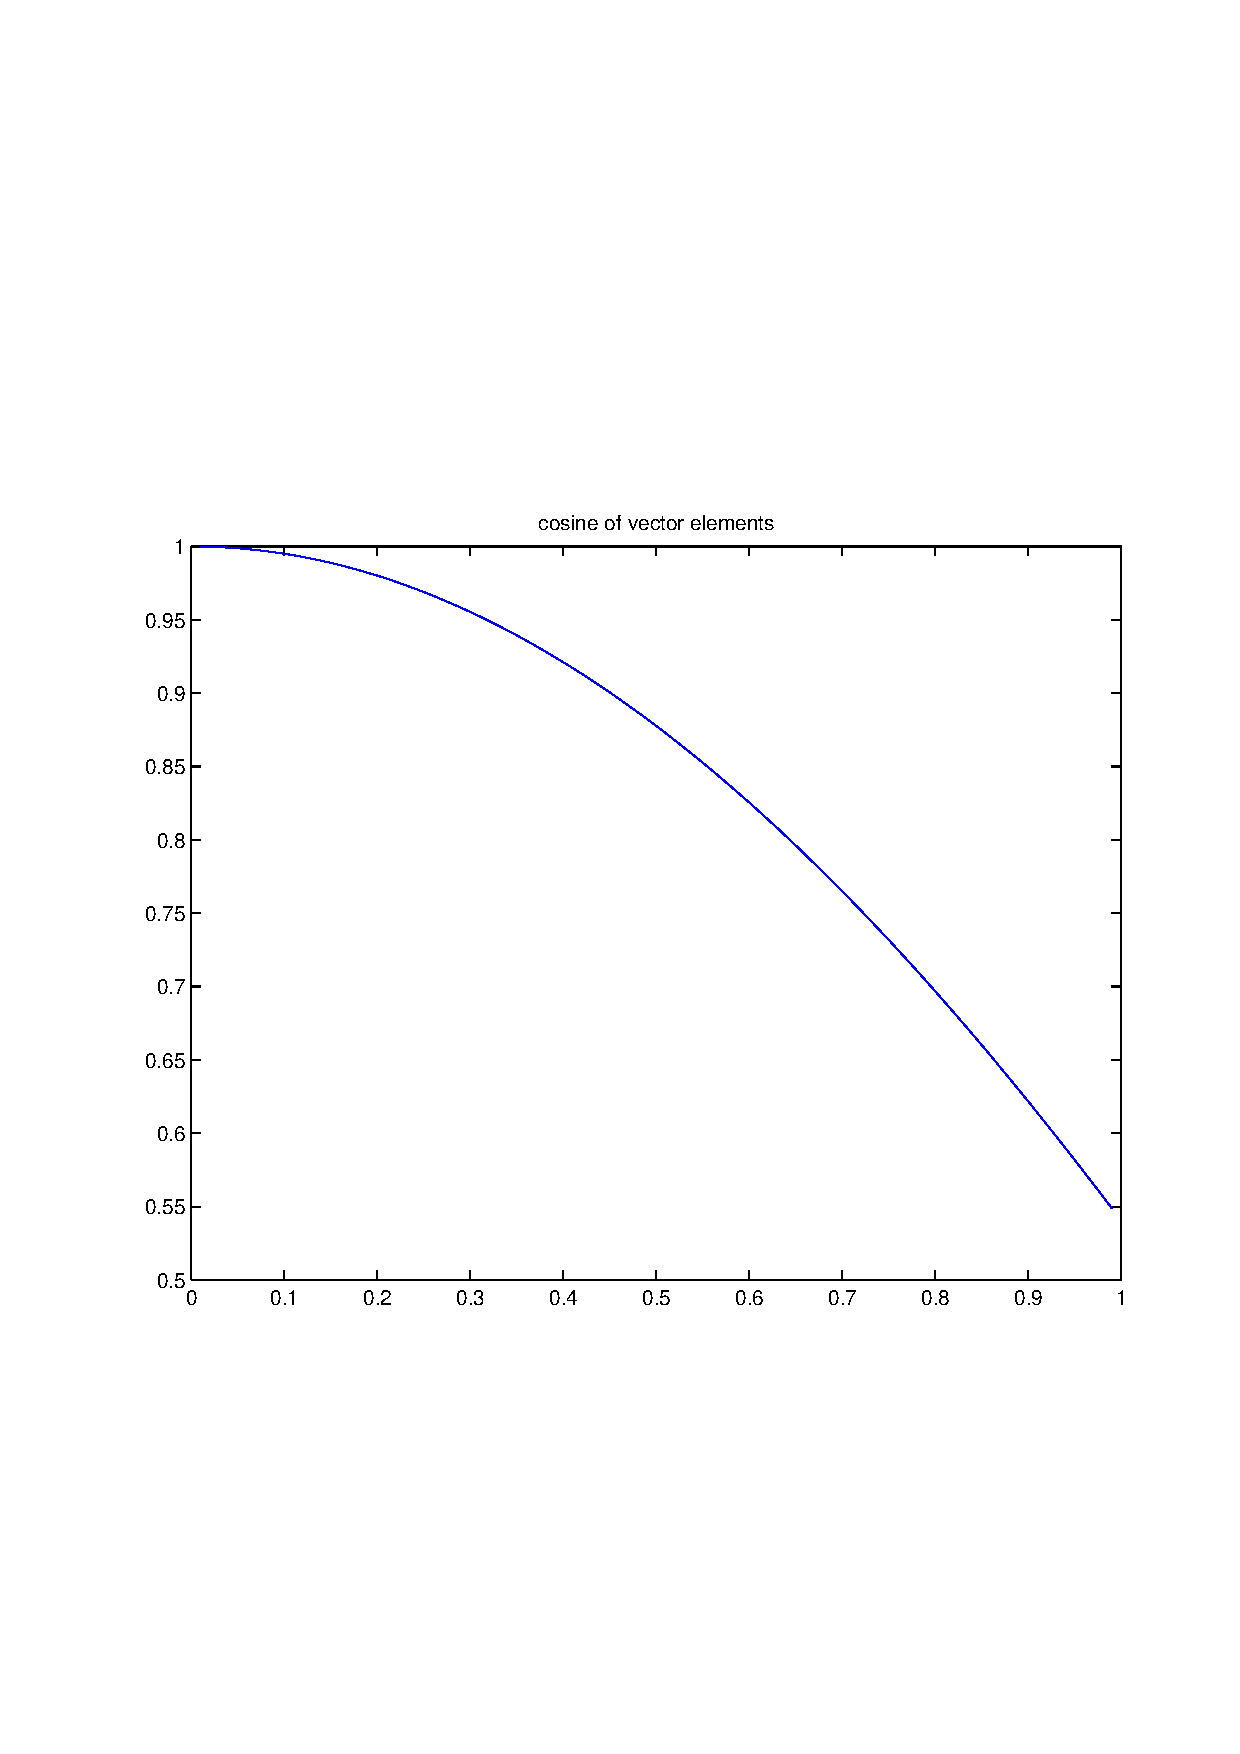
\includegraphics[width=10.0cm,height=10.0cm]{klVSLCos.pdf}

\includegraphics[width=10.0cm,height=10.0cm]{klVSLSin.pdf}

\includegraphics[width=10.0cm,height=10.0cm]{klVSLTan.pdf}

\includegraphics[width=10.0cm,height=10.0cm]{klVSLErf.pdf}

\includegraphics[width=10.0cm,height=10.0cm]{klVSLErfc.pdf}

\includegraphics[width=10.0cm,height=10.0cm]{klVSLCdfNorm.pdf}

\includegraphics[width=10.0cm,height=10.0cm]{klVSLErfInv.pdf}

\includegraphics[width=10.0cm,height=10.0cm]{klVSLLGamma.pdf}

\includegraphics[width=10.0cm,height=10.0cm]{klVSLTGamma.pdf}

QueryPerformanceCounter  =  14.6092
\subsubsection{Gram Matrix Consistency Check}
Sample Size = 4096
Feature dim = 3

$$Sigma$ = \left(
\begin{array}{
ccc}
+1.140 & +1.535 & +0.581 \\
+1.535 & +9.988 & +1.605 \\
+0.581 & +1.605 & +0.428 \\
\end{array}
\right)$ \newline 

$Sample Covariance = \left(
\begin{array}{
ccc}
+1.140 & +1.544 & +0.579 \\
+1.544 & +10.000 & +1.603 \\
+0.579 & +1.603 & +0.425 \\
\end{array}
\right)$ \newline 

$Sample Mean = \left(
\begin{array}{
ccc}
+1.00515 & +1.04349 & +1.00584 \\
\end{array}
\right)$ \newline 

$Sample Covariance-$Omega$ = \left(
\begin{array}{
ccc}
+0.000 & +0.009 & -0.003 \\
+0.009 & +0.012 & -0.002 \\
-0.003 & -0.002 & -0.003 \\
\end{array}
\right)$ \newline 

$Sample Covariance Eigs = \left(
\begin{array}{
ccc}
(+10.54001,+0.00000) & (+0.98543,+0.00000) & (+0.04026,+0.00000) \\
\end{array}
\right)$ \newline 

$Centered Mean = \left(
\begin{array}{
ccc}
+0.00000 & +0.00000 & +0.00000 \\
\end{array}
\right)$ \newline 

$Centered Covariance = \left(
\begin{array}{
ccc}
+1.140 & +1.544 & +0.579 \\
+1.544 & +10.000 & +1.603 \\
+0.579 & +1.603 & +0.425 \\
\end{array}
\right)$ \newline 

$Gram Matrix Gf Not scaled by sample size = \left(
\begin{array}{
ccc}
+4670.467 & +6321.346 & +2370.183 \\
+6321.346 & +40961.533 & +6564.912 \\
+2370.183 & +6564.912 & +1741.088 \\
\end{array}
\right)$ \newline 

$Gram Matrix Gf  scaled by sample size = \left(
\begin{array}{
ccc}
+1.140 & +1.543 & +0.579 \\
+1.543 & +10.000 & +1.603 \\
+0.579 & +1.603 & +0.425 \\
\end{array}
\right)$ \newline 

$SampleCovariance - Scaled Gf = \left(
\begin{array}{
ccc}
+0.000 & +0.000 & +0.000 \\
+0.000 & +0.002 & +0.000 \\
+0.000 & +0.000 & +0.000 \\
\end{array}
\right)$ \newline 

$EigenDecomp of SampleCovariance = \left(
\begin{array}{
ccc}
-0.170 & -0.972 & -0.164 \\
+0.919 & -0.216 & +0.331 \\
-0.357 & -0.094 & +0.929 \\
\end{array}
\right)$ \newline 

$EigenDecomp of Gram Matrix = \left(
\begin{array}{
ccc}
-0.117 & -0.976 & -0.187 \\
-0.311 & +0.214 & -0.926 \\
+0.943 & -0.050 & -0.328 \\
\end{array}
\right)$ \newline 

QueryPerformanceCounter  =  +2.108
\subsubsection{Eigen Solver Checks}
\subsubsection{Haar Distributed Random Orthogonal Matrix $A \in O(n)$}
 Testing Operator Norm
Number of Dimensions: 8

$A = \left(
\begin{array}{
cccccccc}
+0.337 & -0.370 & +0.051 & -0.683 & +0.452 & -0.235 & +0.106 & +0.098 \\
-0.319 & +0.085 & +0.030 & -0.126 & +0.475 & +0.775 & +0.213 & -0.044 \\
-0.446 & -0.041 & +0.029 & +0.360 & +0.478 & -0.426 & +0.142 & +0.488 \\
-0.394 & -0.321 & +0.509 & +0.021 & +0.103 & -0.177 & -0.234 & -0.621 \\
-0.276 & -0.585 & -0.707 & +0.032 & -0.136 & +0.011 & +0.163 & -0.188 \\
-0.272 & -0.030 & -0.154 & -0.270 & -0.026 & +0.119 & -0.839 & +0.331 \\
-0.206 & -0.396 & +0.444 & -0.152 & -0.517 & +0.185 & +0.270 & +0.454 \\
-0.487 & +0.502 & -0.123 & -0.539 & -0.209 & -0.287 & +0.255 & -0.118 \\
\end{array}
\right)$ \newline 

$Det(A) :   A \in O(n)$ = (-1.000,-0.000)

$L = \left(
\begin{array}{
cccccccc}
+1.000 & +0.000 & +0.000 & +0.000 & +0.000 & +0.000 & +0.000 & +0.000 \\
+0.567 & +1.000 & +0.000 & +0.000 & +0.000 & +0.000 & +0.000 & +0.000 \\
+0.809 & +0.836 & +1.000 & +0.000 & +0.000 & +0.000 & +0.000 & +0.000 \\
-0.692 & +0.027 & -0.015 & +1.000 & +0.000 & +0.000 & +0.000 & +0.000 \\
+0.422 & +0.698 & +0.825 & +0.287 & +1.000 & +0.000 & +0.000 & +0.000 \\
+0.654 & +0.280 & +0.253 & -0.082 & -0.767 & +1.000 & +0.000 & +0.000 \\
+0.558 & +0.357 & +0.124 & +0.105 & -0.038 & +0.242 & +1.000 & +0.000 \\
+0.915 & +0.576 & +0.446 & -0.546 & -0.972 & -0.074 & -0.677 & +1.000 \\
\end{array}
\right)$ \newline 

$U = \left(
\begin{array}{
cccccccc}
-0.487 & +0.502 & -0.123 & -0.539 & -0.209 & -0.287 & +0.255 & -0.118 \\
+0.000 & -0.869 & -0.638 & +0.338 & -0.017 & +0.174 & +0.018 & -0.121 \\
+0.000 & +0.000 & +1.142 & +0.175 & +0.287 & -0.091 & -0.455 & -0.424 \\
+0.000 & +0.000 & +0.000 & -1.062 & +0.312 & -0.439 & +0.275 & +0.014 \\
+0.000 & +0.000 & +0.000 & +0.000 & -0.743 & +0.385 & +0.446 & +0.934 \\
+0.000 & +0.000 & +0.000 & +0.000 & +0.000 & +1.196 & +0.521 & +0.892 \\
+0.000 & +0.000 & +0.000 & +0.000 & +0.000 & +0.000 & -1.069 & +0.311 \\
+0.000 & +0.000 & +0.000 & +0.000 & +0.000 & +0.000 & +0.000 & +2.047 \\
\end{array}
\right)$ \newline 

$L * U  = \left(
\begin{array}{
cccccccc}
-0.487 & +0.502 & -0.123 & -0.539 & -0.209 & -0.287 & +0.255 & -0.118 \\
-0.276 & -0.585 & -0.707 & +0.032 & -0.136 & +0.011 & +0.163 & -0.188 \\
-0.394 & -0.321 & +0.509 & +0.021 & +0.103 & -0.177 & -0.234 & -0.621 \\
+0.337 & -0.370 & +0.051 & -0.683 & +0.452 & -0.235 & +0.106 & +0.098 \\
-0.206 & -0.396 & +0.444 & -0.152 & -0.517 & +0.185 & +0.270 & +0.454 \\
-0.319 & +0.085 & +0.030 & -0.126 & +0.475 & +0.775 & +0.213 & -0.044 \\
-0.272 & -0.030 & -0.154 & -0.270 & -0.026 & +0.119 & -0.839 & +0.331 \\
-0.446 & -0.041 & +0.029 & +0.360 & +0.478 & -0.426 & +0.142 & +0.488 \\
\end{array}
\right)$ \newline 

$Det(L) :    = (+1.000,+0.000)     Det(U) :    = (-1.000,+0.000)     Det(LU) :    = (-1.000,+0.000)$

$||A||_{L_1}$  = +2.738

$||A||_{L_{\infty}}$ = +2.624

$||A^{-1}||_{L_1}$  = +2.624

$||A^{-1}||_{L_{\infty}}$ = +2.738

$||A||_{L_{\infty}} * ||A^{-1}||_{L_{\infty}} = +7.183$

$||A||_{L_1} * ||A^{-1}||_{L_1} = +7.183$

Frobenious Norm  $||A||_{\textit{F}}$ via $\sum\limits_{i,j =0}^{n} \|A_{i,j}|$   of  $A \in O(n)$  +2.828

$L_1$ condition number of Haar Distributed Random Orthogonal Matrix $A \in O(n)$ +6.601

$A = \left(
\begin{array}{
cccccccc}
+0.337 & -0.370 & +0.051 & -0.683 & +0.452 & -0.235 & +0.106 & +0.098 \\
-0.319 & +0.085 & +0.030 & -0.126 & +0.475 & +0.775 & +0.213 & -0.044 \\
-0.446 & -0.041 & +0.029 & +0.360 & +0.478 & -0.426 & +0.142 & +0.488 \\
-0.394 & -0.321 & +0.509 & +0.021 & +0.103 & -0.177 & -0.234 & -0.621 \\
-0.276 & -0.585 & -0.707 & +0.032 & -0.136 & +0.011 & +0.163 & -0.188 \\
-0.272 & -0.030 & -0.154 & -0.270 & -0.026 & +0.119 & -0.839 & +0.331 \\
-0.206 & -0.396 & +0.444 & -0.152 & -0.517 & +0.185 & +0.270 & +0.454 \\
-0.487 & +0.502 & -0.123 & -0.539 & -0.209 & -0.287 & +0.255 & -0.118 \\
\end{array}
\right)$ \newline 

$L_{\infty}$ condition number of Haar Distributed Random Orthogonal Matrix $A \in O(n)$ +5.727

Eigenvalues of $A \in O(n)$

(-1.000,+0.000), (-0.409,+0.912), (-0.409,-0.912), (-0.213,+0.977), (-0.213,-0.977), (+0.926,+0.377), (+0.926,-0.377), (+1.000,+0.000)

 $|\lambda | : \lambda \in \sigma(A) , A \in O(n)$

+1.000, +1.000, +1.000, +1.000, +1.000, +1.000, +1.000, +1.000


Calculating $A^{\dag} A,$  we expect $A^{\dag} A \approx I$

$A^{\dag} A = \left(
\begin{array}{
cccccccc}
+1.000 & +0.000 & -0.000 & -0.000 & +0.000 & -0.000 & -0.000 & -0.000 \\
+0.000 & +1.000 & +0.000 & +0.000 & +0.000 & -0.000 & -0.000 & -0.000 \\
-0.000 & +0.000 & +1.000 & +0.000 & -0.000 & -0.000 & +0.000 & +0.000 \\
-0.000 & +0.000 & +0.000 & +1.000 & -0.000 & -0.000 & -0.000 & +0.000 \\
+0.000 & +0.000 & -0.000 & -0.000 & +1.000 & -0.000 & -0.000 & -0.000 \\
-0.000 & -0.000 & -0.000 & -0.000 & -0.000 & +1.000 & -0.000 & +0.000 \\
-0.000 & -0.000 & +0.000 & -0.000 & -0.000 & -0.000 & +1.000 & +0.000 \\
-0.000 & -0.000 & +0.000 & +0.000 & -0.000 & +0.000 & +0.000 & +1.000 \\
\end{array}
\right)$ \newline 

Calculating $A^{-1} ,  A \in O(n)$.

$A^{-1} = \left(
\begin{array}{
cccccccc}
+0.337 & -0.319 & -0.446 & -0.394 & -0.276 & -0.272 & -0.206 & -0.487 \\
-0.370 & +0.085 & -0.041 & -0.321 & -0.585 & -0.030 & -0.396 & +0.502 \\
+0.051 & +0.030 & +0.029 & +0.509 & -0.707 & -0.154 & +0.444 & -0.123 \\
-0.683 & -0.126 & +0.360 & +0.021 & +0.032 & -0.270 & -0.152 & -0.539 \\
+0.452 & +0.475 & +0.478 & +0.103 & -0.136 & -0.026 & -0.517 & -0.209 \\
-0.235 & +0.775 & -0.426 & -0.177 & +0.011 & +0.119 & +0.185 & -0.287 \\
+0.106 & +0.213 & +0.142 & -0.234 & +0.163 & -0.839 & +0.270 & +0.255 \\
+0.098 & -0.044 & +0.488 & -0.621 & -0.188 & +0.331 & +0.454 & -0.118 \\
\end{array}
\right)$ \newline 

Calculating $A^{-1} *A  ,  A \in O(n)$.   We expect $A^{-1} *A  \approx I$. 

$A^{-1} *A = \left(
\begin{array}{
cccccccc}
+1.000 & +0.000 & +0.000 & +0.000 & -0.000 & -0.000 & -0.000 & -0.000 \\
+0.000 & +1.000 & +0.000 & +0.000 & -0.000 & +0.000 & -0.000 & -0.000 \\
+0.000 & +0.000 & +1.000 & -0.000 & -0.000 & +0.000 & +0.000 & +0.000 \\
+0.000 & +0.000 & +0.000 & +1.000 & +0.000 & -0.000 & +0.000 & -0.000 \\
+0.000 & -0.000 & +0.000 & +0.000 & +1.000 & +0.000 & +0.000 & +0.000 \\
-0.000 & +0.000 & -0.000 & -0.000 & +0.000 & +1.000 & +0.000 & -0.000 \\
+0.000 & +0.000 & +0.000 & +0.000 & -0.000 & +0.000 & +1.000 & +0.000 \\
-0.000 & +0.000 & +0.000 & -0.000 & +0.000 & +0.000 & -0.000 & +1.000 \\
\end{array}
\right)$ \newline 

Calculating SVD of  $A \in O(n)$

$U = \left(
\begin{array}{
cccccccc}
-0.197 & +0.270 & +0.429 & +0.066 & +0.151 & -0.044 & +0.361 & +0.738 \\
-0.014 & -0.610 & +0.316 & +0.129 & +0.034 & +0.689 & -0.139 & +0.126 \\
-0.199 & +0.500 & -0.018 & -0.172 & +0.624 & +0.420 & -0.293 & -0.170 \\
-0.337 & +0.370 & -0.051 & +0.683 & -0.452 & +0.235 & -0.106 & -0.098 \\
+0.403 & +0.336 & +0.035 & -0.432 & -0.523 & +0.280 & -0.323 & +0.284 \\
-0.070 & -0.124 & -0.840 & +0.046 & +0.096 & +0.185 & +0.054 & +0.475 \\
-0.151 & -0.151 & +0.080 & +0.147 & +0.106 & -0.423 & -0.804 & +0.301 \\
-0.786 & -0.130 & -0.009 & -0.522 & -0.299 & -0.000 & +0.015 & -0.056 \\
\end{array}
\right)$ \newline 

$S = \left(
\begin{array}{
cccccccc}
+1.000 & +0.000 & +0.000 & +0.000 & +0.000 & +0.000 & +0.000 & +0.000 \\
+0.000 & +1.000 & +0.000 & +0.000 & +0.000 & +0.000 & +0.000 & +0.000 \\
+0.000 & +0.000 & +1.000 & +0.000 & +0.000 & +0.000 & +0.000 & +0.000 \\
+0.000 & +0.000 & +0.000 & +1.000 & +0.000 & +0.000 & +0.000 & +0.000 \\
+0.000 & +0.000 & +0.000 & +0.000 & +1.000 & +0.000 & +0.000 & +0.000 \\
+0.000 & +0.000 & +0.000 & +0.000 & +0.000 & +1.000 & +0.000 & +0.000 \\
+0.000 & +0.000 & +0.000 & +0.000 & +0.000 & +0.000 & +1.000 & +0.000 \\
+0.000 & +0.000 & +0.000 & +0.000 & +0.000 & +0.000 & +0.000 & +1.000 \\
\end{array}
\right)$ \newline 

$V = \left(
\begin{array}{
cccccccc}
+0.000 & -0.000 & +0.000 & -1.000 & -0.000 & -0.000 & -0.000 & -0.000 \\
+0.173 & +0.462 & +0.694 & -0.000 & -0.157 & +0.160 & -0.443 & +0.168 \\
+0.615 & -0.148 & +0.000 & -0.000 & -0.625 & +0.235 & +0.392 & -0.000 \\
-0.309 & +0.201 & +0.069 & -0.000 & -0.462 & -0.690 & +0.238 & +0.337 \\
-0.506 & +0.098 & -0.326 & -0.000 & -0.378 & +0.596 & -0.129 & +0.337 \\
-0.107 & +0.178 & +0.311 & +0.000 & +0.404 & +0.271 & +0.714 & +0.337 \\
+0.460 & +0.495 & -0.540 & +0.000 & +0.230 & -0.102 & -0.109 & +0.421 \\
+0.130 & -0.662 & +0.137 & +0.000 & +0.114 & -0.065 & -0.233 & +0.674 \\
\end{array}
\right)$ \newline 

$U S V = \left(
\begin{array}{
cccccccc}
+0.481 & -0.229 & +0.036 & +0.197 & -0.248 & +0.092 & -0.198 & +0.753 \\
-0.089 & -0.329 & -0.119 & +0.014 & +0.086 & +0.101 & +0.899 & +0.211 \\
-0.388 & +0.302 & +0.398 & +0.199 & -0.141 & +0.721 & +0.022 & +0.140 \\
-0.037 & +0.326 & +0.568 & +0.337 & -0.112 & -0.612 & +0.239 & +0.108 \\
+0.336 & -0.286 & +0.675 & -0.403 & +0.393 & +0.139 & -0.002 & -0.116 \\
-0.534 & -0.169 & -0.020 & +0.070 & +0.628 & -0.178 & -0.260 & +0.432 \\
-0.361 & -0.714 & +0.214 & +0.151 & -0.455 & -0.096 & -0.165 & -0.218 \\
+0.284 & -0.148 & -0.044 & +0.786 & +0.377 & +0.161 & -0.021 & -0.330 \\
\end{array}
\right)$ \newline 

Calculating first few eigenvectors of $A \in O(n)$ using LAPACK syevx

\subsubsection{Wishart Matrix $A \in W(n)$}
$L_1$ condition number of Wishart Matrix +1489.694
$L_infty$ condition number of Wishart Matrix +1489.694
\subsubsection{Gaussian Orthogonal Ensemble $A \in GOE(n)$}
$L_1$ condition number of GOE Matrix +66.900
$L_\infty$ condition number of GOE Matrix +66.900
\subsubsection{The Identity Matrix $I \in M(n)$}
$L_1$ condition number of $I$ = +1.000
$L_\infty$ condition number of $I$ = +1.000
QueryPerformanceCounter  =  +0.225
\subsubsection{Generate Tracey Widom Sample}
\subsubsection{Sample from $W_n m$ times and calculate empirical PDF of the first eig}
Here we generate histograms of $\lambda_1$ for GOE (Gaussian Orthogonal Ensemble), and W (Wishart) 		 distributed of random matrices
These should approximate the celebrated Tracy Widom distribution.
Dimension $n = 128$

Sample size $m = 32$

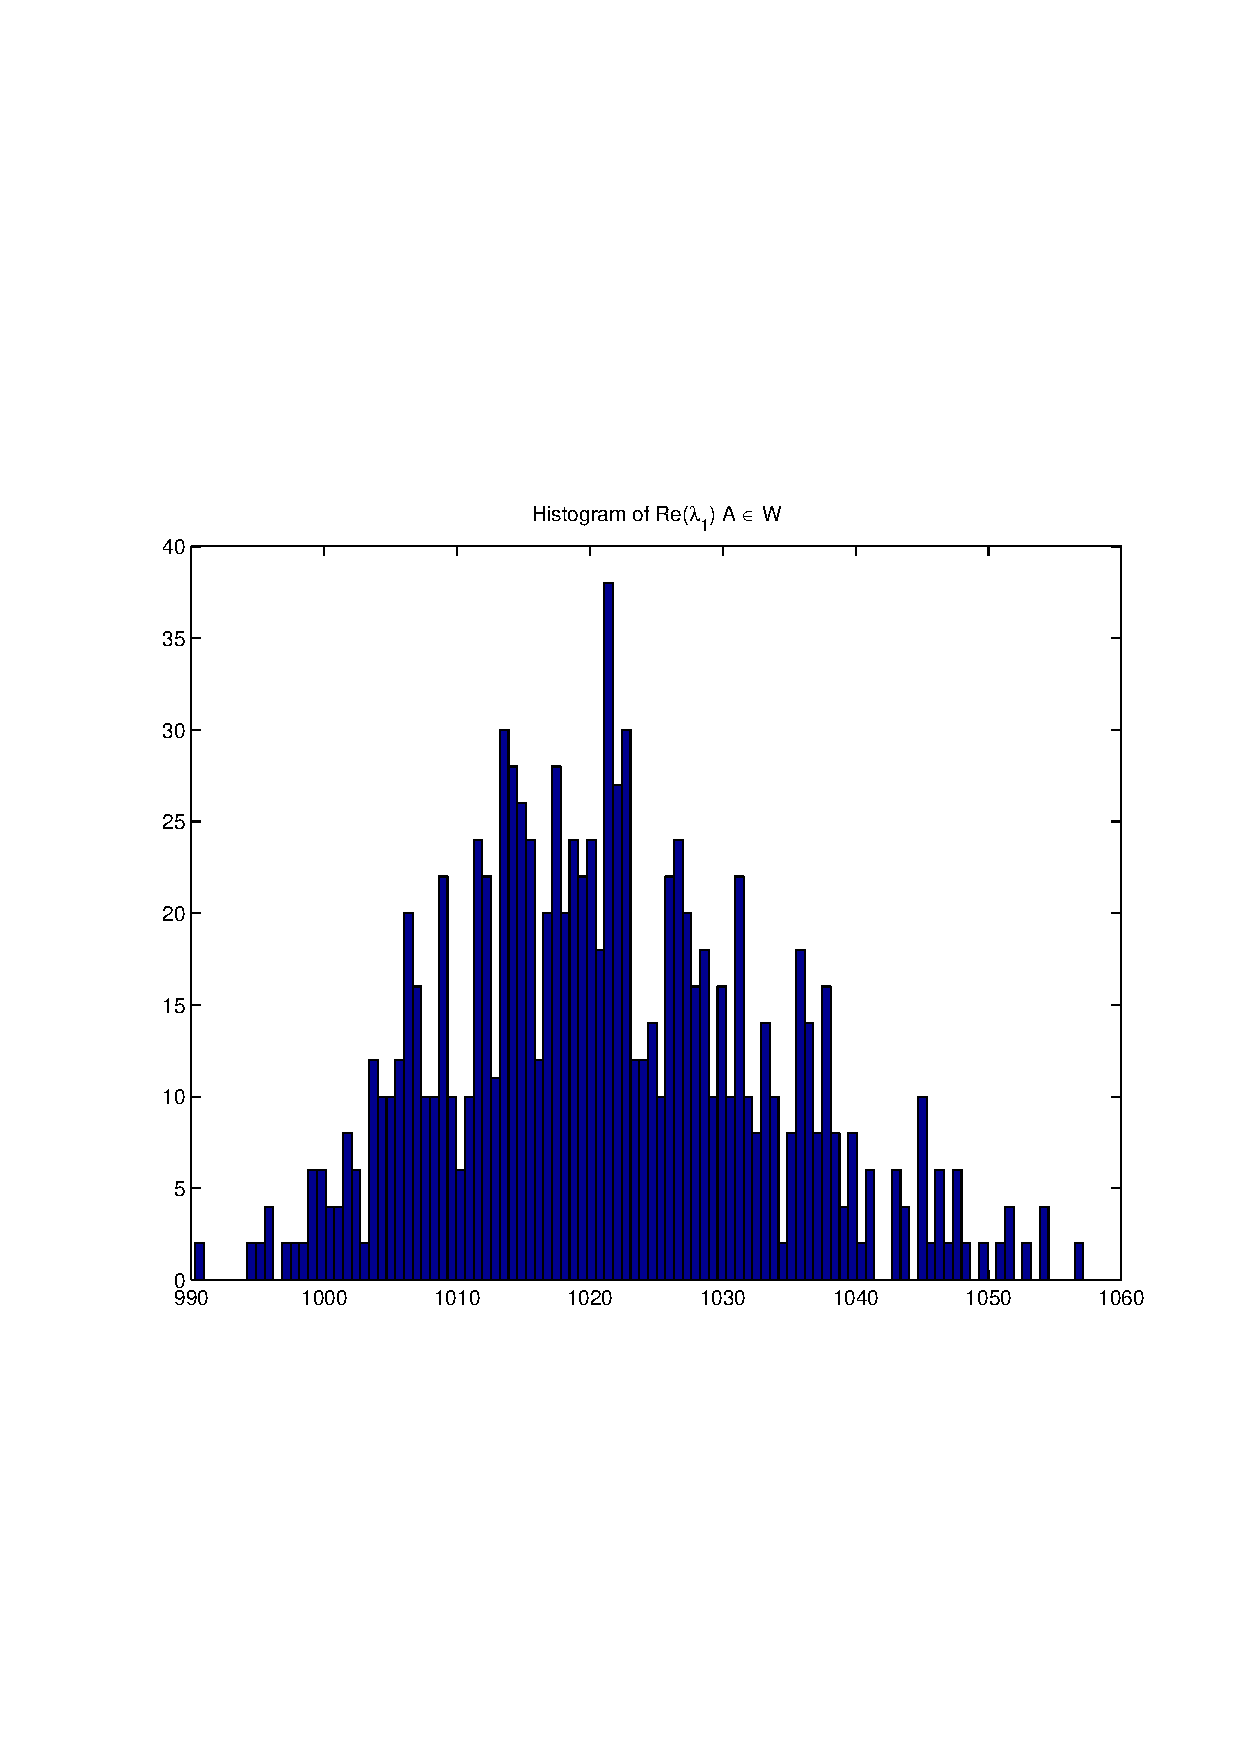
\includegraphics[width=10.0cm,height=10.0cm]{Re_TraceyWidom.pdf}

\includegraphics[width=10.0cm,height=10.0cm]{Im_TraceyWidom.pdf}

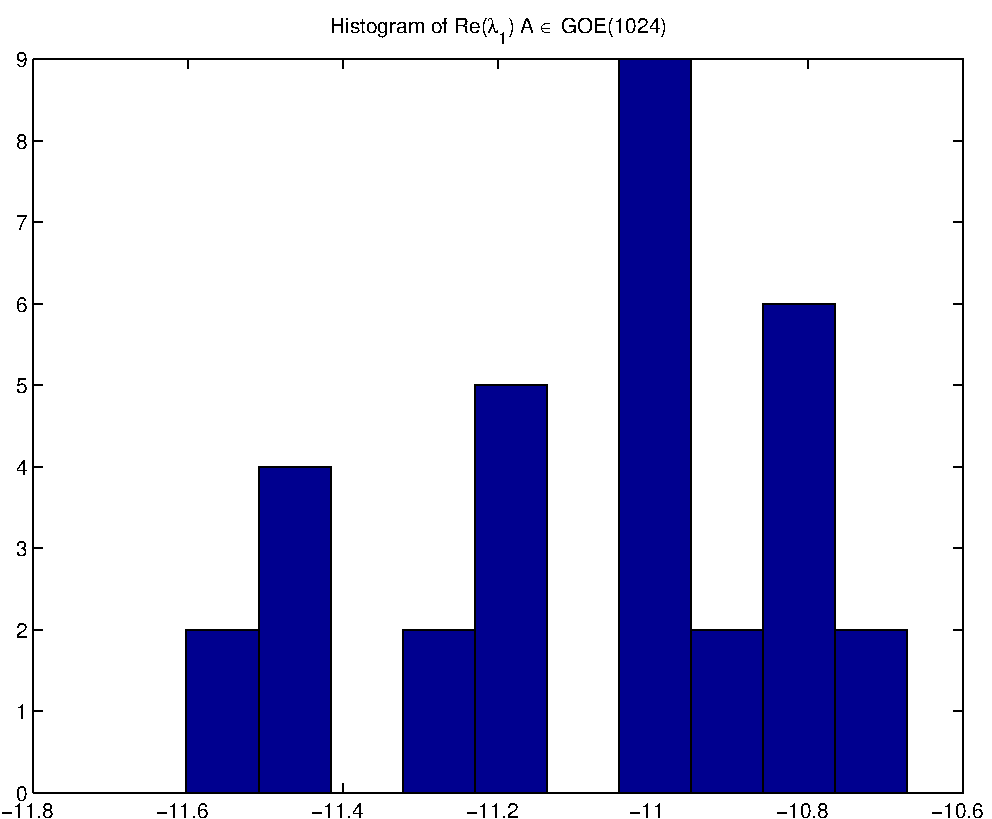
\includegraphics[width=10.0cm,height=10.0cm]{Re_Winger.pdf}

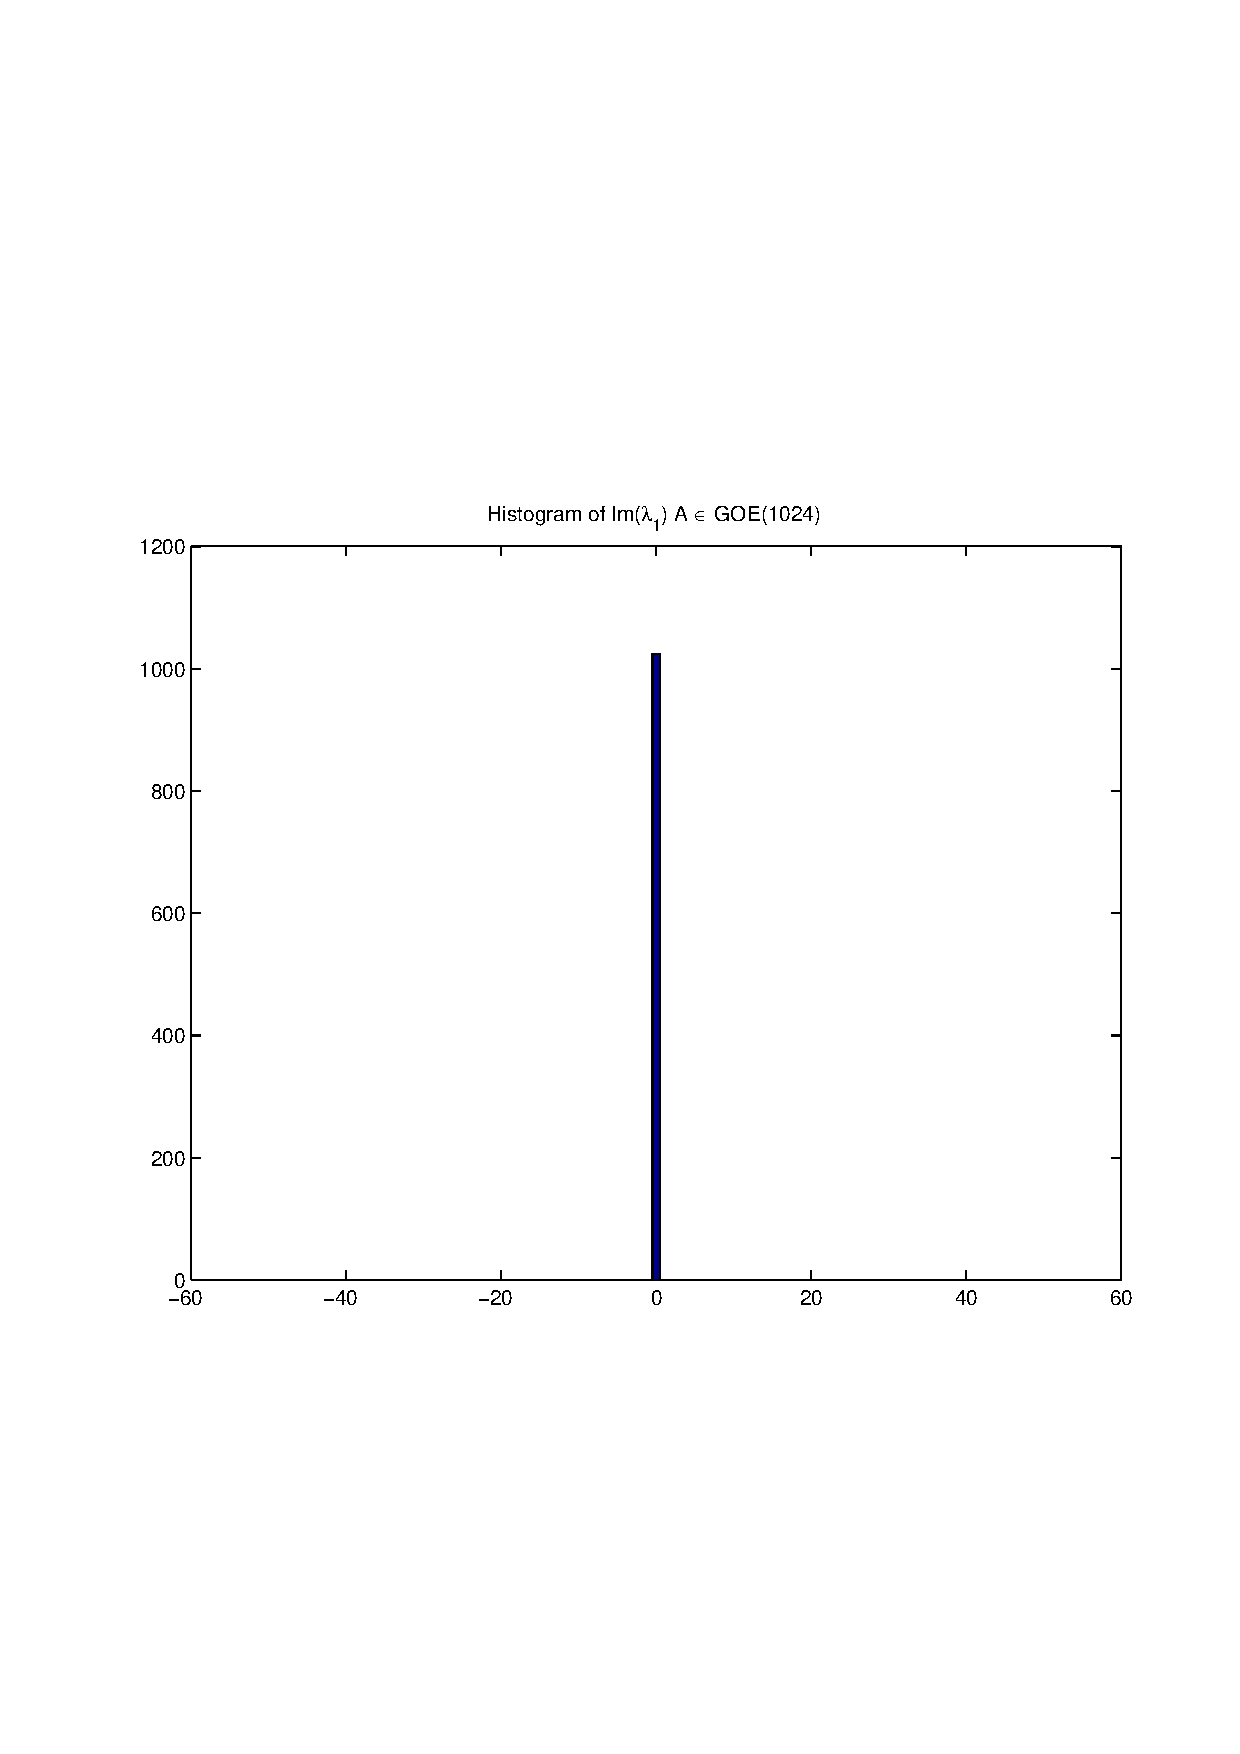
\includegraphics[width=10.0cm,height=10.0cm]{Im_Winger.pdf}

QueryPerformanceCounter  =  +4.821
\subsubsection{Approximate Winger Distribution}
\subsubsection{Verfy Winger Law.}
Let $M_n = [X_{ij} ]$ a symmetric n x n matrix with Random entries such that $X_{i,j} = X_{j,i}$, 		  and $X_{i,j}$ are iid $orall i < j,$ and $Xjj$ are iid $orall j  :  ; E[X^2_{ij} ] = 1, & E[X_{ij}] = 0$ 		  and that all moments exists for each of the entries.  		  The eigenvector of this random matrix; $ lambda_1 leq ... leq lambda_n$ depends continuously on $Mn$.
Dimension $n = 512$

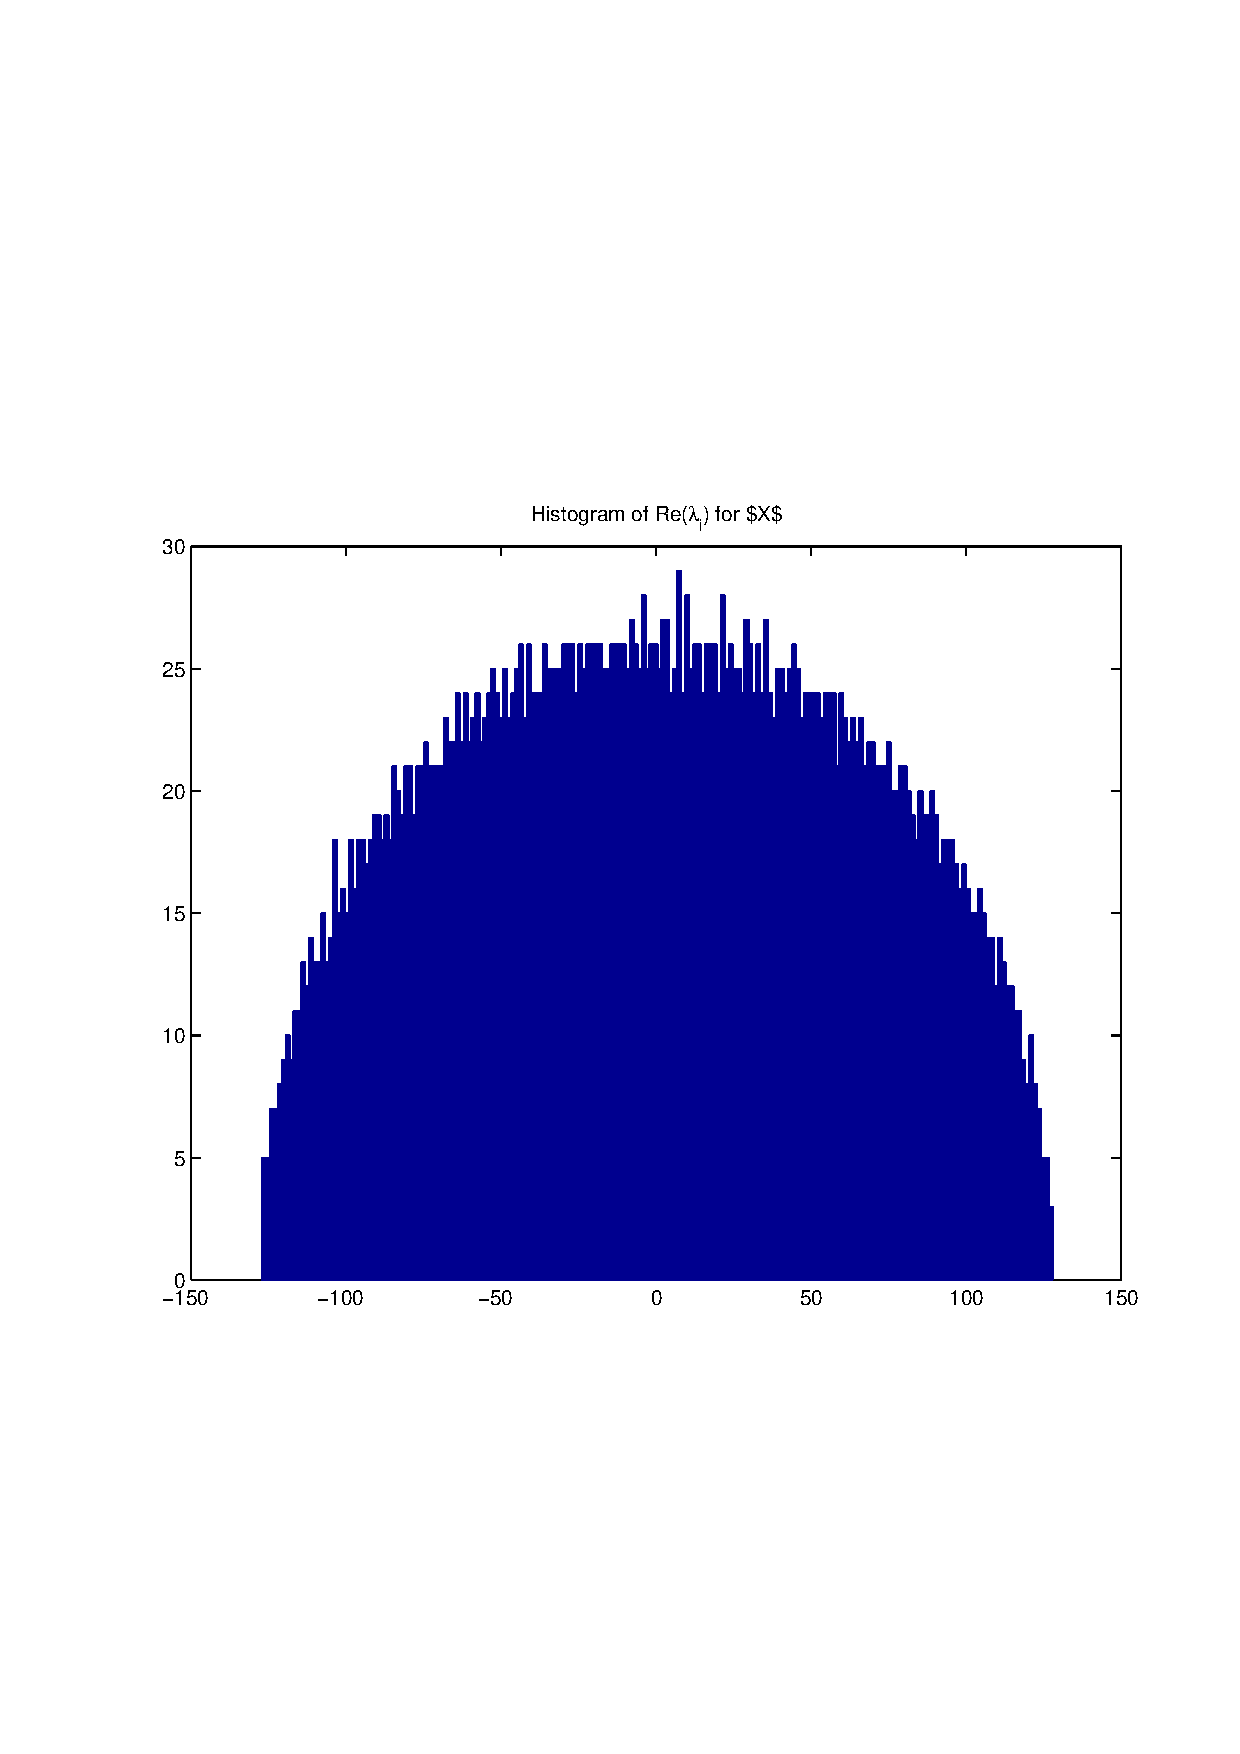
\includegraphics[width=10.0cm,height=10.0cm]{Re_lambda_n.pdf}

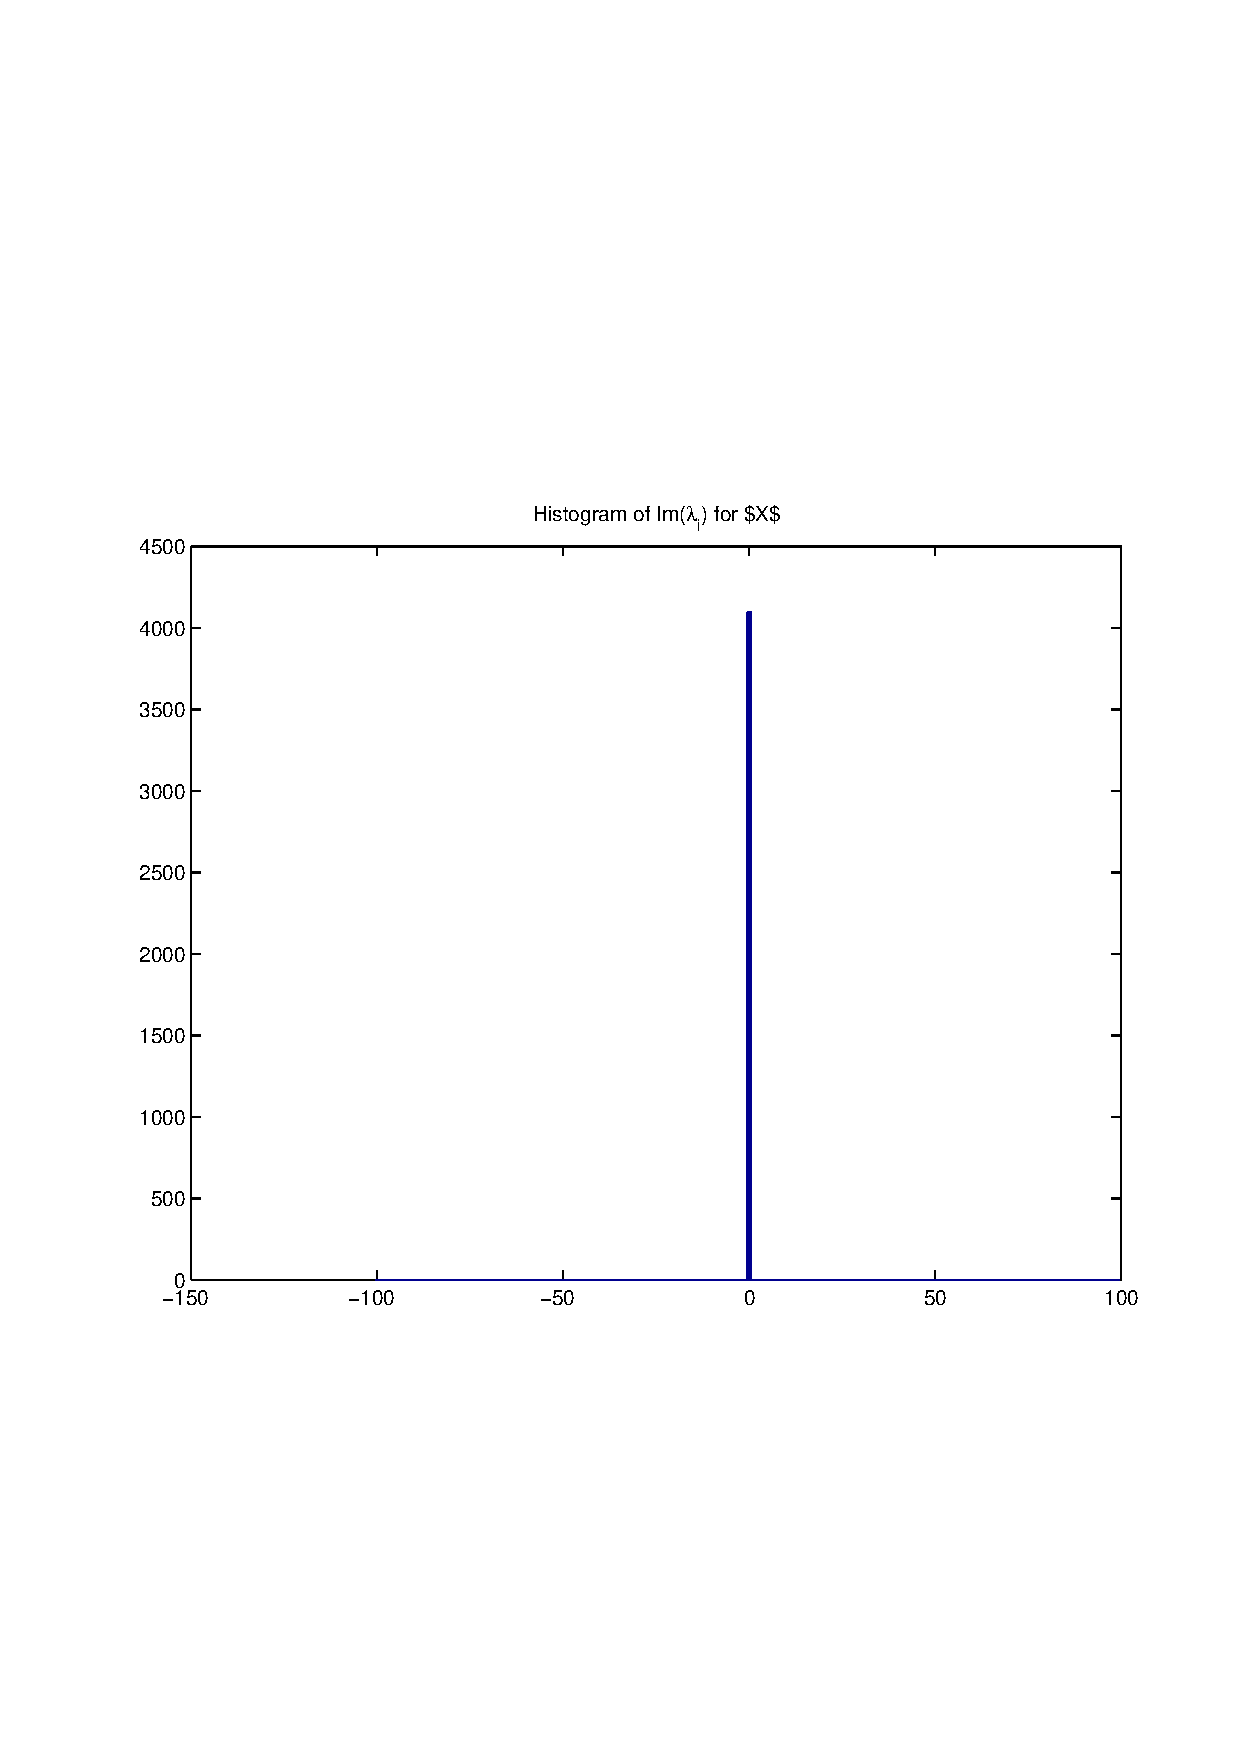
\includegraphics[width=10.0cm,height=10.0cm]{Im_lambda_n.pdf}

QueryPerformanceCounter  =  +2.568
\subsubsection{Iterated Exponential Filtering }
$\mu_1 =+0.093$
$\mu_2 =+0.726$
$\mu_3 =+0.011$
$\mu_4 =+2.178$
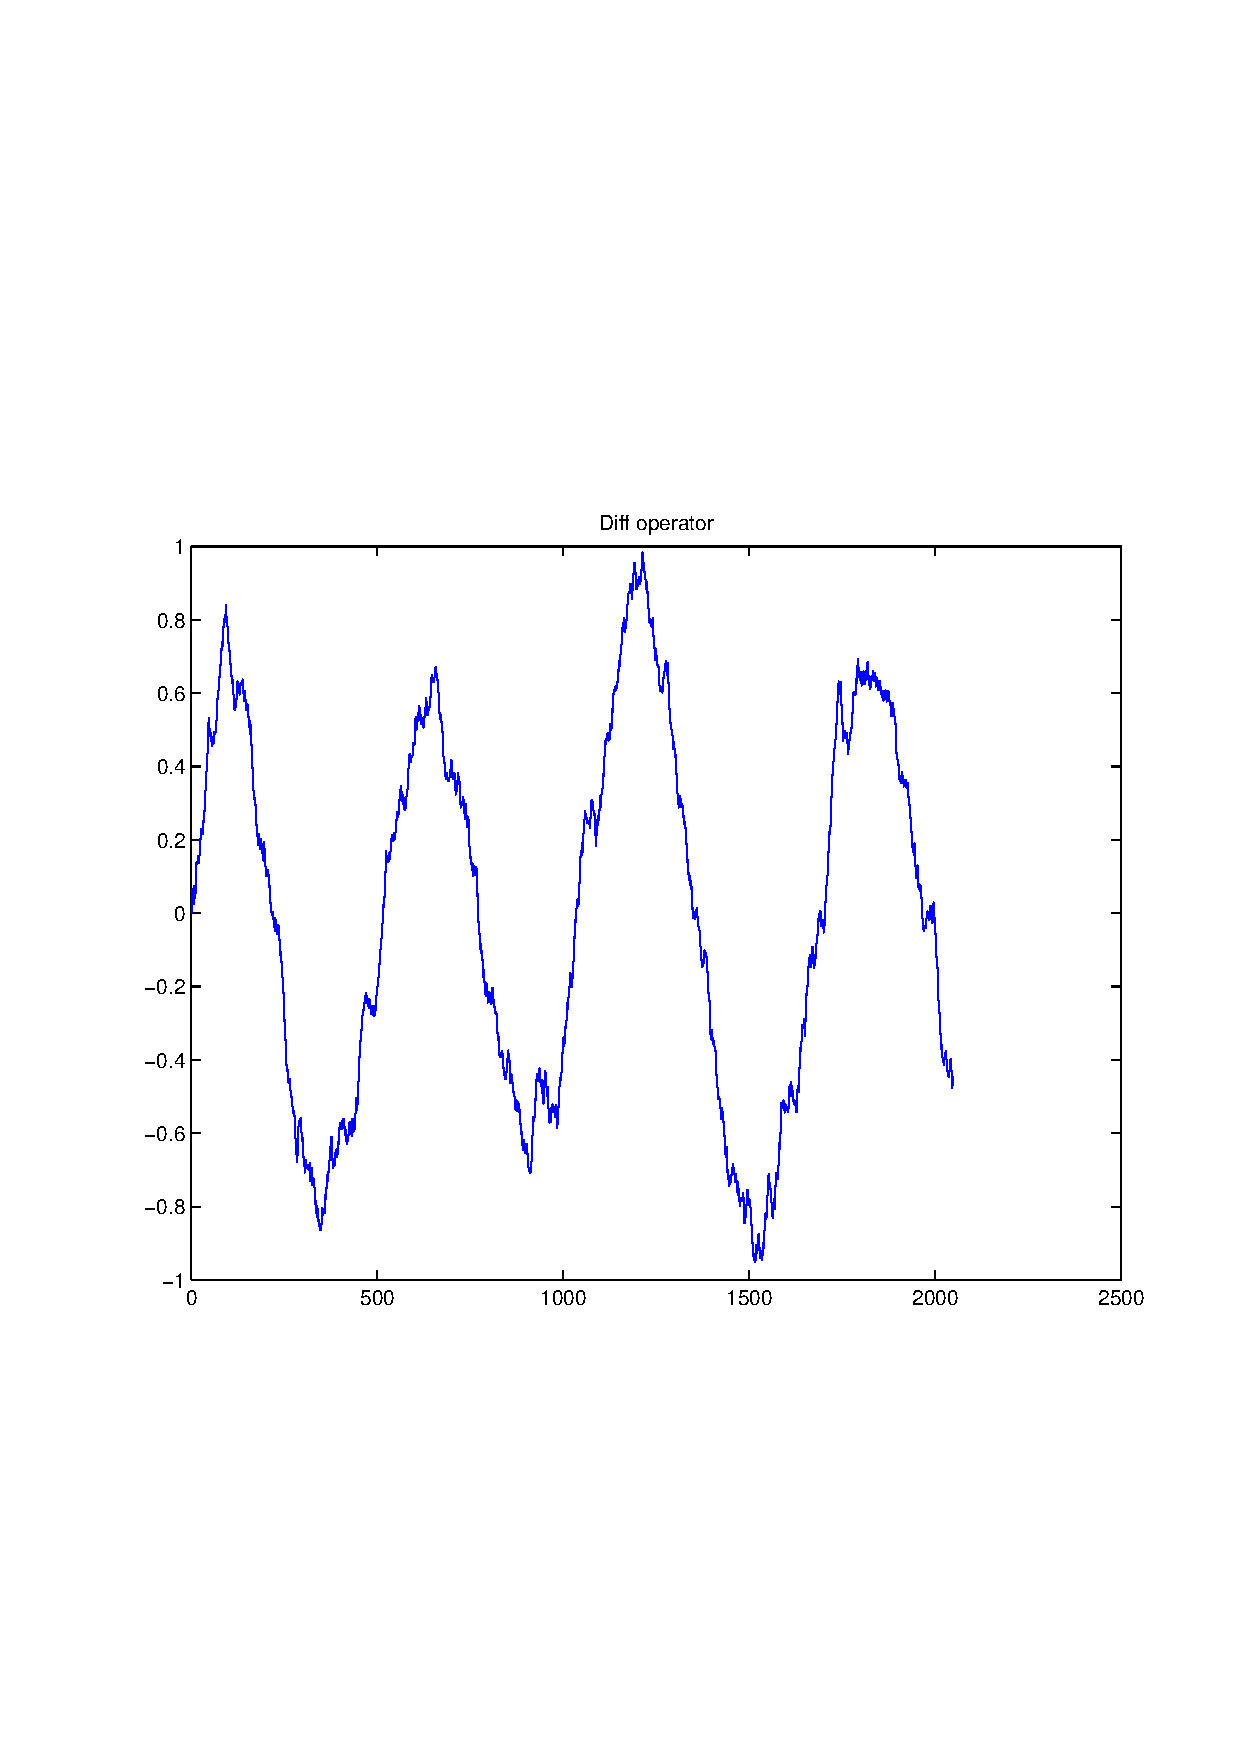
\includegraphics[width=10.0cm,height=10.0cm]{DIFF.pdf}

QueryPerformanceCounter  =  +1.367
\subsubsection{Matrix Exponential }
$SPD Matrix = \left(
\begin{array}{
cccccccc}
+10.539 & -0.499 & -0.010 & +0.368 & +0.465 & -0.492 & -0.126 & +0.437 \\
-0.499 & +7.286 & +0.365 & -0.481 & -0.337 & -0.466 & +0.279 & +0.056 \\
-0.010 & +0.365 & +6.705 & -0.205 & +0.467 & +0.131 & +0.077 & -0.089 \\
+0.368 & -0.481 & -0.205 & +6.496 & -0.402 & -0.209 & +0.043 & -0.041 \\
+0.465 & -0.337 & +0.467 & -0.402 & +4.578 & +0.272 & +0.289 & -0.285 \\
-0.492 & -0.466 & +0.131 & -0.209 & +0.272 & +8.181 & +0.343 & -0.244 \\
-0.126 & +0.279 & +0.077 & +0.043 & +0.289 & +0.343 & +5.938 & -0.212 \\
+0.437 & +0.056 & -0.089 & -0.041 & -0.285 & -0.244 & -0.212 & +9.691 \\
\end{array}
\right)$ \newline 

$SPD Eigs = \left(
\begin{array}{
cccccccc}
(+10.93611,+0.00000) & (+9.60778,+0.00000) & (+4.23666,+0.00000) & (+8.36911,+0.00000) & (+7.56229,+0.00000) & (+5.82791,+0.00000) & (+6.54198,+0.00000) & (+6.33139,+0.00000) \\
\end{array}
\right)$ \newline 

$exp(SPD) = \left(
\begin{array}{
cccccccc}
+47863.969 & -6460.093 & -1078.770 & +4706.958 & +2535.224 & -8475.398 & -2406.368 & +12977.552 \\
-6460.093 & +2780.574 & +516.920 & -1069.918 & -548.083 & -109.707 & +386.466 & -807.216 \\
-1078.770 & +516.920 & +1015.281 & -385.755 & +176.069 & +458.541 & +212.284 & -859.022 \\
+4706.958 & -1069.918 & -385.755 & +1267.210 & +111.181 & -1018.272 & -287.809 & +1036.628 \\
+2535.224 & -548.083 & +176.069 & +111.181 & +413.265 & +135.193 & +45.490 & -502.411 \\
-8475.398 & -109.707 & +458.541 & -1018.272 & +135.193 & +5613.026 & +968.003 & -4270.737 \\
-2406.368 & +386.466 & +212.284 & -287.809 & +45.490 & +968.003 & +632.432 & -1645.725 \\
+12977.552 & -807.216 & -859.022 & +1036.628 & -502.411 & -4270.737 & -1645.725 & +19362.944 \\
\end{array}
\right)$ \newline 

$exp(SPD) eigs = \left(
\begin{array}{
cccccccc}
(+56168.17045,+0.00000) & (+14880.07985,+0.00000) & (+4311.77579,+0.00000) & (+1924.25027,+0.00000) & (+69.17669,+0.00000) & (+339.64809,+0.00000) & (+693.66208,+0.00000) & (+561.93669,+0.00000) \\
\end{array}
\right)$ \newline 

$log(exp(SPD) eigs)  = \left(
\begin{array}{
cccccccc}
(+10.93611,+0.00000) & (+9.60778,+0.00000) & (+8.36911,+0.00000) & (+7.56229,+0.00000) & (+4.23666,+0.00000) & (+5.82791,+0.00000) & (+6.54198,+0.00000) & (+6.33139,+0.00000) \\
\end{array}
\right)$ \newline 

$exp(Id) = \left(
\begin{array}{
cccccccc}
+2.718 & +0.000 & +0.000 & +0.000 & +0.000 & +0.000 & +0.000 & +0.000 \\
+0.000 & +2.718 & +0.000 & +0.000 & +0.000 & +0.000 & +0.000 & +0.000 \\
+0.000 & +0.000 & +2.718 & +0.000 & +0.000 & +0.000 & +0.000 & +0.000 \\
+0.000 & +0.000 & +0.000 & +2.718 & +0.000 & +0.000 & +0.000 & +0.000 \\
+0.000 & +0.000 & +0.000 & +0.000 & +2.718 & +0.000 & +0.000 & +0.000 \\
+0.000 & +0.000 & +0.000 & +0.000 & +0.000 & +2.718 & +0.000 & +0.000 \\
+0.000 & +0.000 & +0.000 & +0.000 & +0.000 & +0.000 & +2.718 & +0.000 \\
+0.000 & +0.000 & +0.000 & +0.000 & +0.000 & +0.000 & +0.000 & +2.718 \\
\end{array}
\right)$ \newline 

$exp(Id) eigs = \left(
\begin{array}{
cccccccc}
(+2.71828,+0.00000) & (+2.71828,+0.00000) & (+2.71828,+0.00000) & (+2.71828,+0.00000) & (+2.71828,+0.00000) & (+2.71828,+0.00000) & (+2.71828,+0.00000) & (+2.71828,+0.00000) \\
\end{array}
\right)$ \newline 

$log(exp(Id) eigs)  = \left(
\begin{array}{
cccccccc}
(+1.00000,+0.00000) & (+1.00000,+0.00000) & (+1.00000,+0.00000) & (+1.00000,+0.00000) & (+1.00000,+0.00000) & (+1.00000,+0.00000) & (+1.00000,+0.00000) & (+1.00000,+0.00000) \\
\end{array}
\right)$ \newline 

For $n  \in  \dblz [16,128)$ we calculate  $|( SPD(n) Eigs - log(exp(SPD(n)) eigs)|_{l^2}$

$|( SPD(n) Eigs - log(exp(SPD(n)) eigs)|_{l^2} = \left(
\begin{array}{
cccccccccccccccccccccccccccccccccccccccccccccccccccccccccccccccccccccccccccccccccccccccccccccccccccccccccccccccc}
(+5.36543,+0.00000) & (+5.36543,+0.00000) & (+5.36543,+0.00000) & (+5.36543,+0.00000) & (+5.36543,+0.00000) & (+5.36543,+0.00000) & (+5.36543,+0.00000) & (+5.36543,+0.00000) & (+5.36543,+0.00000) & (+5.36543,+0.00000) & (+5.36543,+0.00000) & (+5.36543,+0.00000) & (+5.36543,+0.00000) & (+5.36543,+0.00000) & (+5.36543,+0.00000) & (+5.36543,+0.00000) & (+5.36543,+0.00000) & (+5.36543,+0.00000) & (+5.36543,+0.00000) & (+5.36543,+0.00000) & (+5.36543,+0.00000) & (+5.36543,+0.00000) & (+5.36543,+0.00000) & (+5.36543,+0.00000) & (+5.36543,+0.00000) & (+5.36543,+0.00000) & (+5.36543,+0.00000) & (+5.36543,+0.00000) & (+5.36543,+0.00000) & (+5.36543,+0.00000) & (+5.36543,+0.00000) & (+5.36543,+0.00000) & (+5.36543,+0.00000) & (+5.36543,+0.00000) & (+5.36543,+0.00000) & (+5.36543,+0.00000) & (+5.36543,+0.00000) & (+5.36543,+0.00000) & (+5.36543,+0.00000) & (+5.36543,+0.00000) & (+5.36543,+0.00000) & (+5.36543,+0.00000) & (+5.36543,+0.00000) & (+5.36543,+0.00000) & (+5.36543,+0.00000) & (+5.36543,+0.00000) & (+5.36543,+0.00000) & (+5.36543,+0.00000) & (+33.55670,+0.00000) & (+32.70683,+0.00000) & (+32.00551,+0.00000) & (+30.52620,+0.00000) & (+30.22833,+0.00000) & (+27.08064,+0.00000) & (+28.18779,+0.00000) & (+29.15869,+0.00000) & (+24.99009,+0.00000) & (+24.48210,+0.00000) & (+24.83165,+0.00000) & (+23.72390,+0.00000) & (+23.14655,+0.00000) & (+22.75653,+0.00000) & (+22.17770,+0.00000) & (+20.66639,+0.00000) & (+20.15343,+0.00000) & (+19.68312,+0.00000) & (+19.39242,+0.00000) & (+18.83844,+0.00000) & (+18.35633,+0.00000) & (+17.60050,+0.00000) & (+16.64556,+0.00000) & (+16.19274,+0.00000) & (+15.00102,+0.00000) & (+14.58404,+0.00000) & (+14.17917,+0.00000) & (+13.96458,+0.00000) & (+13.55418,+0.00000) & (+12.53183,+0.00000) & (+12.66109,+0.00000) & (+12.82775,+0.00000) & (+12.78890,+0.00000) & (+10.86862,+0.00000) & (+10.66250,+0.00000) & (+9.92815,+0.00000) & (+9.01555,+0.00000) & (+9.32289,+0.00000) & (+9.25594,+0.00000) & (+8.82033,+0.00000) & (+8.34052,+0.00000) & (+8.32847,+0.00000) & (+7.61949,+0.00000) & (+6.63200,+0.00000) & (+6.42199,+0.00000) & (+6.32664,+0.00000) & (+6.08269,+0.00000) & (+5.67281,+0.00000) & (+5.07218,+0.00000) & (+5.20224,+0.00000) & (+0.11622,+0.00000) & (+0.00025,+0.00000) & (+0.01104,+0.00000) & (+0.03094,+0.00000) & (+0.22305,+0.00000) & (+4.06398,+0.00000) & (+2.66566,+0.00000) & (+0.24624,+0.00000) & (+2.51325,+0.00000) & (+1.62654,+0.00000) & (+1.47240,+0.00000) & (+0.30065,+0.00000) & (+0.86121,+0.00000) & (+2.00400,+0.00000) \\
\end{array}
\right)$ \newline 

QueryPerformanceCounter  =  +0.00979
The sample size generated for this run is 100000.

\newpage
uniform \begin{tabular}{|c|c|c|c|}  mean & variance & skewness & kurtosis \\  \hline
$\mu_1 = +0.50030$ & $\mu_2 = +0.08353$ & $\mu_3 = +0.00339$ & $\mu_4 =+1.80113$ \\
\end{tabular}

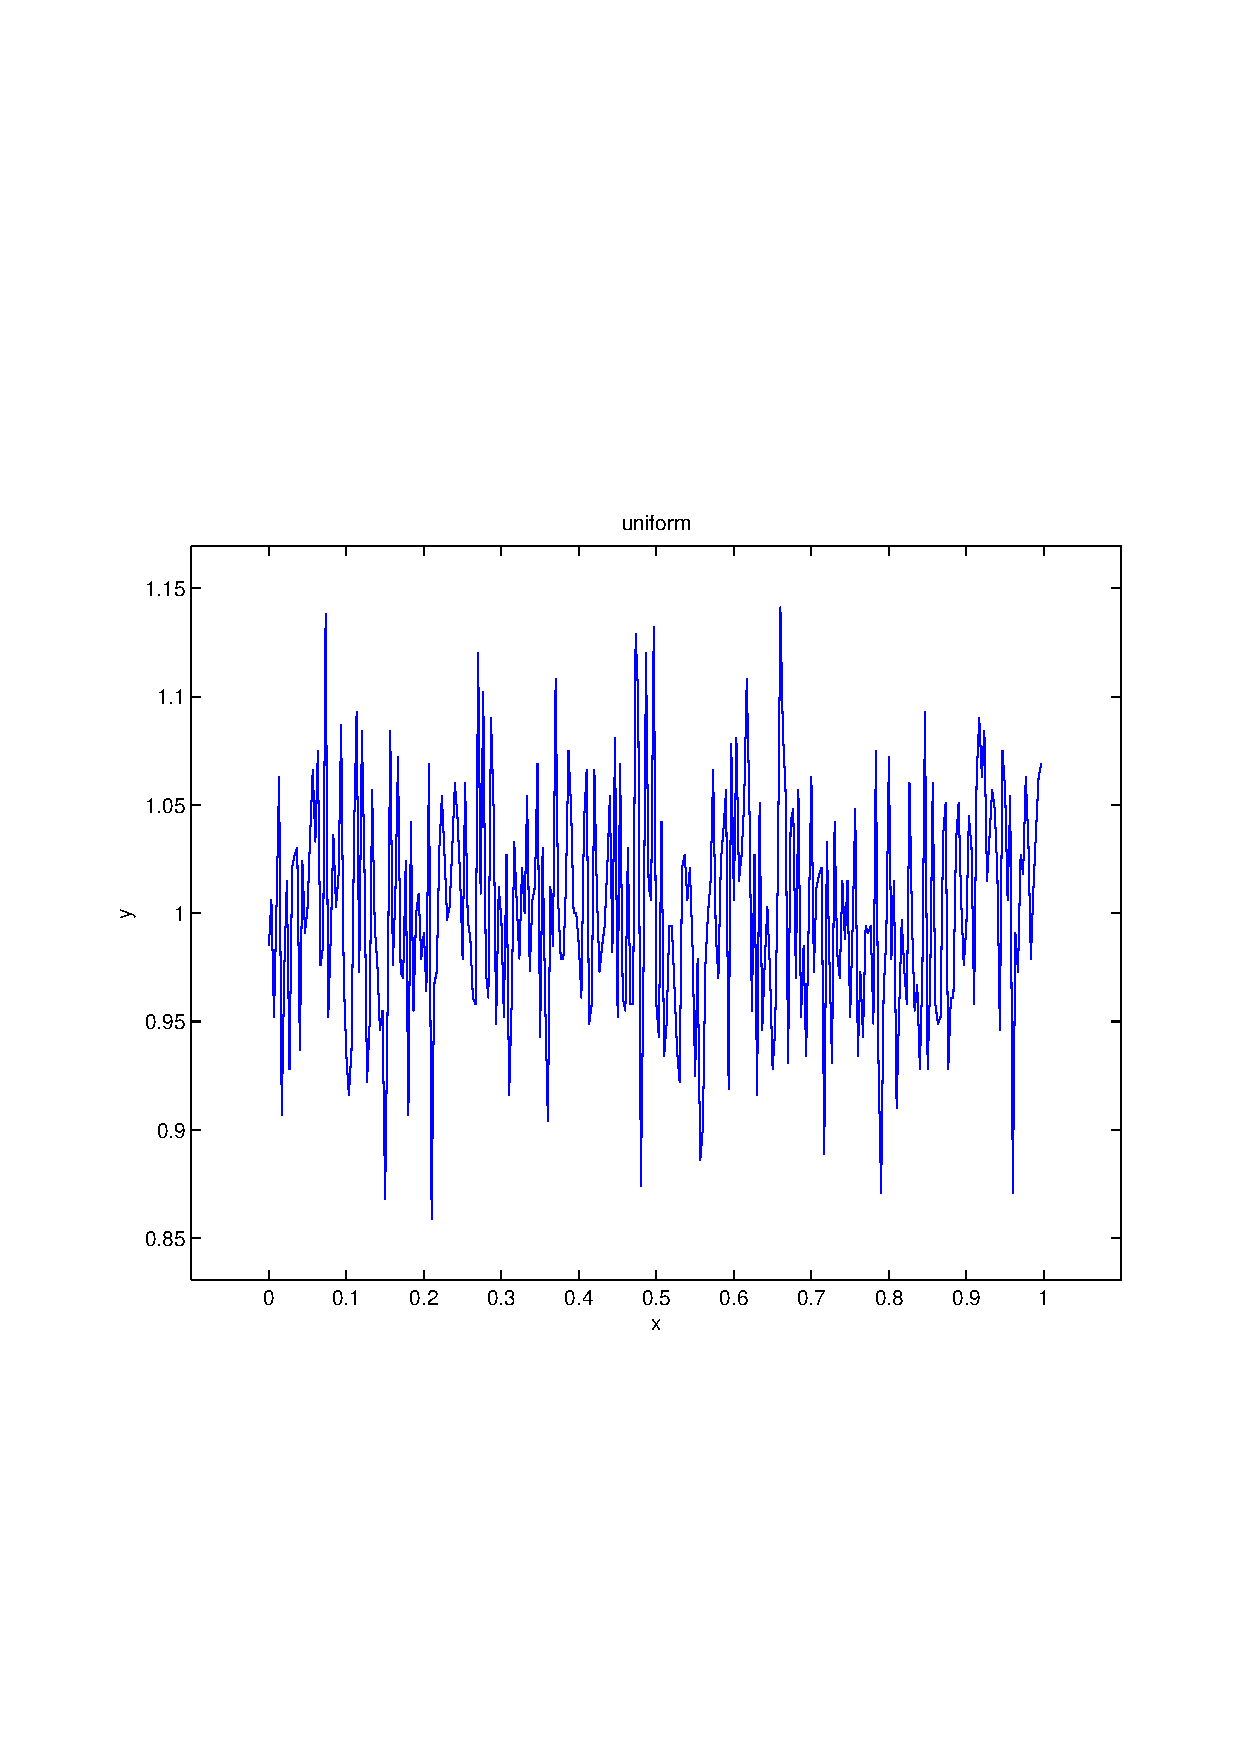
\includegraphics[width=5cm,height=5cm]{uniform.pdf}

cauchy \begin{tabular}{|c|c|c|c|}  mean & variance & skewness & kurtosis \\  \hline
$\mu_1 = +0.44288$ & $\mu_2 = +0.05341$ & $\mu_3 = +0.63935$ & $\mu_4 =+3.28094$ \\
\end{tabular}

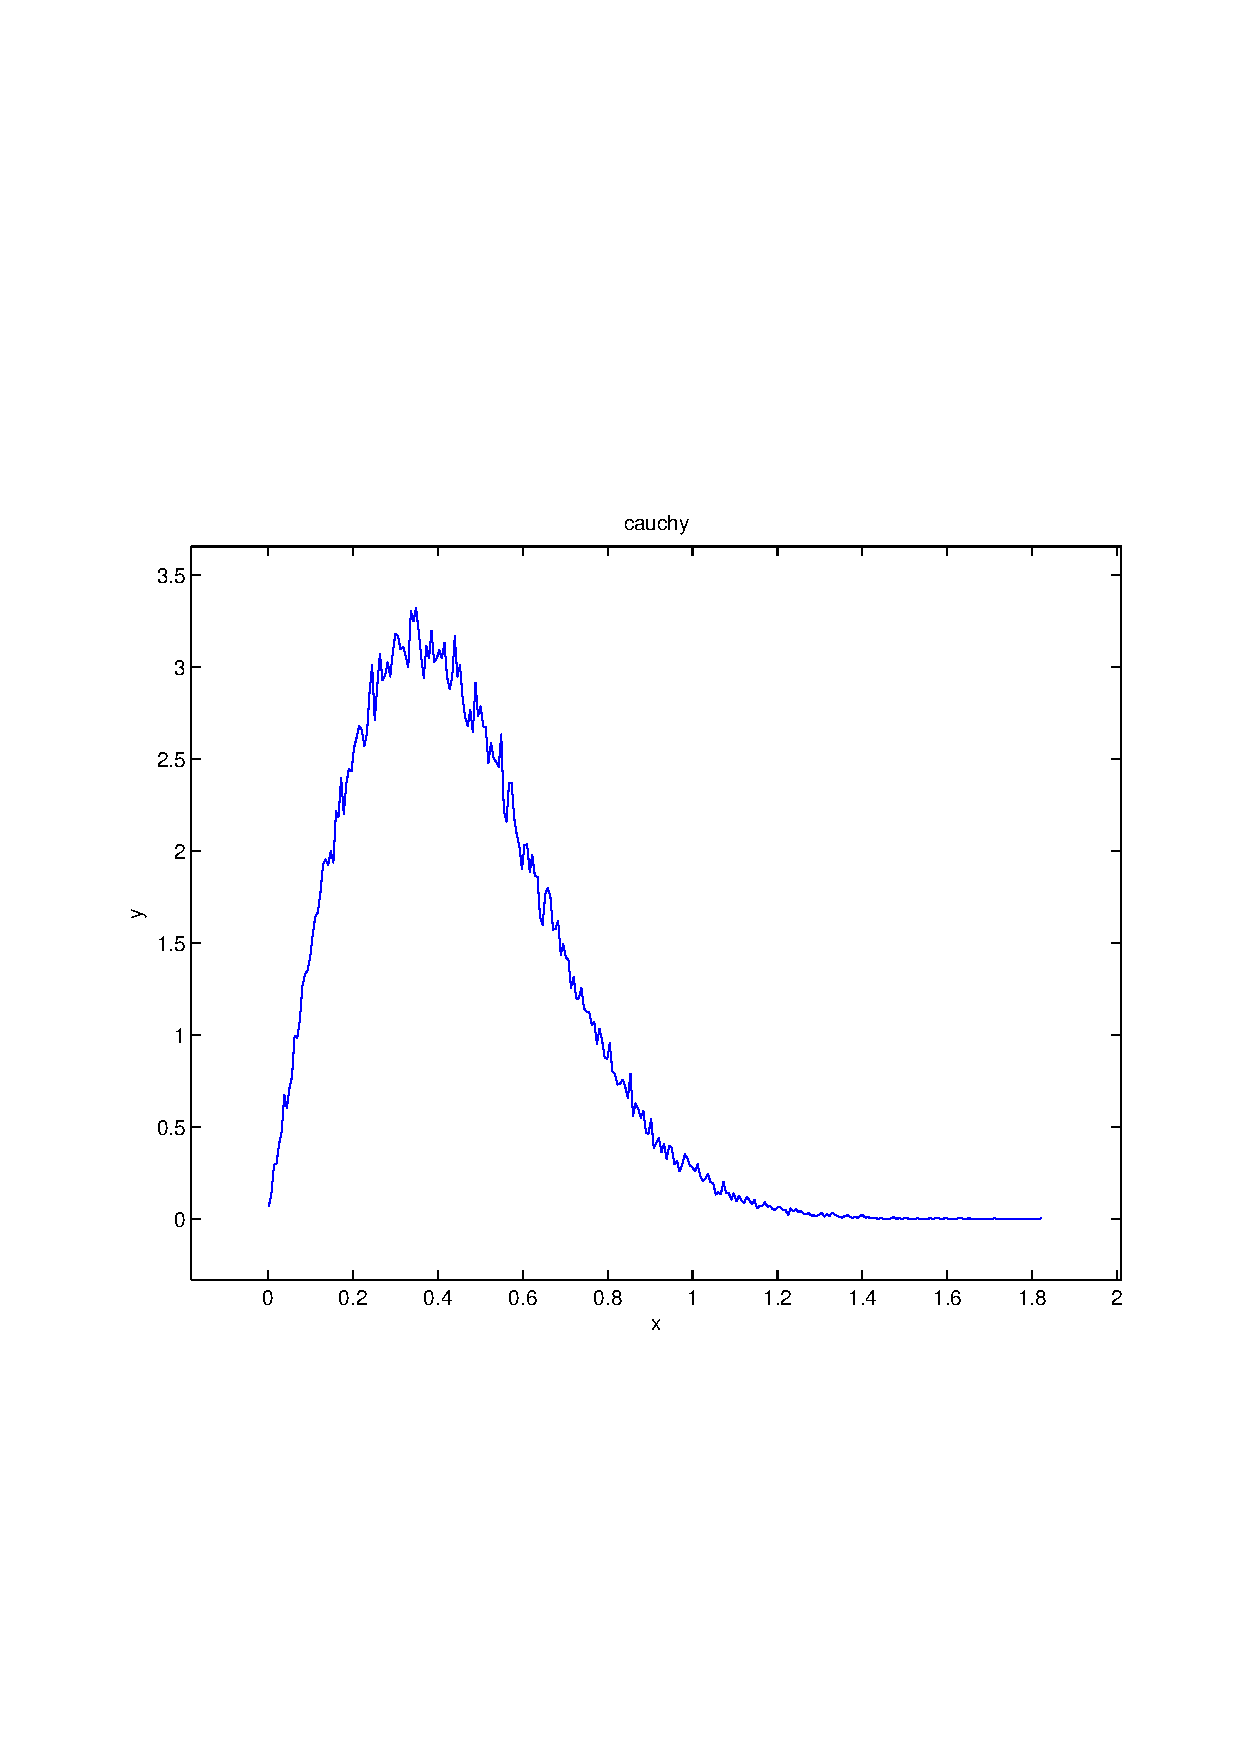
\includegraphics[width=5cm,height=5cm]{cauchy.pdf}

exponential \begin{tabular}{|c|c|c|c|}  mean & variance & skewness & kurtosis \\  \hline
$\mu_1 = +1.99647$ & $\mu_2 = +3.99339$ & $\mu_3 = +2.03097$ & $\mu_4 =+9.30842$ \\
\end{tabular}

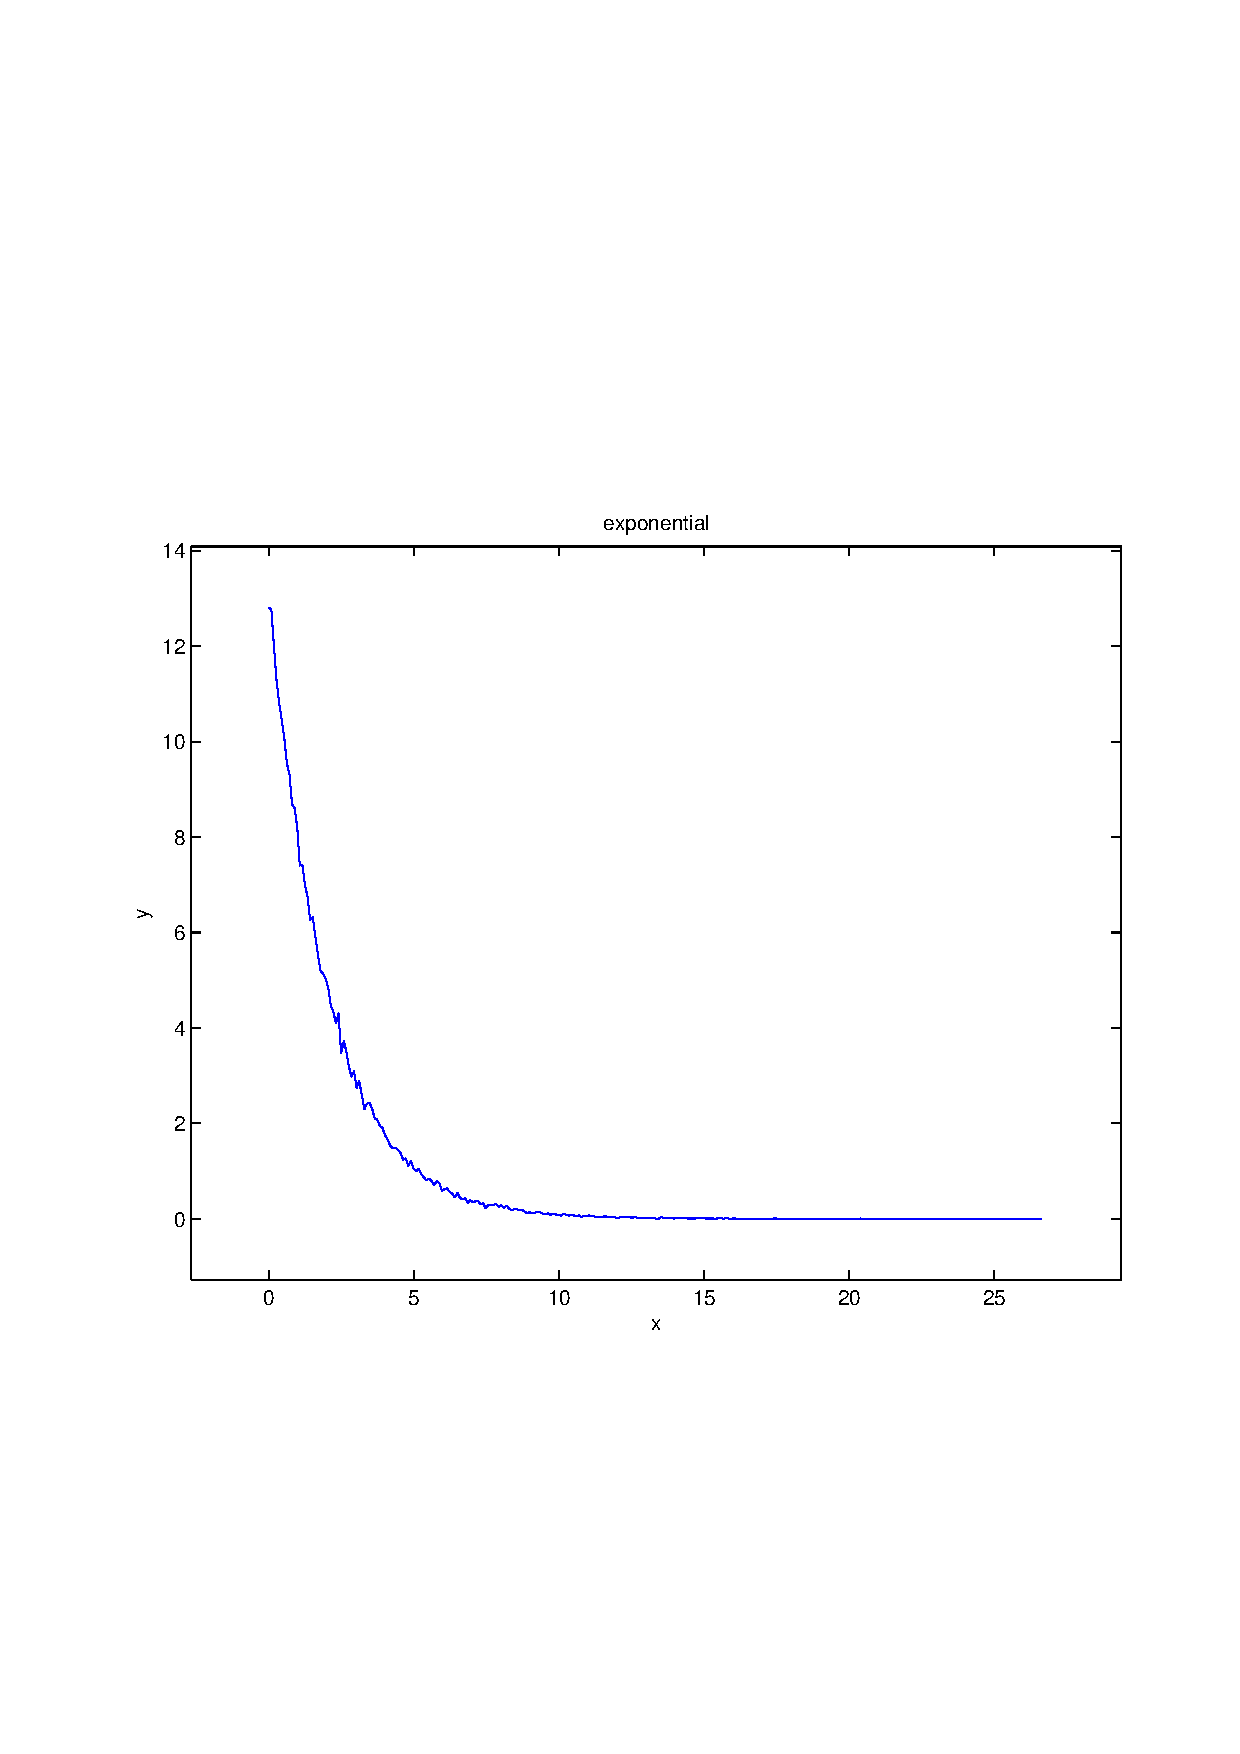
\includegraphics[width=5cm,height=5cm]{exponential.pdf}

\newpage
gamma \begin{tabular}{|c|c|c|c|}  mean & variance & skewness & kurtosis \\  \hline
$\mu_1 = +1.90412$ & $\mu_2 = +1.91731$ & $\mu_3 = +1.44468$ & $\mu_4 =+6.08156$ \\
\end{tabular}

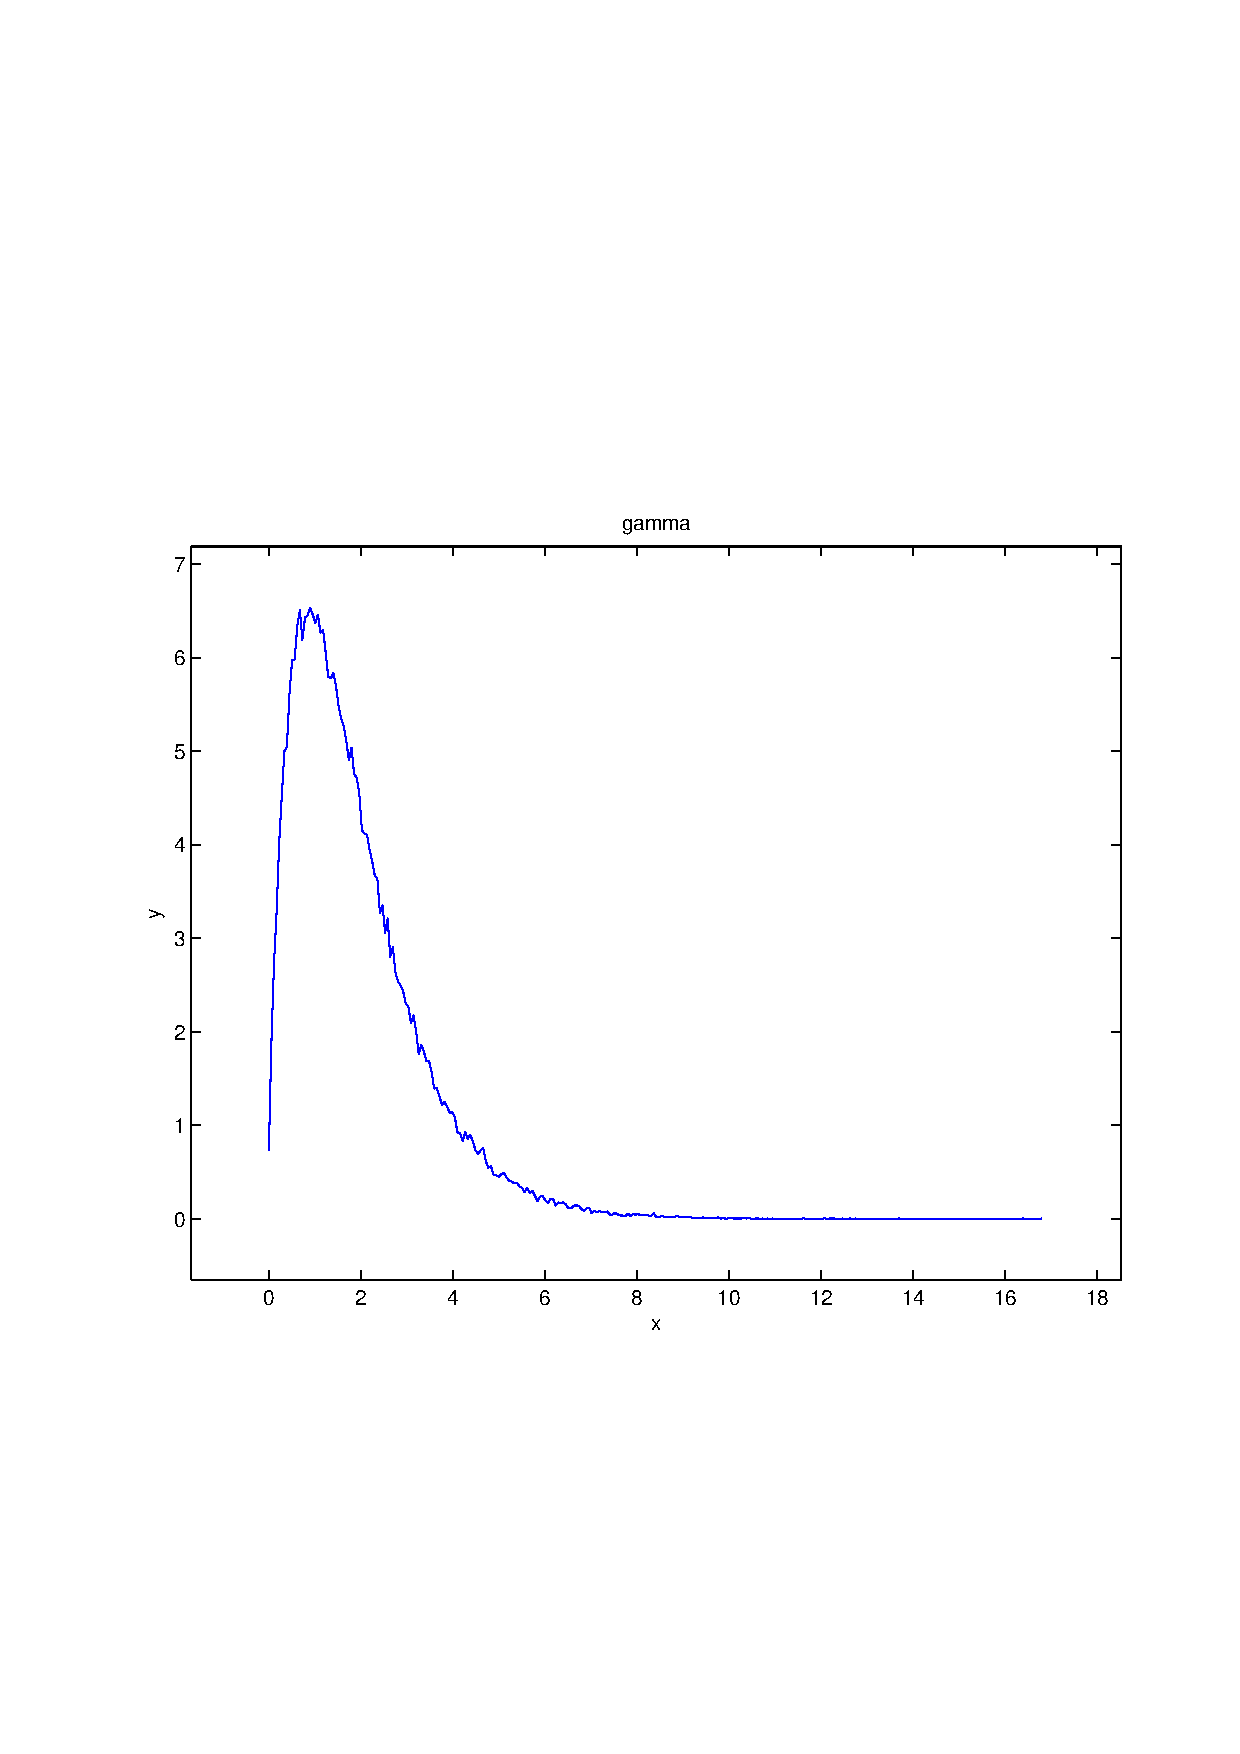
\includegraphics[width=5cm,height=5cm]{gamma.pdf}

GIG \begin{tabular}{|c|c|c|c|}  mean & variance & skewness & kurtosis \\  \hline
$\mu_1 = +0.79879$ & $\mu_2 = +10.88795$ & $\mu_3 = +15.24861$ & $\mu_4 =+314.94405$ \\
\end{tabular}

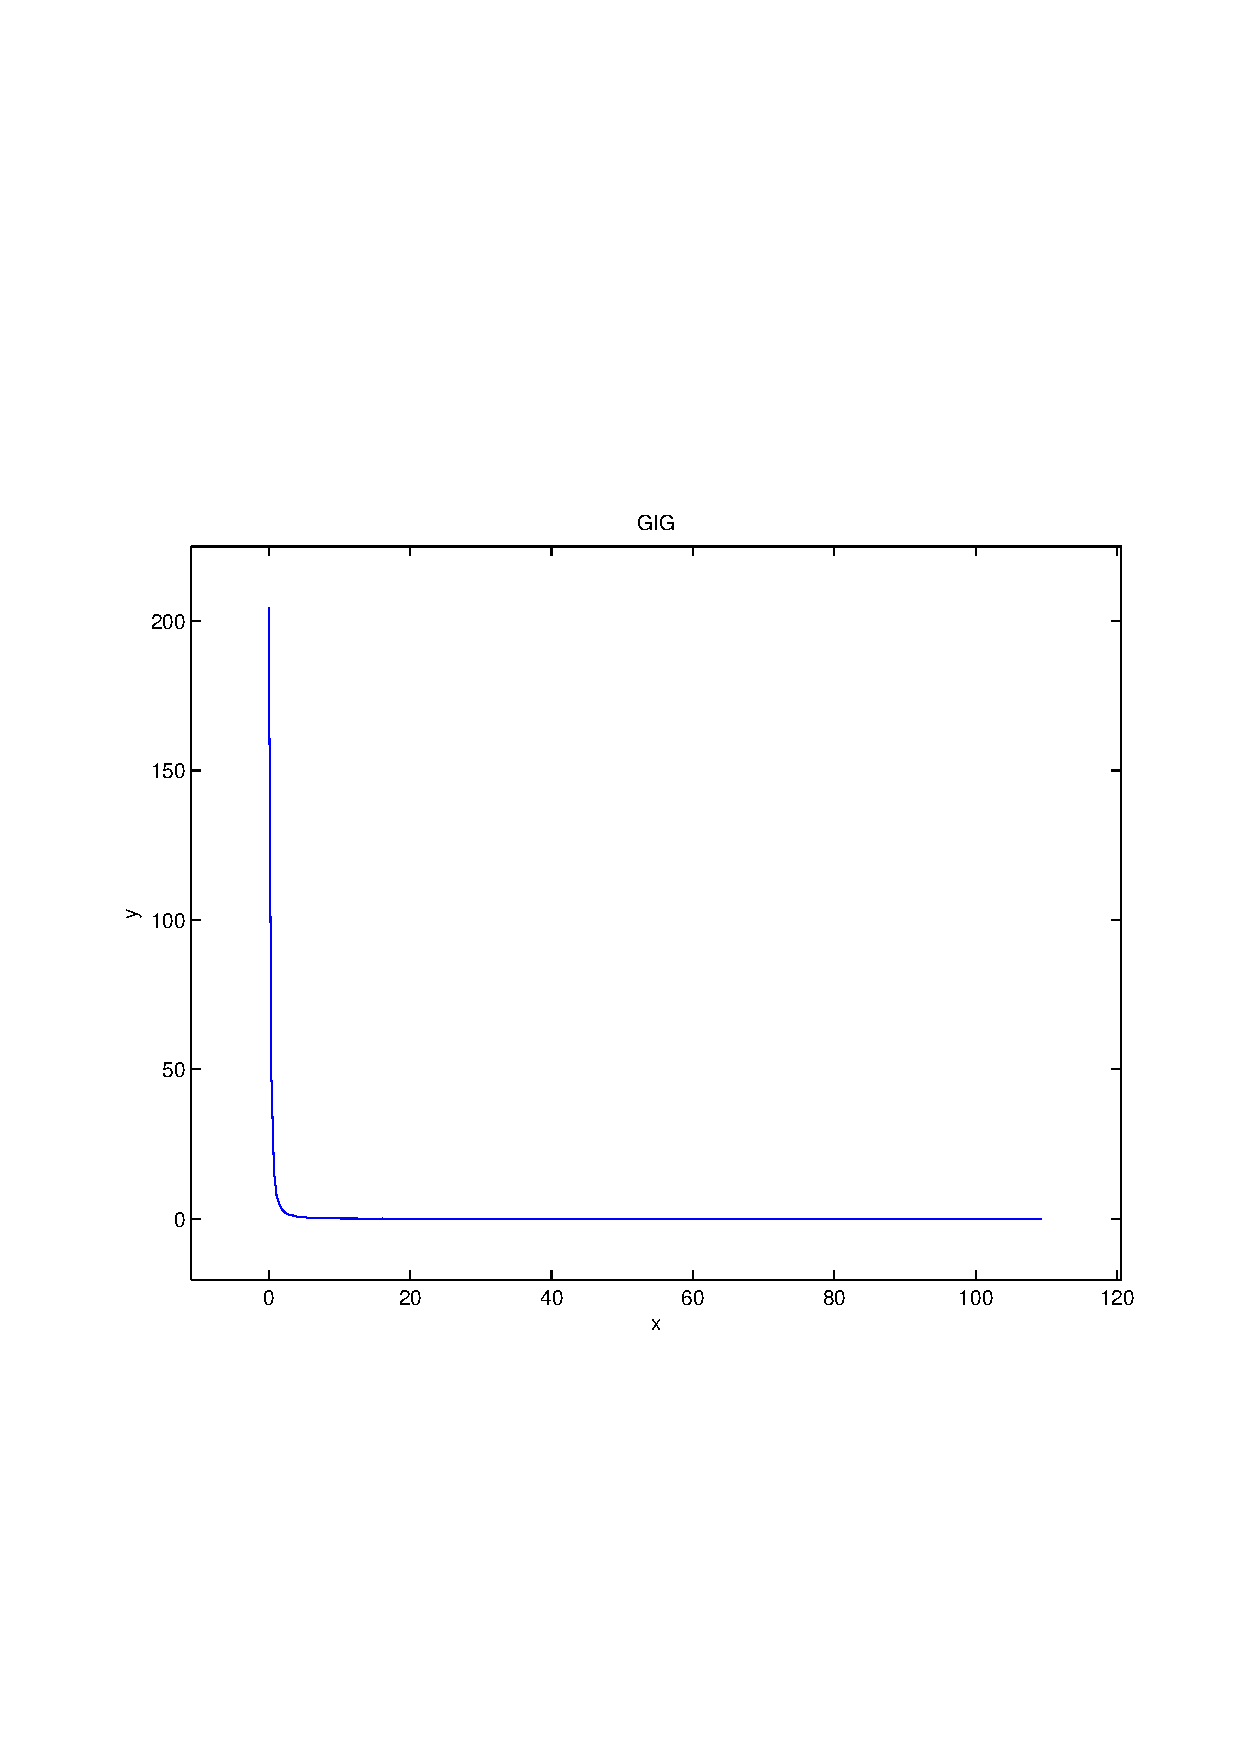
\includegraphics[width=5cm,height=5cm]{GIG.pdf}

normal-box-muller \begin{tabular}{|c|c|c|c|}  mean & variance & skewness & kurtosis \\  \hline
$\mu_1 = -0.00063$ & $\mu_2 = +0.99666$ & $\mu_3 = +0.00587$ & $\mu_4 =+3.00043$ \\
\end{tabular}

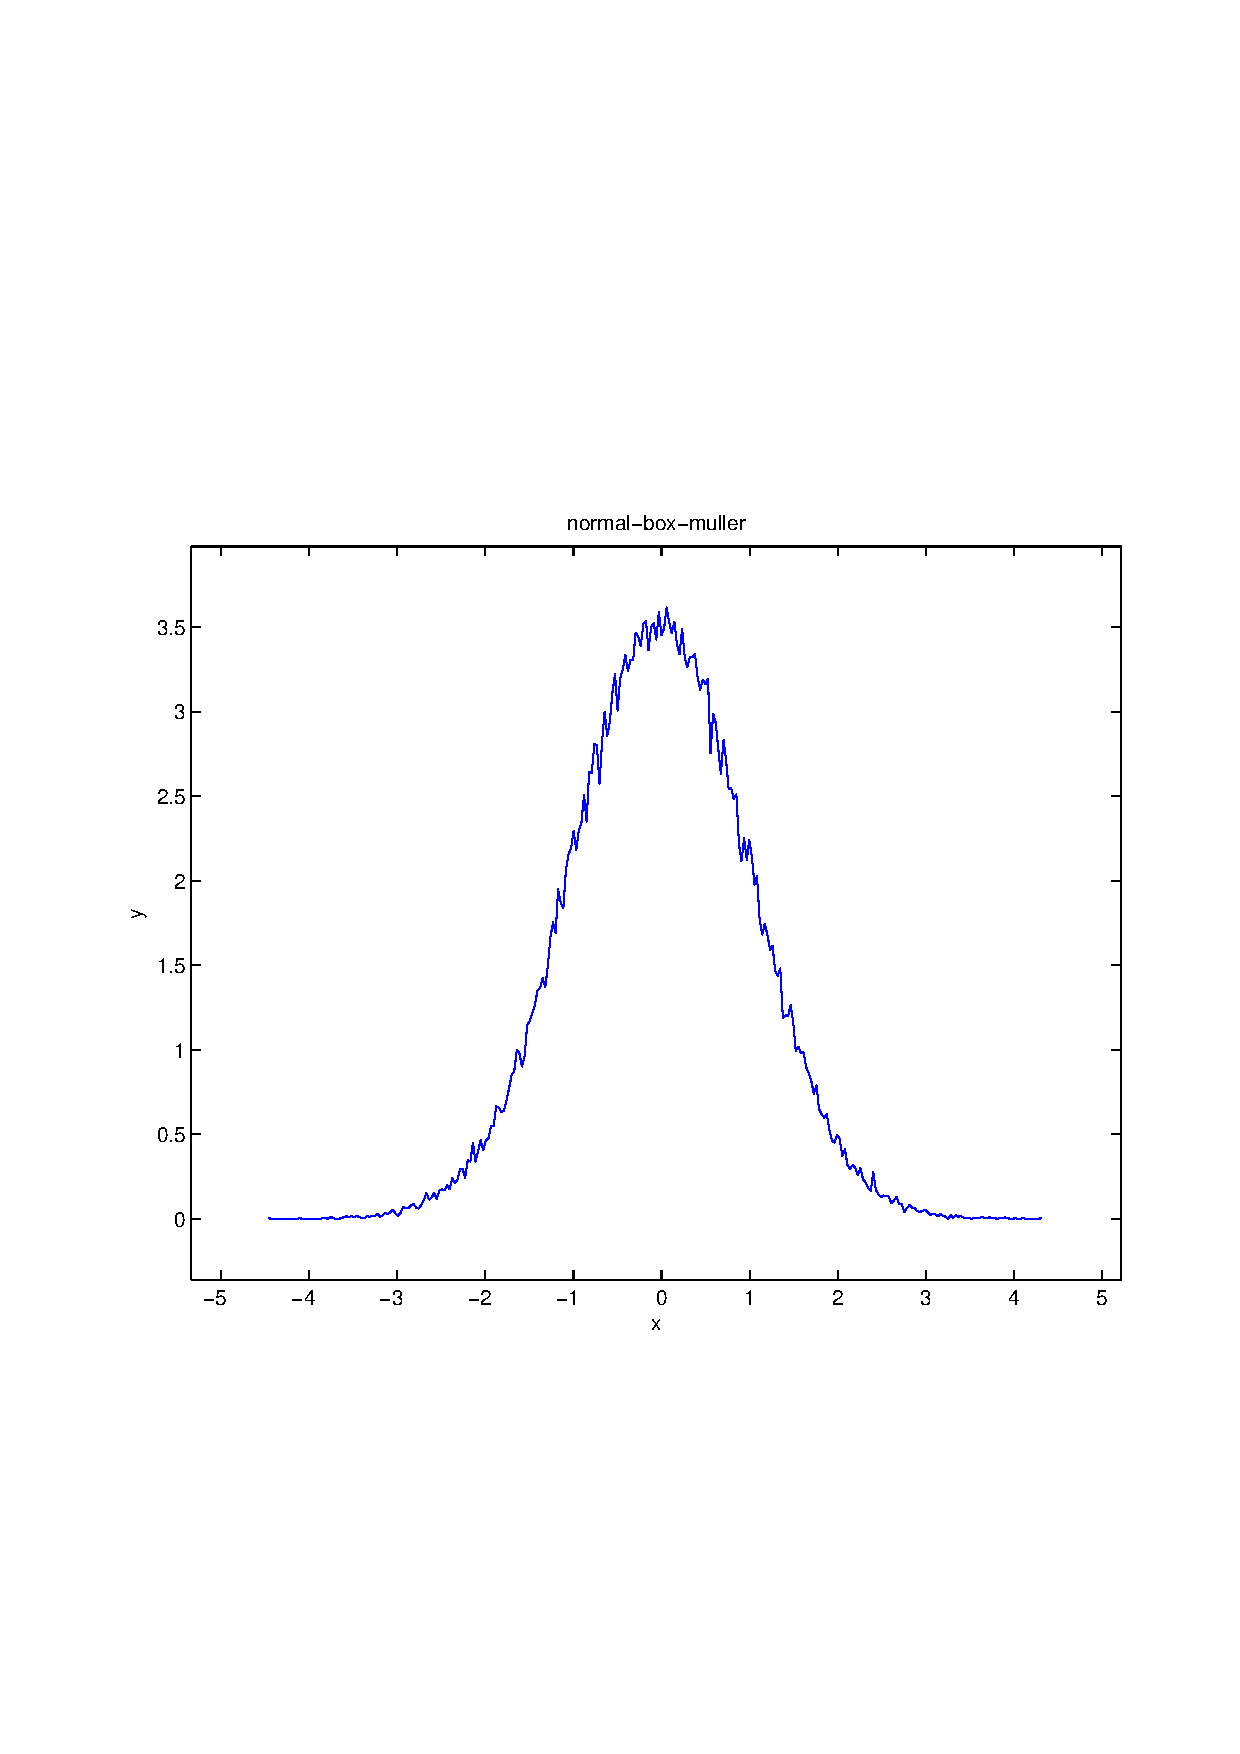
\includegraphics[width=5cm,height=5cm]{normal-box-muller.pdf}

\newpage
normal-inverse-approximation \begin{tabular}{|c|c|c|c|}  mean & variance & skewness & kurtosis \\  \hline
$\mu_1 = +0.00230$ & $\mu_2 = +1.00486$ & $\mu_3 = +0.01163$ & $\mu_4 =+2.99254$ \\
\end{tabular}

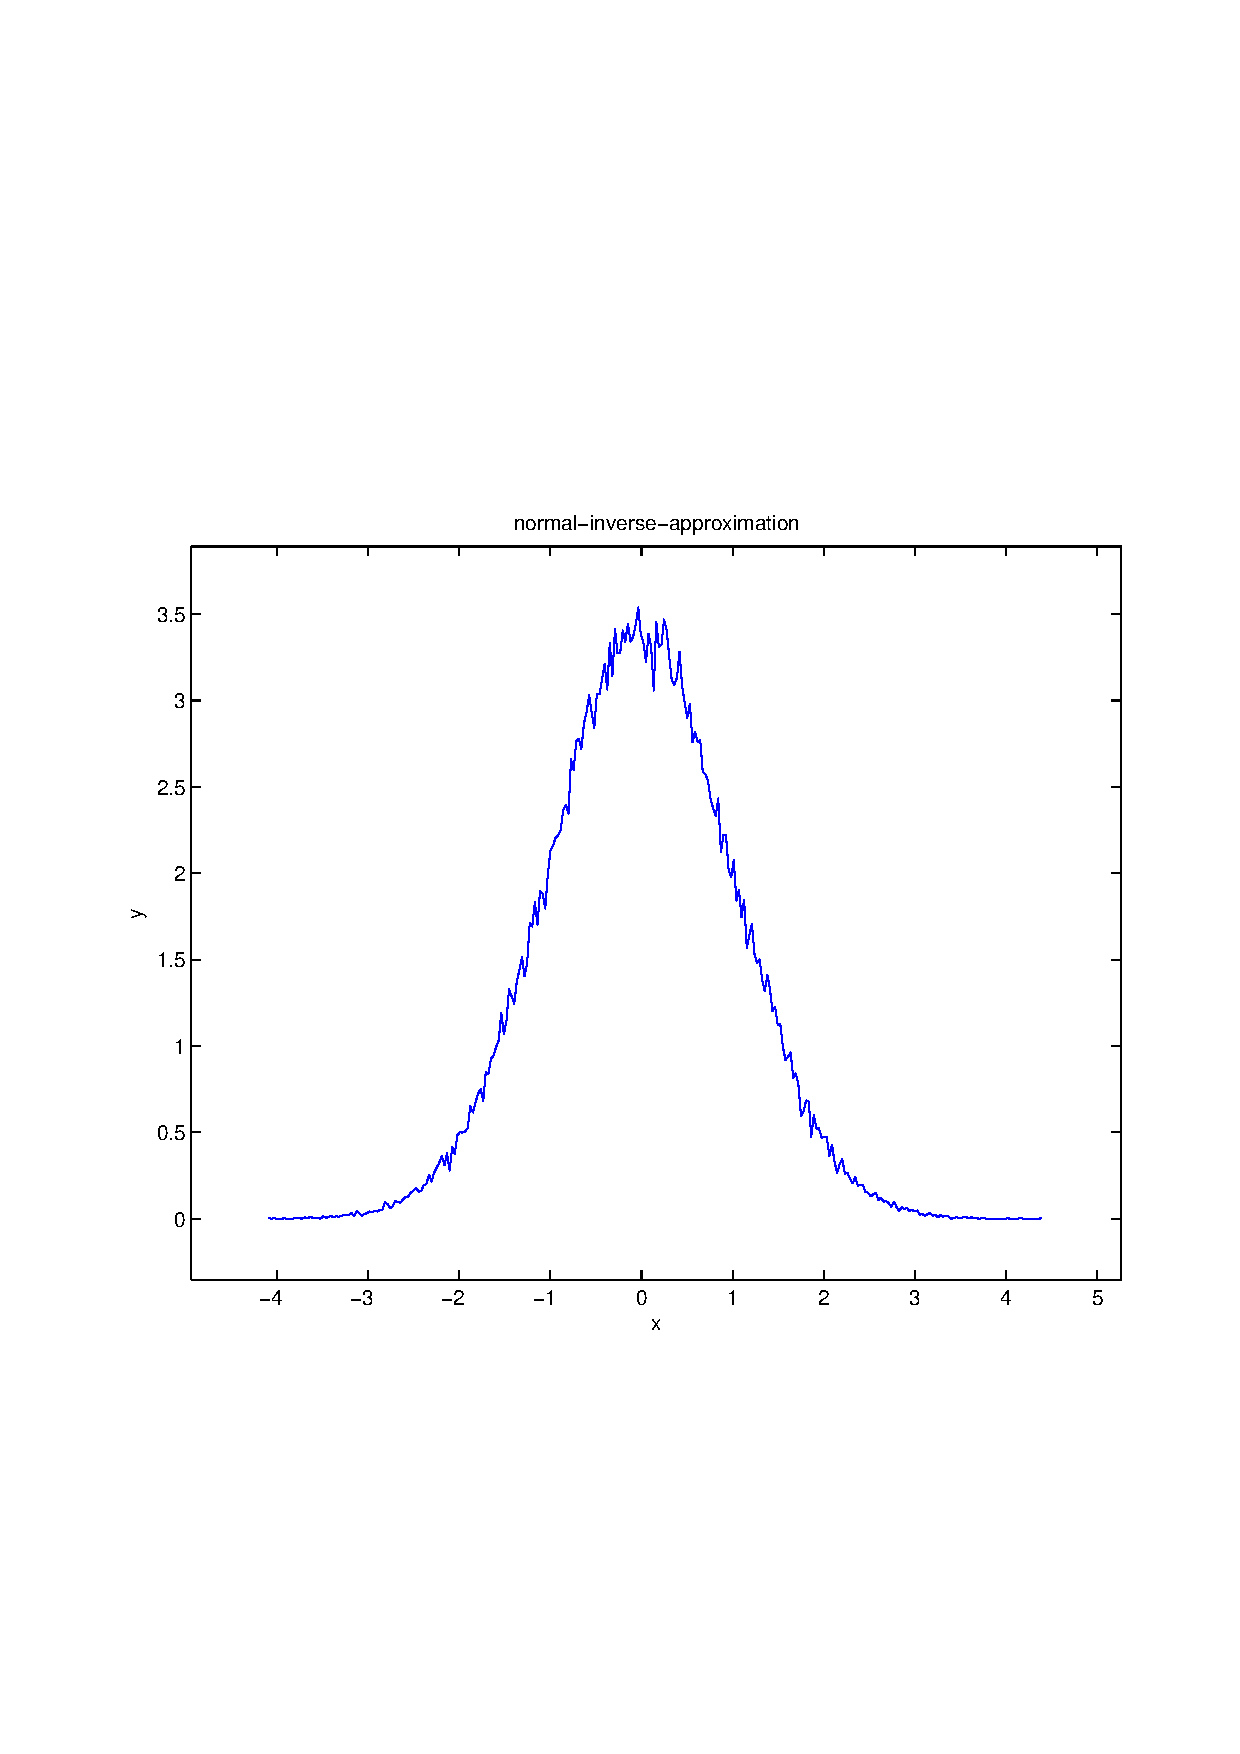
\includegraphics[width=5cm,height=5cm]{normal-inverse-approximation.pdf}

pareto \begin{tabular}{|c|c|c|c|}  mean & variance & skewness & kurtosis \\  \hline
$\mu_1 = +3184578.26493$ & $\mu_2 = +888468246174112900.00000$ & $\mu_3 = +315.36997$ & $\mu_4 =+99629.09819$ \\
\end{tabular}

\includegraphics[width=5cm,height=5cm]{pareto.pdf}

poisson \begin{tabular}{|c|c|c|c|}  mean & variance & skewness & kurtosis \\  \hline
$\mu_1 = +1.10351$ & $\mu_2 = +0.12702$ & $\mu_3 = +3.95292$ & $\mu_4 =+21.64771$ \\
\end{tabular}

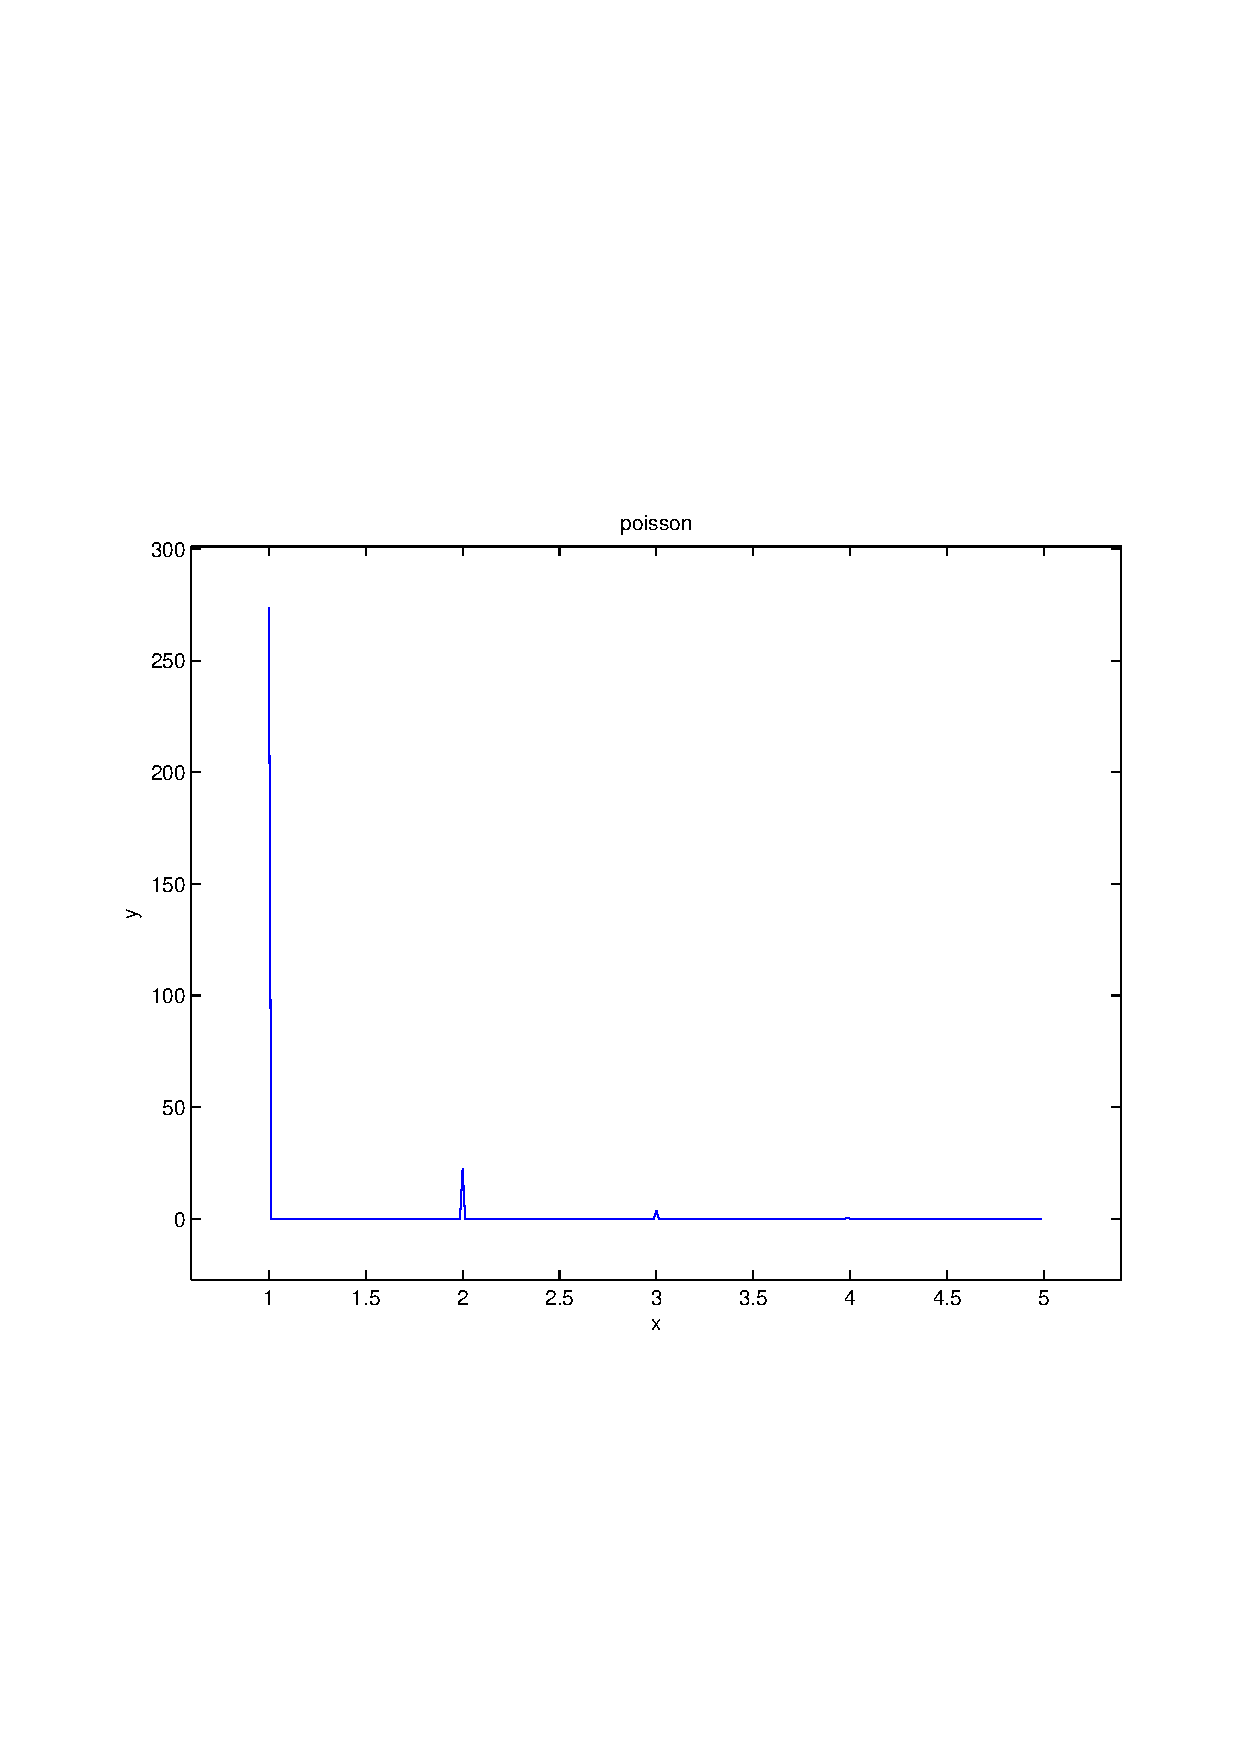
\includegraphics[width=5cm,height=5cm]{poisson.pdf}

\newpage
beta \begin{tabular}{|c|c|c|c|}  mean & variance & skewness & kurtosis \\  \hline
$\mu_1 = +0.33406$ & $\mu_2 = +0.12742$ & $\mu_3 = +0.67512$ & $\mu_4 =+1.89901$ \\
\end{tabular}

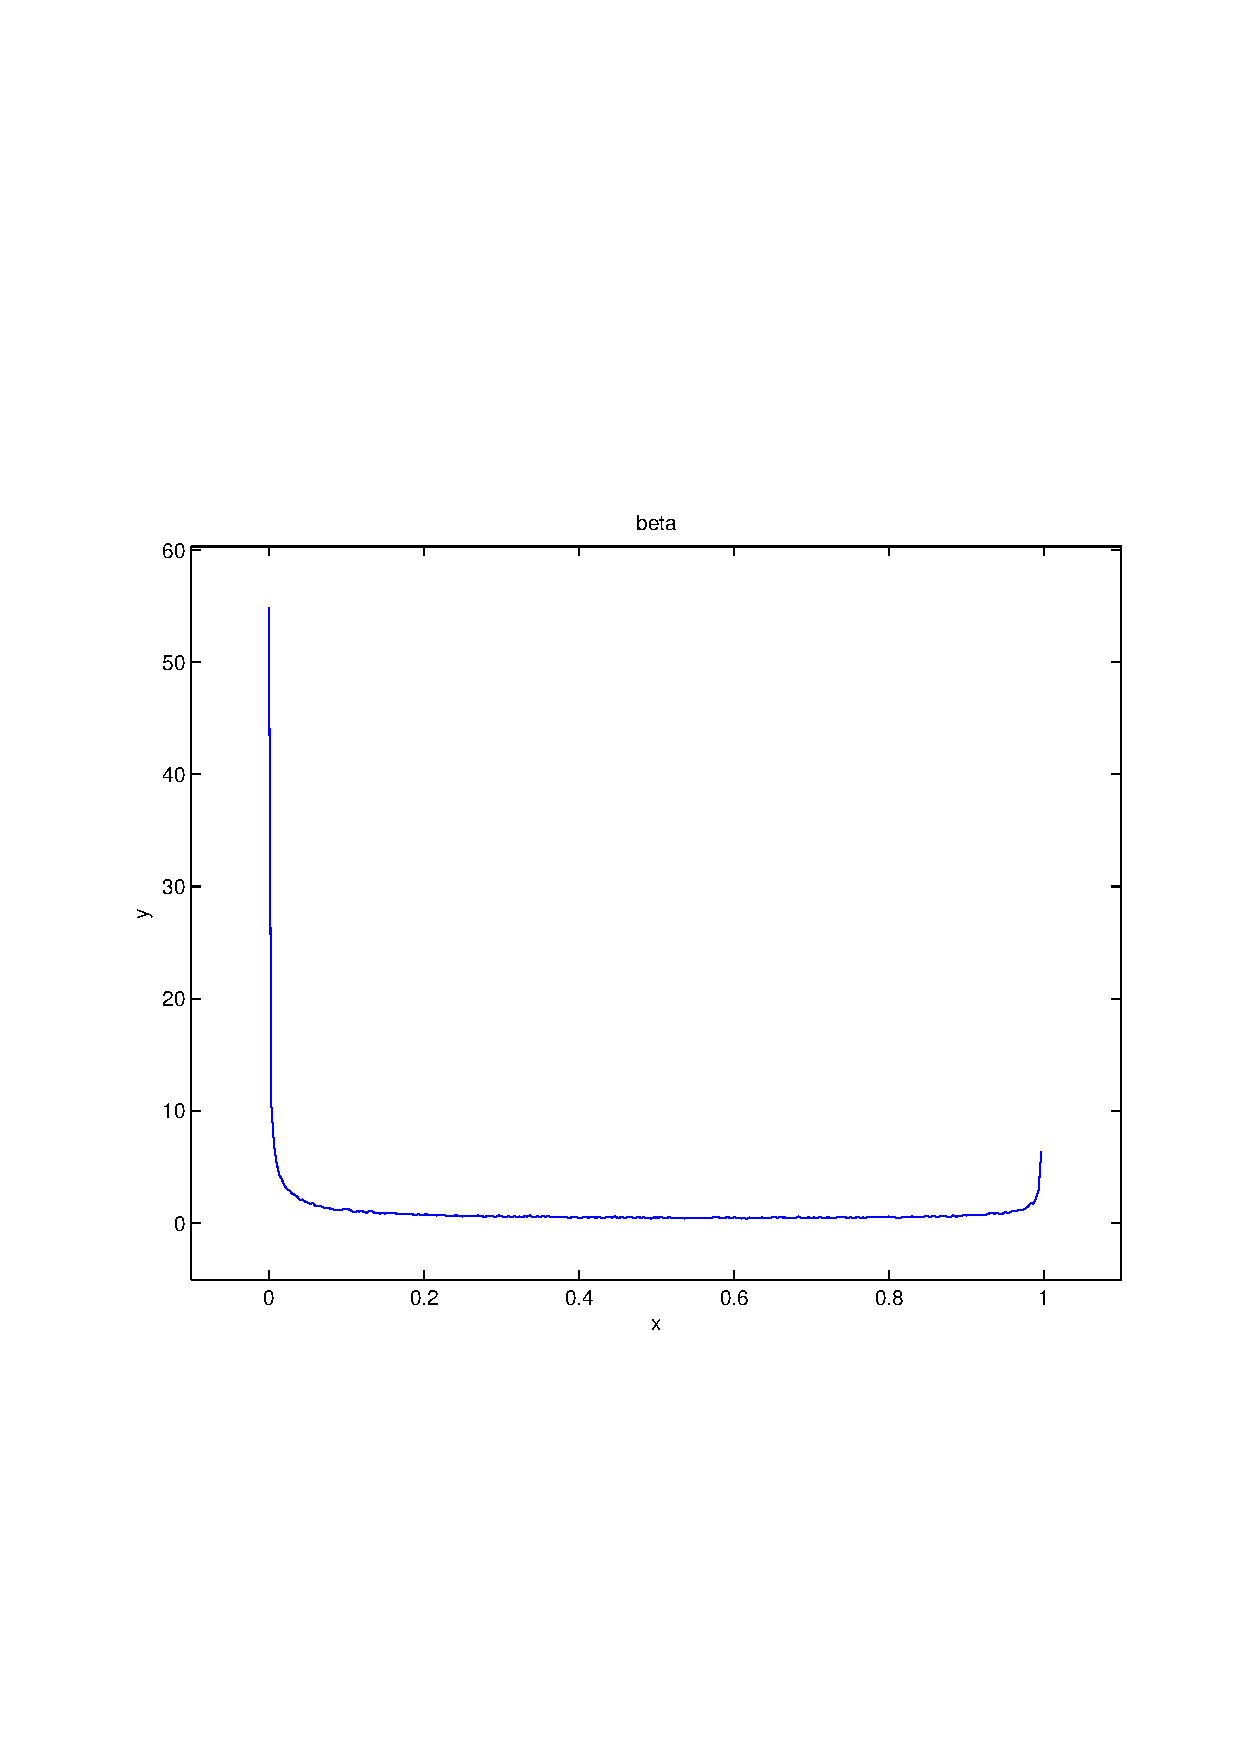
\includegraphics[width=5cm,height=5cm]{beta.pdf}

QueryPerformanceCounter  =  +10.93027
\subsubsection{Multiclass Support Vector Machine }
\begin{itemize}
\item Number or training points = 1024
\item Feature dimension = 3
\item Number or classes = 3
\end{itemize}
{The mean vectors of the 3 classes}

$\mu_1 = \left(
\begin{array}{
ccc}
+1.90000 & +0.10000 & +0.10000 \\
\end{array}
\right)$ \newline 

$\mu_2 = \left(
\begin{array}{
ccc}
+0.10000 & +1.90000 & +0.10000 \\
\end{array}
\right)$ \newline 

$\mu_3 = \left(
\begin{array}{
ccc}
+0.00000 & +0.00000 & +1.90000 \\
\end{array}
\right)$ \newline 

A random SPD covairance matrix is generated for each of the classes.\newline

$\rho_1 = \left(
\begin{array}{
ccc}
+2.989 & +0.314 & -0.450 \\
+0.314 & +4.307 & +0.301 \\
-0.450 & +0.301 & +3.316 \\
\end{array}
\right)$ \newline 

$\rho_2 = \left(
\begin{array}{
ccc}
+3.318 & +0.437 & -0.124 \\
+0.437 & +3.356 & -0.271 \\
-0.124 & -0.271 & +3.303 \\
\end{array}
\right)$ \newline 

$\rho_3 = \left(
\begin{array}{
ccc}
+3.367 & -0.294 & +0.226 \\
-0.294 & +3.712 & +0.486 \\
+0.226 & +0.486 & +3.866 \\
\end{array}
\right)$ \newline 

Verify $L_1$ condition number of covariance. The diagonal entries of the matrix have the form $(0.5 + U(0,1) )*dim(Dom(Cov))$
The lower-diagonal entries take the form $U(0,1) - 0.5$. 
The $L_1$ condition numbers are :
\begin{itemize}
\item +2.083
\item +1.369
\item +1.594
\end{itemize}
\includegraphics[width=10.0cm,height=10.0cm]{rv1_corr.pdf}

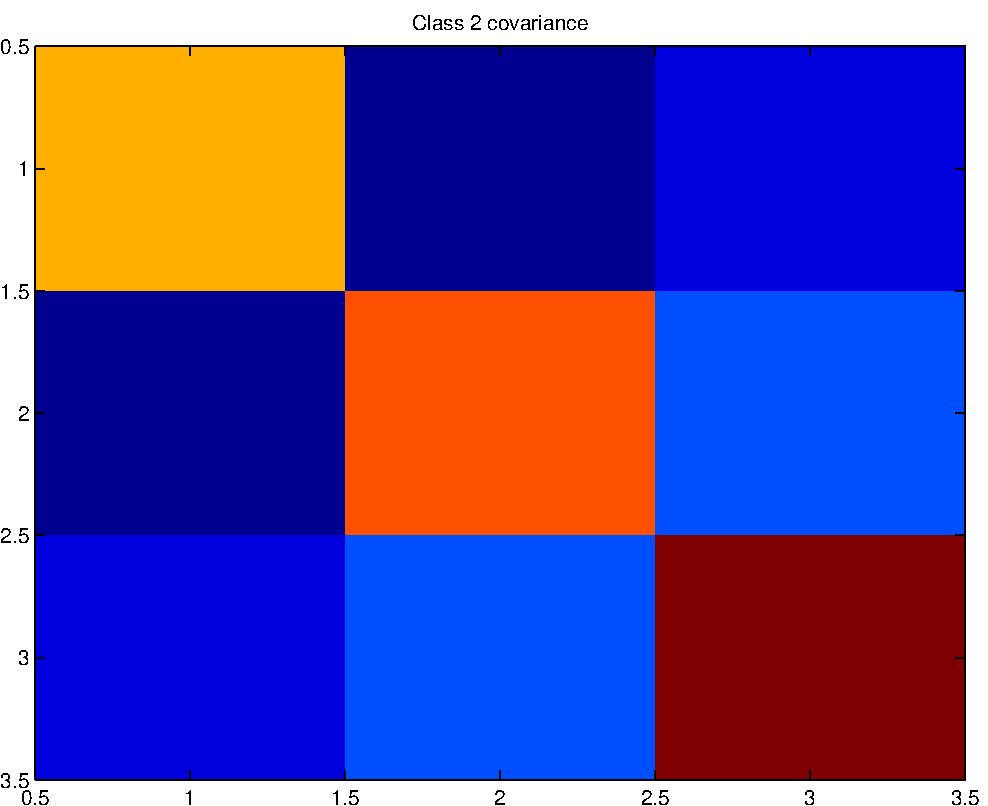
\includegraphics[width=10.0cm,height=10.0cm]{rv2_corr.pdf}

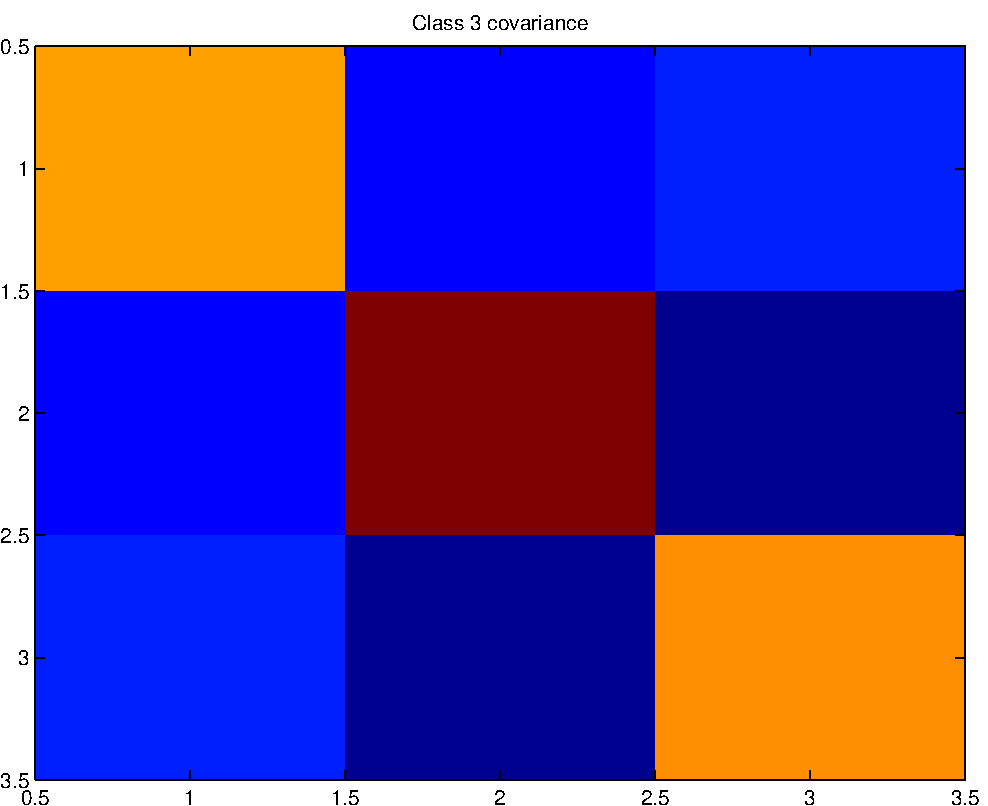
\includegraphics[width=10.0cm,height=10.0cm]{rv3_corr.pdf}

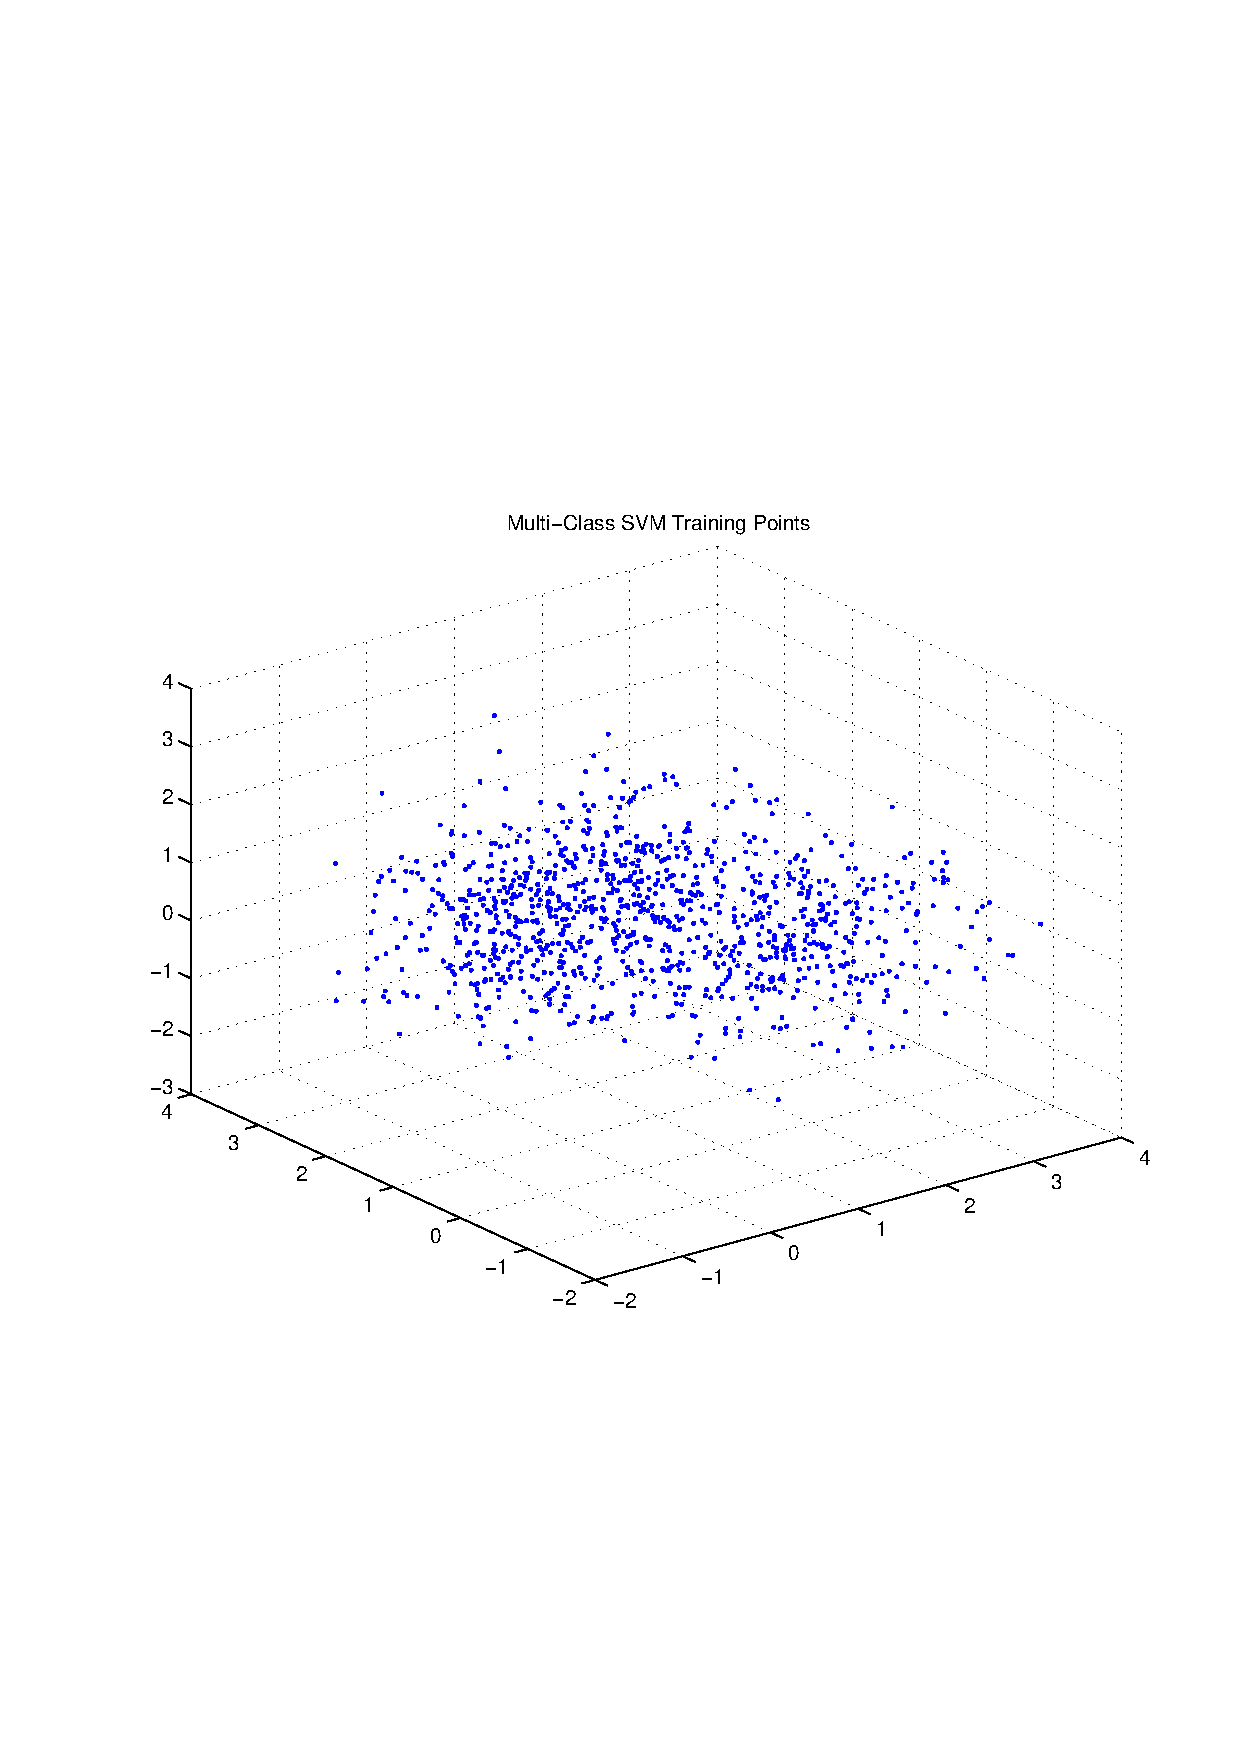
\includegraphics[width=10.0cm,height=10.0cm]{trainingPoints.pdf}

These are the SVM parameters - the RBF kernel is used\begin{itemize}
\item allOutlierFraction=0.05
\item mixingCoeff=0.3
\item smoThresh=1.0/10000.0
\item sigma=1
\end{itemize}
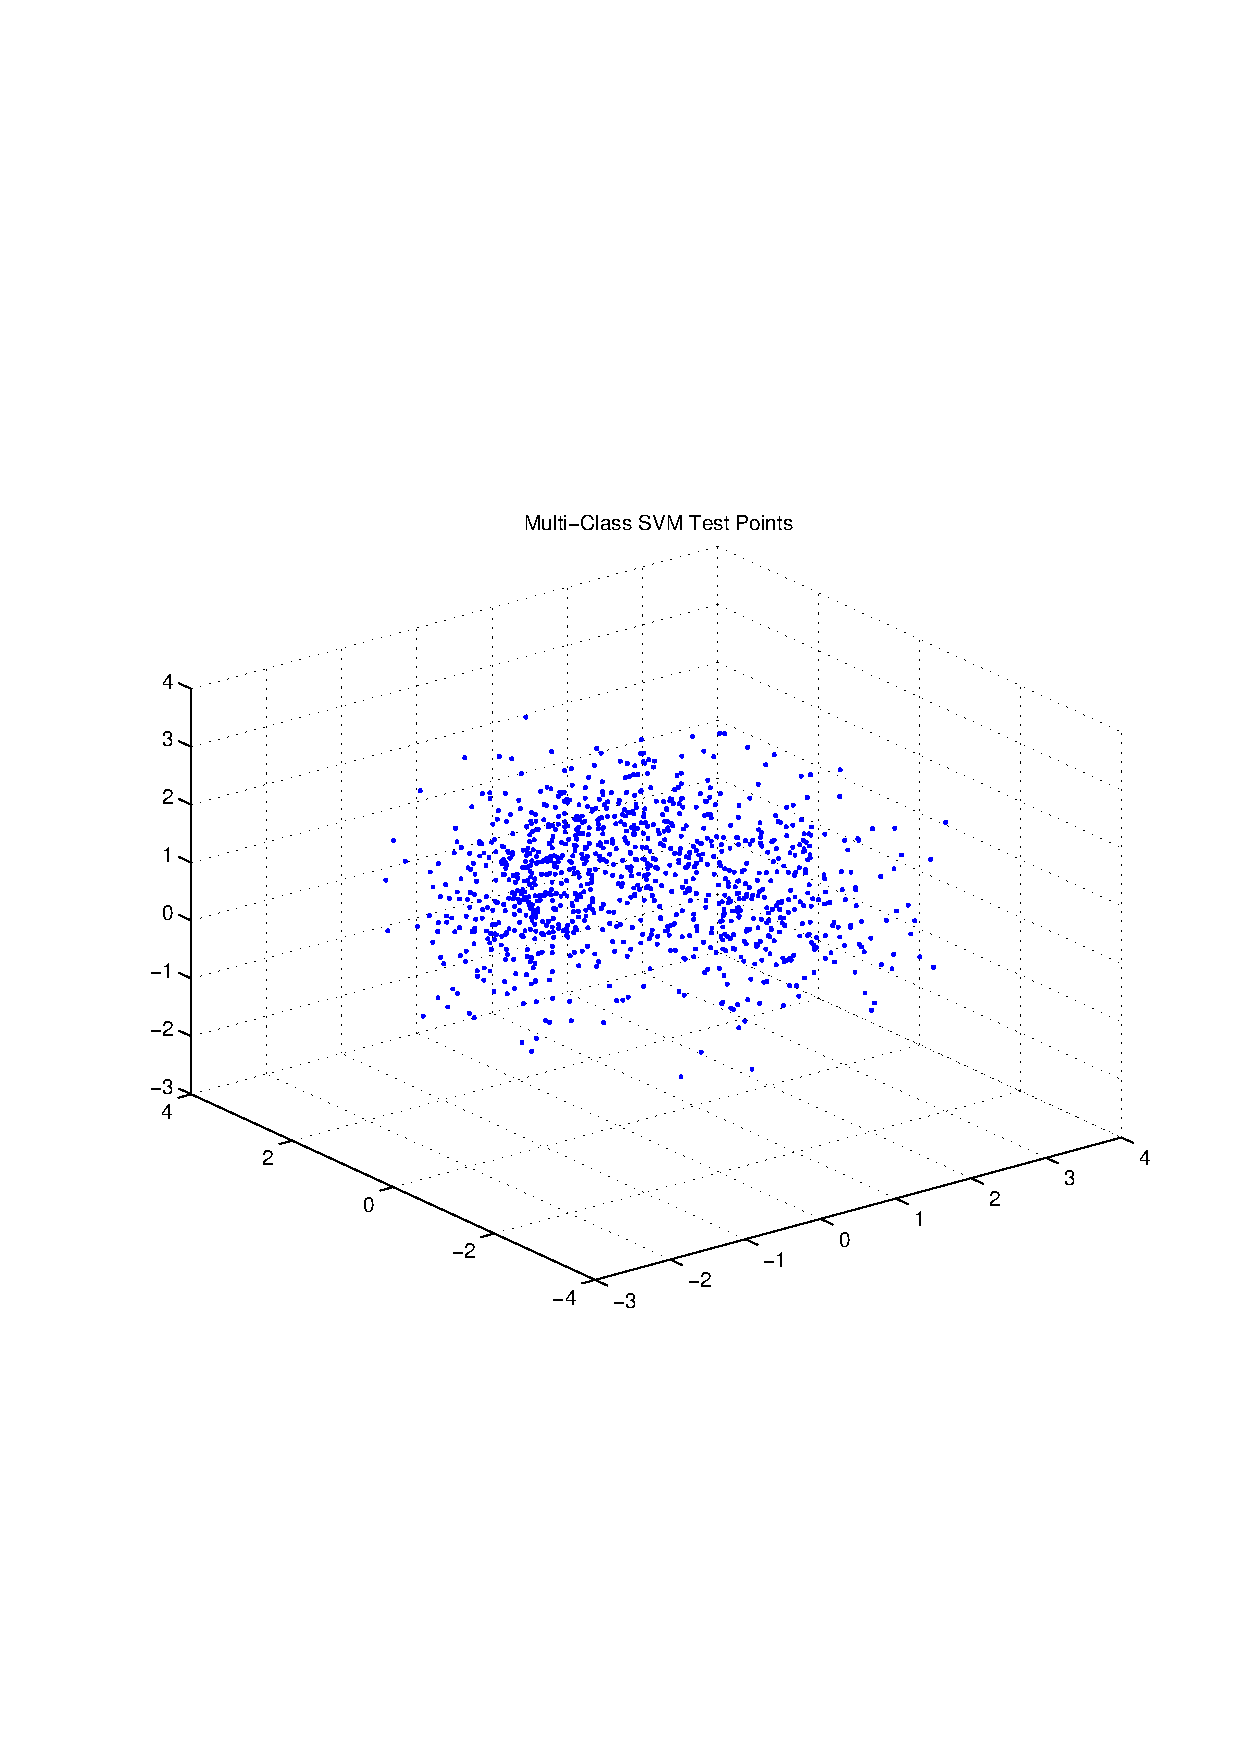
\includegraphics[width=10.0cm,height=10.0cm]{testPoints.pdf}

The marginal sample moments (mean var skew kurtosis) for training points.\newline
\begin{tabular}{ c |  c  c  c  c}
Feature & $\mu_1$ & $\mu_2$ & $\mu_3$ & $\mu_4$ \\
0 & +0.669 & +1.407 & +0.162& +2.343 \\
\hline
1 & +0.709 & +1.414 & +0.225& +2.405 \\
\hline
2 & +0.704 & +1.402 & +0.367& +2.597 \\
\hline
\end{tabular}
\newline
The marginal sample moments (mean var skew kurtosis) for test points.\newline
\begin{tabular}{ c | c  c  c  c}
Feature & $\mu_1$ & $\mu_2$ & $\mu_3$ & $\mu_4$ \\
0 & +0.677 & +1.300 & +0.310& +2.431\\
\hline
1 & +0.669 & +1.413 & +0.253& +2.404\\
\hline
2 & +0.723 & +1.326 & +0.325& +2.449\\
\hline
\end{tabular}\newline
\includegraphics[width=10.0cm,height=10.0cm]{classDiffs.pdf}

The error rate for this run is +0.313\newline
QueryPerformanceCounter  =  +6.483
\subsubsection{Semidefinite Programming SDPA}
QueryPerformanceCounter  =  +0.024
\subsubsection{Linear Regression 3x1}
\subsubsection{3 x 1 Linear Regression}
Sample size = 64

Number of features = 3

$\sigma = \left(
\begin{array}{
ccc}
+3.952 & -0.499 & -0.010 \\
-0.499 & +1.895 & +0.465 \\
-0.010 & +0.465 & +4.477 \\
\end{array}
\right)$ \newline 

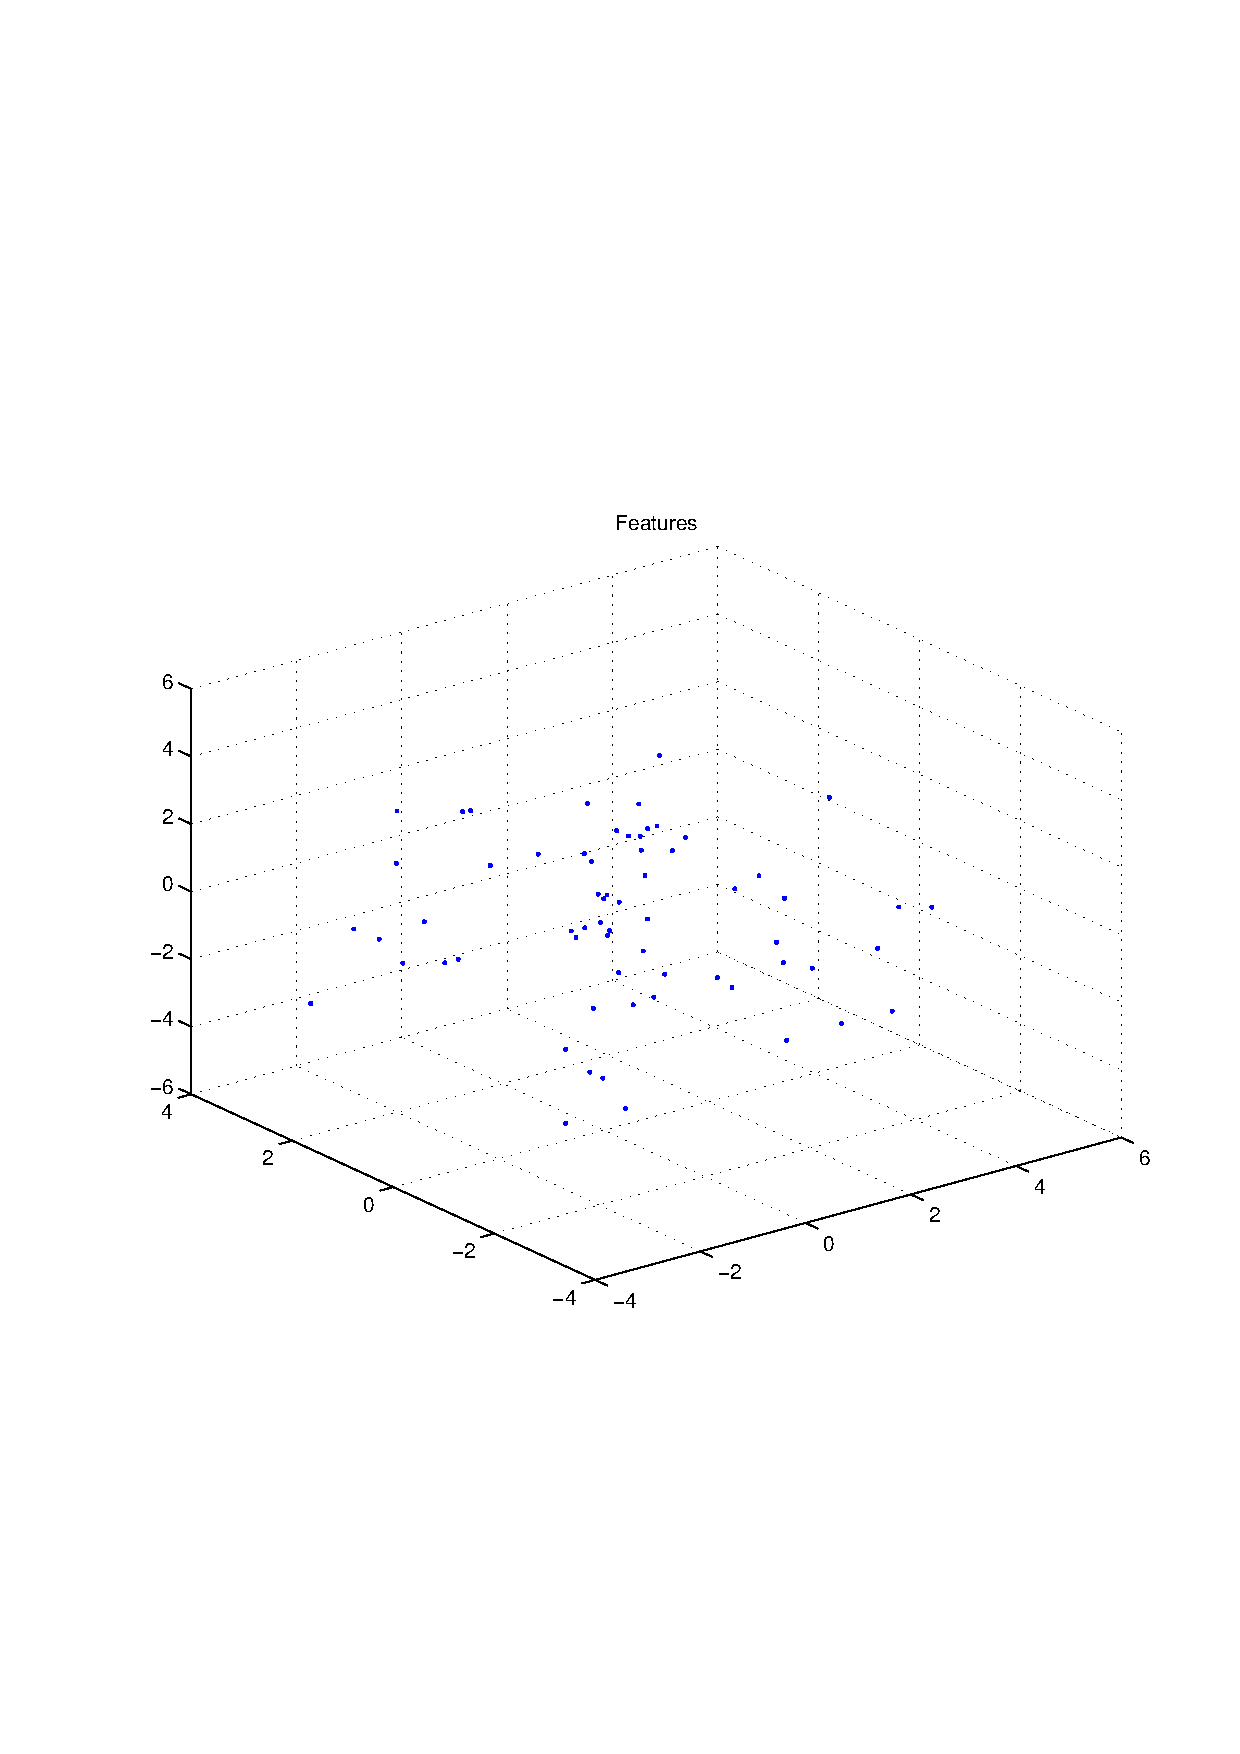
\includegraphics[width=10.0cm,height=10.0cm]{regression_features.pdf}

Beta
+0.817, +0.999, +0.510

Response
+0.912
+1.969
+2.740
+1.442
-3.382
+3.297
-2.445
+1.314
-1.261
+2.126
+3.806
+0.638
+1.434
+2.235
+1.266
+3.648
+0.257
+2.625
-1.018
+2.481
+0.180
+2.575
+1.437
+0.256
+2.231
+2.942
-0.421
-0.721
-1.354
+1.362
+1.050
-1.175
+3.344
+3.751
-0.217
+1.149
+0.953
-0.314
+1.834
+3.515
-0.847
+1.654
-3.066
-7.105
+0.771
+0.377
+2.042
+1.775
+0.844
+2.520
-0.411
-0.268
-3.698
-3.851
-1.757
-2.007
+0.400
+1.902
+0.645
+1.422
+1.952
+4.213
-2.547
+0.322
Estimate for Beta
+16.805
+16.055
+8.990
Error:
+0.000, -0.000, +0.000


QueryPerformanceCounter  =  +1.047
\subsubsection{Matrix Norms}
\subsubsection{Haar Distributed Random Orthogonal Matrix $A \in O(n)$}
 Testing Operator Norm
Number of Dimensions: 12

$A = \left(
\begin{array}{
cccccccccccc}
-0.066 & -0.282 & +0.081 & +0.202 & +0.270 & +0.529 & +0.195 & +0.233 & +0.498 & +0.118 & -0.391 & +0.092 \\
-0.056 & +0.147 & +0.348 & -0.312 & +0.321 & +0.290 & -0.192 & +0.258 & -0.275 & +0.378 & +0.139 & -0.477 \\
-0.252 & +0.253 & +0.132 & +0.335 & -0.576 & +0.104 & +0.209 & -0.168 & -0.159 & +0.362 & -0.340 & -0.236 \\
-0.033 & +0.033 & -0.033 & +0.418 & -0.118 & +0.305 & +0.240 & +0.470 & -0.302 & -0.433 & +0.389 & -0.076 \\
+0.043 & -0.031 & +0.389 & -0.077 & +0.245 & -0.147 & +0.713 & -0.144 & -0.239 & +0.181 & +0.130 & +0.349 \\
-0.341 & +0.126 & +0.447 & -0.339 & -0.418 & +0.078 & -0.165 & +0.237 & +0.280 & -0.090 & +0.188 & +0.409 \\
+0.569 & +0.658 & +0.057 & -0.070 & +0.018 & +0.347 & -0.021 & -0.115 & +0.011 & -0.167 & -0.182 & +0.201 \\
+0.147 & -0.386 & +0.085 & +0.152 & -0.133 & +0.478 & -0.288 & -0.489 & -0.183 & +0.178 & +0.341 & +0.223 \\
+0.183 & +0.222 & -0.189 & +0.137 & -0.074 & -0.069 & +0.176 & +0.024 & +0.542 & +0.413 & +0.579 & -0.148 \\
-0.088 & -0.117 & -0.211 & -0.555 & -0.196 & +0.319 & +0.407 & -0.293 & +0.109 & -0.299 & +0.056 & -0.360 \\
+0.641 & -0.412 & +0.149 & -0.163 & -0.419 & -0.135 & +0.063 & +0.357 & -0.041 & +0.120 & -0.134 & -0.104 \\
-0.108 & +0.049 & -0.625 & -0.269 & -0.075 & +0.178 & +0.060 & +0.294 & -0.289 & +0.387 & -0.048 & +0.401 \\
\end{array}
\right)$ \newline 

$Det(A) :   A \in O(n)$ = (-1.000,+0.000)

$L = \left(
\begin{array}{
cccccccccccc}
+1.000 & +0.000 & +0.000 & +0.000 & +0.000 & +0.000 & +0.000 & +0.000 & +0.000 & +0.000 & +0.000 & +0.000 \\
+0.887 & +1.000 & +0.000 & +0.000 & +0.000 & +0.000 & +0.000 & +0.000 & +0.000 & +0.000 & +0.000 & +0.000 \\
-0.169 & -0.020 & +1.000 & +0.000 & +0.000 & +0.000 & +0.000 & +0.000 & +0.000 & +0.000 & +0.000 & +0.000 \\
-0.532 & -0.091 & -0.864 & +1.000 & +0.000 & +0.000 & +0.000 & +0.000 & +0.000 & +0.000 & +0.000 & +0.000 \\
-0.393 & +0.089 & -0.328 & -0.248 & +1.000 & +0.000 & +0.000 & +0.000 & +0.000 & +0.000 & +0.000 & +0.000 \\
-0.104 & -0.317 & -0.122 & -0.256 & -0.147 & +1.000 & +0.000 & +0.000 & +0.000 & +0.000 & +0.000 & +0.000 \\
+0.068 & -0.004 & -0.631 & +0.374 & -0.458 & -0.070 & +1.000 & +0.000 & +0.000 & +0.000 & +0.000 & +0.000 \\
+0.230 & -0.285 & -0.049 & -0.291 & +0.144 & +0.921 & -0.622 & +1.000 & +0.000 & +0.000 & +0.000 & +0.000 \\
-0.138 & -0.169 & +0.338 & +0.691 & -0.360 & +0.309 & +0.506 & +0.989 & +1.000 & +0.000 & +0.000 & +0.000 \\
-0.051 & +0.012 & +0.041 & -0.625 & +0.591 & +0.454 & -0.048 & -0.607 & -0.802 & +1.000 & +0.000 & +0.000 \\
+0.285 & +0.332 & +0.344 & -0.386 & +0.315 & -0.271 & +0.118 & -0.253 & +0.639 & -0.684 & +1.000 & +0.000 \\
-0.087 & +0.108 & -0.614 & +0.765 & -0.711 & +0.349 & +0.030 & -0.105 & -0.825 & +0.053 & -0.309 & +1.000 \\
\end{array}
\right)$ \newline 

$U = \left(
\begin{array}{
cccccccccccc}
+0.641 & -0.412 & +0.149 & -0.163 & -0.419 & -0.135 & +0.063 & +0.357 & -0.041 & +0.120 & -0.134 & -0.104 \\
+0.000 & +1.023 & -0.075 & +0.075 & +0.389 & +0.467 & -0.077 & -0.431 & +0.047 & -0.273 & -0.063 & +0.293 \\
+0.000 & +0.000 & -0.601 & -0.295 & -0.138 & +0.165 & +0.069 & +0.346 & -0.295 & +0.402 & -0.072 & +0.389 \\
+0.000 & +0.000 & +0.000 & -0.674 & -0.724 & +0.191 & -0.079 & +0.687 & +0.008 & +0.296 & +0.049 & +0.716 \\
+0.000 & +0.000 & +0.000 & +0.000 & -1.001 & +0.111 & +0.244 & +0.294 & -0.274 & +0.639 & -0.399 & +0.002 \\
+0.000 & +0.000 & +0.000 & +0.000 & +0.000 & +0.748 & +0.201 & +0.395 & +0.435 & +0.263 & -0.480 & +0.405 \\
+0.000 & +0.000 & +0.000 & +0.000 & +0.000 & +0.000 & +0.907 & -0.045 & -0.519 & +0.626 & -0.140 & +0.364 \\
+0.000 & +0.000 & +0.000 & +0.000 & +0.000 & +0.000 & +0.000 & -0.911 & -0.856 & +0.233 & +0.777 & +0.411 \\
+0.000 & +0.000 & +0.000 & +0.000 & +0.000 & +0.000 & +0.000 & +0.000 & +1.082 & -1.069 & -0.675 & -1.667 \\
+0.000 & +0.000 & +0.000 & +0.000 & +0.000 & +0.000 & +0.000 & +0.000 & +0.000 & -1.438 & +0.793 & -0.907 \\
+0.000 & +0.000 & +0.000 & +0.000 & +0.000 & +0.000 & +0.000 & +0.000 & +0.000 & +0.000 & +1.865 & +0.542 \\
+0.000 & +0.000 & +0.000 & +0.000 & +0.000 & +0.000 & +0.000 & +0.000 & +0.000 & +0.000 & +0.000 & -2.095 \\
\end{array}
\right)$ \newline 

$L * U  = \left(
\begin{array}{
cccccccccccc}
+0.641 & -0.412 & +0.149 & -0.163 & -0.419 & -0.135 & +0.063 & +0.357 & -0.041 & +0.120 & -0.134 & -0.104 \\
+0.569 & +0.658 & +0.057 & -0.070 & +0.018 & +0.347 & -0.021 & -0.115 & +0.011 & -0.167 & -0.182 & +0.201 \\
-0.108 & +0.049 & -0.625 & -0.269 & -0.075 & +0.178 & +0.060 & +0.294 & -0.289 & +0.387 & -0.048 & +0.401 \\
-0.341 & +0.126 & +0.447 & -0.339 & -0.418 & +0.078 & -0.165 & +0.237 & +0.280 & -0.090 & +0.188 & +0.409 \\
-0.252 & +0.253 & +0.132 & +0.335 & -0.576 & +0.104 & +0.209 & -0.168 & -0.159 & +0.362 & -0.340 & -0.236 \\
-0.066 & -0.282 & +0.081 & +0.202 & +0.270 & +0.529 & +0.195 & +0.233 & +0.498 & +0.118 & -0.391 & +0.092 \\
+0.043 & -0.031 & +0.389 & -0.077 & +0.245 & -0.147 & +0.713 & -0.144 & -0.239 & +0.181 & +0.130 & +0.349 \\
+0.147 & -0.386 & +0.085 & +0.152 & -0.133 & +0.478 & -0.288 & -0.489 & -0.183 & +0.178 & +0.341 & +0.223 \\
-0.088 & -0.117 & -0.211 & -0.555 & -0.196 & +0.319 & +0.407 & -0.293 & +0.109 & -0.299 & +0.056 & -0.360 \\
-0.033 & +0.033 & -0.033 & +0.418 & -0.118 & +0.305 & +0.240 & +0.470 & -0.302 & -0.433 & +0.389 & -0.076 \\
+0.183 & +0.222 & -0.189 & +0.137 & -0.074 & -0.069 & +0.176 & +0.024 & +0.542 & +0.413 & +0.579 & -0.148 \\
-0.056 & +0.147 & +0.348 & -0.312 & +0.321 & +0.290 & -0.192 & +0.258 & -0.275 & +0.378 & +0.139 & -0.477 \\
\end{array}
\right)$ \newline 

$Det(L) :    = (+1.000,+0.000)     Det(U) :    = (+1.000,+0.000)     Det(LU) :    = (+1.000,+0.000)$

$||A||_{L_1}$  = +3.126

$||A||_{L_{\infty}}$ = +3.194

$||A^{-1}||_{L_1}$  = +3.194

$||A^{-1}||_{L_{\infty}}$ = +3.126

$||A||_{L_{\infty}} * ||A^{-1}||_{L_{\infty}} = +9.985$

$||A||_{L_1} * ||A^{-1}||_{L_1} = +9.985$

Frobenious Norm  $||A||_{\textit{F}}$ via $\sum\limits_{i,j =0}^{n} \|A_{i,j}|$   of  $A \in O(n)$  +3.464

$L_1$ condition number of Haar Distributed Random Orthogonal Matrix $A \in O(n)$ +8.407

$A = \left(
\begin{array}{
cccccccccccc}
-0.066 & -0.282 & +0.081 & +0.202 & +0.270 & +0.529 & +0.195 & +0.233 & +0.498 & +0.118 & -0.391 & +0.092 \\
-0.056 & +0.147 & +0.348 & -0.312 & +0.321 & +0.290 & -0.192 & +0.258 & -0.275 & +0.378 & +0.139 & -0.477 \\
-0.252 & +0.253 & +0.132 & +0.335 & -0.576 & +0.104 & +0.209 & -0.168 & -0.159 & +0.362 & -0.340 & -0.236 \\
-0.033 & +0.033 & -0.033 & +0.418 & -0.118 & +0.305 & +0.240 & +0.470 & -0.302 & -0.433 & +0.389 & -0.076 \\
+0.043 & -0.031 & +0.389 & -0.077 & +0.245 & -0.147 & +0.713 & -0.144 & -0.239 & +0.181 & +0.130 & +0.349 \\
-0.341 & +0.126 & +0.447 & -0.339 & -0.418 & +0.078 & -0.165 & +0.237 & +0.280 & -0.090 & +0.188 & +0.409 \\
+0.569 & +0.658 & +0.057 & -0.070 & +0.018 & +0.347 & -0.021 & -0.115 & +0.011 & -0.167 & -0.182 & +0.201 \\
+0.147 & -0.386 & +0.085 & +0.152 & -0.133 & +0.478 & -0.288 & -0.489 & -0.183 & +0.178 & +0.341 & +0.223 \\
+0.183 & +0.222 & -0.189 & +0.137 & -0.074 & -0.069 & +0.176 & +0.024 & +0.542 & +0.413 & +0.579 & -0.148 \\
-0.088 & -0.117 & -0.211 & -0.555 & -0.196 & +0.319 & +0.407 & -0.293 & +0.109 & -0.299 & +0.056 & -0.360 \\
+0.641 & -0.412 & +0.149 & -0.163 & -0.419 & -0.135 & +0.063 & +0.357 & -0.041 & +0.120 & -0.134 & -0.104 \\
-0.108 & +0.049 & -0.625 & -0.269 & -0.075 & +0.178 & +0.060 & +0.294 & -0.289 & +0.387 & -0.048 & +0.401 \\
\end{array}
\right)$ \newline 

$L_{\infty}$ condition number of Haar Distributed Random Orthogonal Matrix $A \in O(n)$ +8.771

Eigenvalues of $A \in O(n)$

(-1.000,+0.000), (-0.661,+0.751), (-0.661,-0.751), (-0.395,+0.919), (-0.395,-0.919), (-0.133,+0.991), (-0.133,-0.991), (+0.685,+0.728), (+0.685,-0.728), (+0.980,+0.200), (+0.980,-0.200), (+1.000,+0.000)

 $|\lambda | : \lambda \in \sigma(A) , A \in O(n)$

+1.000, +1.000, +1.000, +1.000, +1.000, +1.000, +1.000, +1.000, +1.000, +1.000, +1.000, +1.000


Calculating $A^{\dag} A,$  we expect $A^{\dag} A \approx I$

$A^{\dag} A = \left(
\begin{array}{
cccccccccccc}
+1.000 & +0.000 & -0.000 & +0.000 & +0.000 & +0.000 & +0.000 & -0.000 & +0.000 & -0.000 & -0.000 & -0.000 \\
+0.000 & +1.000 & -0.000 & -0.000 & -0.000 & +0.000 & +0.000 & +0.000 & +0.000 & -0.000 & -0.000 & +0.000 \\
-0.000 & -0.000 & +1.000 & +0.000 & -0.000 & -0.000 & +0.000 & -0.000 & -0.000 & +0.000 & -0.000 & -0.000 \\
+0.000 & -0.000 & +0.000 & +1.000 & -0.000 & -0.000 & +0.000 & -0.000 & -0.000 & +0.000 & -0.000 & -0.000 \\
+0.000 & -0.000 & -0.000 & -0.000 & +1.000 & -0.000 & -0.000 & +0.000 & +0.000 & -0.000 & +0.000 & -0.000 \\
+0.000 & +0.000 & -0.000 & -0.000 & -0.000 & +1.000 & +0.000 & +0.000 & -0.000 & -0.000 & -0.000 & -0.000 \\
+0.000 & +0.000 & +0.000 & +0.000 & -0.000 & +0.000 & +1.000 & -0.000 & -0.000 & -0.000 & +0.000 & -0.000 \\
-0.000 & +0.000 & -0.000 & -0.000 & +0.000 & +0.000 & -0.000 & +1.000 & +0.000 & -0.000 & +0.000 & +0.000 \\
+0.000 & +0.000 & -0.000 & -0.000 & +0.000 & -0.000 & -0.000 & +0.000 & +1.000 & -0.000 & +0.000 & +0.000 \\
-0.000 & -0.000 & +0.000 & +0.000 & -0.000 & -0.000 & -0.000 & -0.000 & -0.000 & +1.000 & +0.000 & +0.000 \\
-0.000 & -0.000 & -0.000 & -0.000 & +0.000 & -0.000 & +0.000 & +0.000 & +0.000 & +0.000 & +1.000 & -0.000 \\
-0.000 & +0.000 & -0.000 & -0.000 & -0.000 & -0.000 & -0.000 & +0.000 & +0.000 & +0.000 & -0.000 & +1.000 \\
\end{array}
\right)$ \newline 

Calculating $A^{-1} ,  A \in O(n)$.

$A^{-1} = \left(
\begin{array}{
cccccccccccc}
-0.066 & -0.056 & -0.252 & -0.033 & +0.043 & -0.341 & +0.569 & +0.147 & +0.183 & -0.088 & +0.641 & -0.108 \\
-0.282 & +0.147 & +0.253 & +0.033 & -0.031 & +0.126 & +0.658 & -0.386 & +0.222 & -0.117 & -0.412 & +0.049 \\
+0.081 & +0.348 & +0.132 & -0.033 & +0.389 & +0.447 & +0.057 & +0.085 & -0.189 & -0.211 & +0.149 & -0.625 \\
+0.202 & -0.312 & +0.335 & +0.418 & -0.077 & -0.339 & -0.070 & +0.152 & +0.137 & -0.555 & -0.163 & -0.269 \\
+0.270 & +0.321 & -0.576 & -0.118 & +0.245 & -0.418 & +0.018 & -0.133 & -0.074 & -0.196 & -0.419 & -0.075 \\
+0.529 & +0.290 & +0.104 & +0.305 & -0.147 & +0.078 & +0.347 & +0.478 & -0.069 & +0.319 & -0.135 & +0.178 \\
+0.195 & -0.192 & +0.209 & +0.240 & +0.713 & -0.165 & -0.021 & -0.288 & +0.176 & +0.407 & +0.063 & +0.060 \\
+0.233 & +0.258 & -0.168 & +0.470 & -0.144 & +0.237 & -0.115 & -0.489 & +0.024 & -0.293 & +0.357 & +0.294 \\
+0.498 & -0.275 & -0.159 & -0.302 & -0.239 & +0.280 & +0.011 & -0.183 & +0.542 & +0.109 & -0.041 & -0.289 \\
+0.118 & +0.378 & +0.362 & -0.433 & +0.181 & -0.090 & -0.167 & +0.178 & +0.413 & -0.299 & +0.120 & +0.387 \\
-0.391 & +0.139 & -0.340 & +0.389 & +0.130 & +0.188 & -0.182 & +0.341 & +0.579 & +0.056 & -0.134 & -0.048 \\
+0.092 & -0.477 & -0.236 & -0.076 & +0.349 & +0.409 & +0.201 & +0.223 & -0.148 & -0.360 & -0.104 & +0.401 \\
\end{array}
\right)$ \newline 

Calculating $A^{-1} *A  ,  A \in O(n)$.   We expect $A^{-1} *A  \approx I$. 

$A^{-1} *A = \left(
\begin{array}{
cccccccccccc}
+1.000 & -0.000 & +0.000 & -0.000 & -0.000 & -0.000 & -0.000 & +0.000 & -0.000 & +0.000 & +0.000 & +0.000 \\
-0.000 & +1.000 & -0.000 & -0.000 & +0.000 & +0.000 & -0.000 & -0.000 & -0.000 & -0.000 & +0.000 & +0.000 \\
+0.000 & +0.000 & +1.000 & -0.000 & -0.000 & +0.000 & +0.000 & +0.000 & -0.000 & +0.000 & -0.000 & +0.000 \\
-0.000 & +0.000 & +0.000 & +1.000 & -0.000 & -0.000 & +0.000 & +0.000 & -0.000 & +0.000 & +0.000 & +0.000 \\
-0.000 & -0.000 & +0.000 & +0.000 & +1.000 & +0.000 & +0.000 & -0.000 & -0.000 & +0.000 & -0.000 & -0.000 \\
-0.000 & +0.000 & -0.000 & -0.000 & +0.000 & +1.000 & -0.000 & -0.000 & -0.000 & -0.000 & +0.000 & -0.000 \\
-0.000 & -0.000 & -0.000 & -0.000 & -0.000 & -0.000 & +1.000 & -0.000 & +0.000 & -0.000 & -0.000 & -0.000 \\
+0.000 & -0.000 & +0.000 & +0.000 & -0.000 & -0.000 & +0.000 & +1.000 & -0.000 & +0.000 & +0.000 & -0.000 \\
-0.000 & +0.000 & -0.000 & -0.000 & +0.000 & -0.000 & -0.000 & +0.000 & +1.000 & +0.000 & +0.000 & +0.000 \\
+0.000 & -0.000 & -0.000 & +0.000 & +0.000 & -0.000 & -0.000 & +0.000 & +0.000 & +1.000 & -0.000 & -0.000 \\
-0.000 & -0.000 & -0.000 & +0.000 & +0.000 & +0.000 & +0.000 & -0.000 & -0.000 & -0.000 & +1.000 & -0.000 \\
+0.000 & +0.000 & -0.000 & -0.000 & +0.000 & +0.000 & -0.000 & -0.000 & +0.000 & -0.000 & -0.000 & +1.000 \\
\end{array}
\right)$ \newline 

Calculating SVD of  $A \in O(n)$

$U = \left(
\begin{array}{
cccccccccccc}
+0.049 & -0.309 & -0.358 & +0.212 & +0.196 & -0.197 & -0.270 & -0.670 & +0.168 & +0.291 & -0.093 & +0.093 \\
-0.172 & +0.426 & -0.674 & -0.323 & +0.295 & +0.253 & +0.024 & +0.077 & -0.038 & +0.140 & -0.039 & -0.225 \\
+0.515 & +0.105 & +0.067 & -0.281 & +0.521 & +0.001 & -0.178 & -0.028 & +0.117 & -0.432 & +0.066 & +0.363 \\
-0.174 & -0.200 & +0.031 & -0.276 & -0.026 & -0.211 & -0.691 & +0.366 & -0.029 & +0.030 & -0.435 & -0.064 \\
-0.066 & -0.282 & +0.081 & +0.202 & +0.270 & +0.529 & +0.195 & +0.233 & +0.498 & +0.118 & -0.391 & +0.092 \\
-0.358 & +0.496 & +0.470 & -0.116 & +0.091 & +0.149 & -0.092 & -0.378 & -0.095 & +0.206 & -0.253 & +0.306 \\
+0.280 & +0.386 & -0.257 & +0.472 & -0.401 & +0.204 & -0.342 & +0.173 & +0.048 & +0.035 & -0.048 & +0.359 \\
-0.057 & +0.389 & +0.147 & +0.417 & +0.218 & -0.287 & -0.114 & -0.031 & +0.358 & -0.281 & -0.093 & -0.539 \\
-0.219 & -0.063 & -0.034 & -0.316 & -0.425 & +0.319 & -0.214 & -0.295 & +0.470 & -0.389 & +0.230 & -0.082 \\
-0.084 & +0.171 & -0.083 & -0.225 & -0.124 & -0.540 & +0.252 & +0.198 & +0.561 & +0.253 & +0.057 & +0.339 \\
+0.193 & +0.037 & -0.175 & -0.125 & -0.296 & -0.127 & +0.358 & -0.217 & -0.094 & -0.343 & -0.714 & -0.013 \\
+0.605 & +0.109 & +0.241 & -0.281 & -0.171 & +0.133 & -0.061 & -0.087 & +0.155 & +0.489 & -0.045 & -0.402 \\
\end{array}
\right)$ \newline 

$S = \left(
\begin{array}{
cccccccccccc}
+1.000 & +0.000 & +0.000 & +0.000 & +0.000 & +0.000 & +0.000 & +0.000 & +0.000 & +0.000 & +0.000 & +0.000 \\
+0.000 & +1.000 & +0.000 & +0.000 & +0.000 & +0.000 & +0.000 & +0.000 & +0.000 & +0.000 & +0.000 & +0.000 \\
+0.000 & +0.000 & +1.000 & +0.000 & +0.000 & +0.000 & +0.000 & +0.000 & +0.000 & +0.000 & +0.000 & +0.000 \\
+0.000 & +0.000 & +0.000 & +1.000 & +0.000 & +0.000 & +0.000 & +0.000 & +0.000 & +0.000 & +0.000 & +0.000 \\
+0.000 & +0.000 & +0.000 & +0.000 & +1.000 & +0.000 & +0.000 & +0.000 & +0.000 & +0.000 & +0.000 & +0.000 \\
+0.000 & +0.000 & +0.000 & +0.000 & +0.000 & +1.000 & +0.000 & +0.000 & +0.000 & +0.000 & +0.000 & +0.000 \\
+0.000 & +0.000 & +0.000 & +0.000 & +0.000 & +0.000 & +1.000 & +0.000 & +0.000 & +0.000 & +0.000 & +0.000 \\
+0.000 & +0.000 & +0.000 & +0.000 & +0.000 & +0.000 & +0.000 & +1.000 & +0.000 & +0.000 & +0.000 & +0.000 \\
+0.000 & +0.000 & +0.000 & +0.000 & +0.000 & +0.000 & +0.000 & +0.000 & +1.000 & +0.000 & +0.000 & +0.000 \\
+0.000 & +0.000 & +0.000 & +0.000 & +0.000 & +0.000 & +0.000 & +0.000 & +0.000 & +1.000 & +0.000 & +0.000 \\
+0.000 & +0.000 & +0.000 & +0.000 & +0.000 & +0.000 & +0.000 & +0.000 & +0.000 & +0.000 & +1.000 & +0.000 \\
+0.000 & +0.000 & +0.000 & +0.000 & +0.000 & +0.000 & +0.000 & +0.000 & +0.000 & +0.000 & +0.000 & +1.000 \\
\end{array}
\right)$ \newline 

$V = \left(
\begin{array}{
cccccccccccc}
-0.000 & +0.000 & +0.000 & -0.000 & +1.000 & +0.000 & +0.000 & +0.000 & -0.000 & +0.000 & +0.000 & -0.000 \\
-0.347 & +0.287 & -0.067 & +0.225 & +0.000 & +0.207 & -0.333 & +0.022 & -0.195 & -0.335 & -0.480 & +0.454 \\
-0.055 & -0.074 & -0.804 & -0.130 & +0.000 & +0.350 & +0.239 & +0.099 & -0.062 & -0.085 & +0.301 & +0.190 \\
-0.595 & -0.056 & -0.101 & -0.341 & +0.000 & -0.383 & +0.244 & +0.047 & -0.046 & -0.361 & -0.171 & -0.382 \\
-0.130 & -0.266 & +0.101 & -0.555 & +0.000 & +0.284 & -0.419 & -0.308 & -0.438 & +0.214 & +0.044 & -0.049 \\
-0.457 & -0.291 & +0.000 & +0.218 & +0.000 & +0.365 & +0.107 & -0.222 & +0.503 & +0.388 & -0.229 & -0.092 \\
-0.204 & +0.188 & +0.536 & -0.249 & +0.000 & +0.328 & +0.492 & +0.073 & +0.007 & -0.120 & +0.285 & +0.351 \\
+0.423 & -0.291 & +0.000 & -0.217 & +0.000 & +0.084 & +0.167 & -0.468 & +0.262 & -0.493 & -0.328 & +0.124 \\
+0.116 & +0.161 & -0.134 & -0.462 & +0.000 & -0.261 & +0.170 & +0.192 & +0.113 & +0.494 & -0.456 & +0.361 \\
-0.133 & +0.330 & -0.067 & -0.279 & +0.000 & -0.154 & -0.462 & -0.163 & +0.603 & -0.107 & +0.369 & +0.128 \\
-0.210 & -0.416 & +0.000 & +0.217 & +0.000 & -0.514 & +0.057 & -0.293 & -0.140 & +0.076 & +0.249 & +0.544 \\
-0.011 & +0.571 & -0.134 & +0.110 & +0.000 & -0.054 & +0.265 & -0.686 & -0.214 & +0.185 & +0.004 & -0.142 \\
\end{array}
\right)$ \newline 

$U S V = \left(
\begin{array}{
cccccccccccc}
-0.163 & +0.290 & +0.108 & -0.203 & +0.049 & -0.477 & -0.366 & +0.194 & -0.102 & +0.448 & +0.209 & -0.425 \\
-0.057 & -0.051 & +0.615 & +0.107 & -0.172 & +0.187 & -0.586 & -0.118 & +0.125 & +0.073 & -0.357 & +0.184 \\
+0.136 & -0.067 & -0.111 & -0.008 & +0.515 & +0.223 & -0.079 & -0.340 & -0.582 & +0.384 & -0.196 & +0.047 \\
+0.713 & -0.063 & -0.347 & +0.010 & -0.174 & +0.025 & -0.344 & -0.021 & +0.135 & -0.083 & -0.201 & -0.390 \\
-0.121 & -0.021 & -0.022 & -0.615 & -0.066 & +0.294 & +0.273 & -0.156 & +0.414 & +0.360 & -0.286 & -0.184 \\
-0.339 & +0.472 & -0.482 & +0.142 & -0.358 & +0.436 & -0.256 & -0.026 & -0.101 & +0.079 & +0.049 & +0.073 \\
-0.292 & +0.280 & -0.147 & +0.271 & +0.280 & -0.341 & +0.060 & -0.251 & +0.196 & -0.246 & -0.582 & -0.207 \\
-0.174 & -0.214 & -0.183 & -0.389 & -0.057 & -0.083 & -0.134 & +0.557 & -0.353 & -0.230 & -0.453 & +0.136 \\
+0.098 & -0.127 & -0.120 & +0.453 & -0.219 & -0.179 & +0.244 & +0.305 & +0.101 & +0.618 & -0.282 & +0.222 \\
+0.390 & +0.591 & +0.063 & -0.310 & -0.084 & -0.273 & +0.091 & -0.114 & -0.046 & -0.016 & -0.091 & +0.534 \\
+0.187 & +0.437 & +0.350 & +0.151 & +0.193 & +0.408 & +0.264 & +0.481 & -0.094 & -0.067 & -0.121 & -0.309 \\
+0.020 & +0.025 & -0.223 & -0.015 & +0.605 & +0.116 & -0.314 & +0.311 & +0.501 & +0.056 & +0.139 & +0.318 \\
\end{array}
\right)$ \newline 

\subsubsection{Wishart Matrix $A \in W(n)$}
$L_1$ condition number of Wishart Matrix +56267.800
$L_infty$ condition number of Wishart Matrix +56267.800
\subsubsection{Gaussian Orthogonal Ensemble $A \in GOE(n)$}
$L_1$ condition number of GOE Matrix +470.231
$L_\infty$ condition number of GOE Matrix +470.231
\subsubsection{The Identity Matrix $I \in M(n)$}
$L_1$ condition number of $I$ = +1.000
$L_\infty$ condition number of $I$ = +1.000
QueryPerformanceCounter  =  +0.276
\subsubsection{Principal Components Matlab }
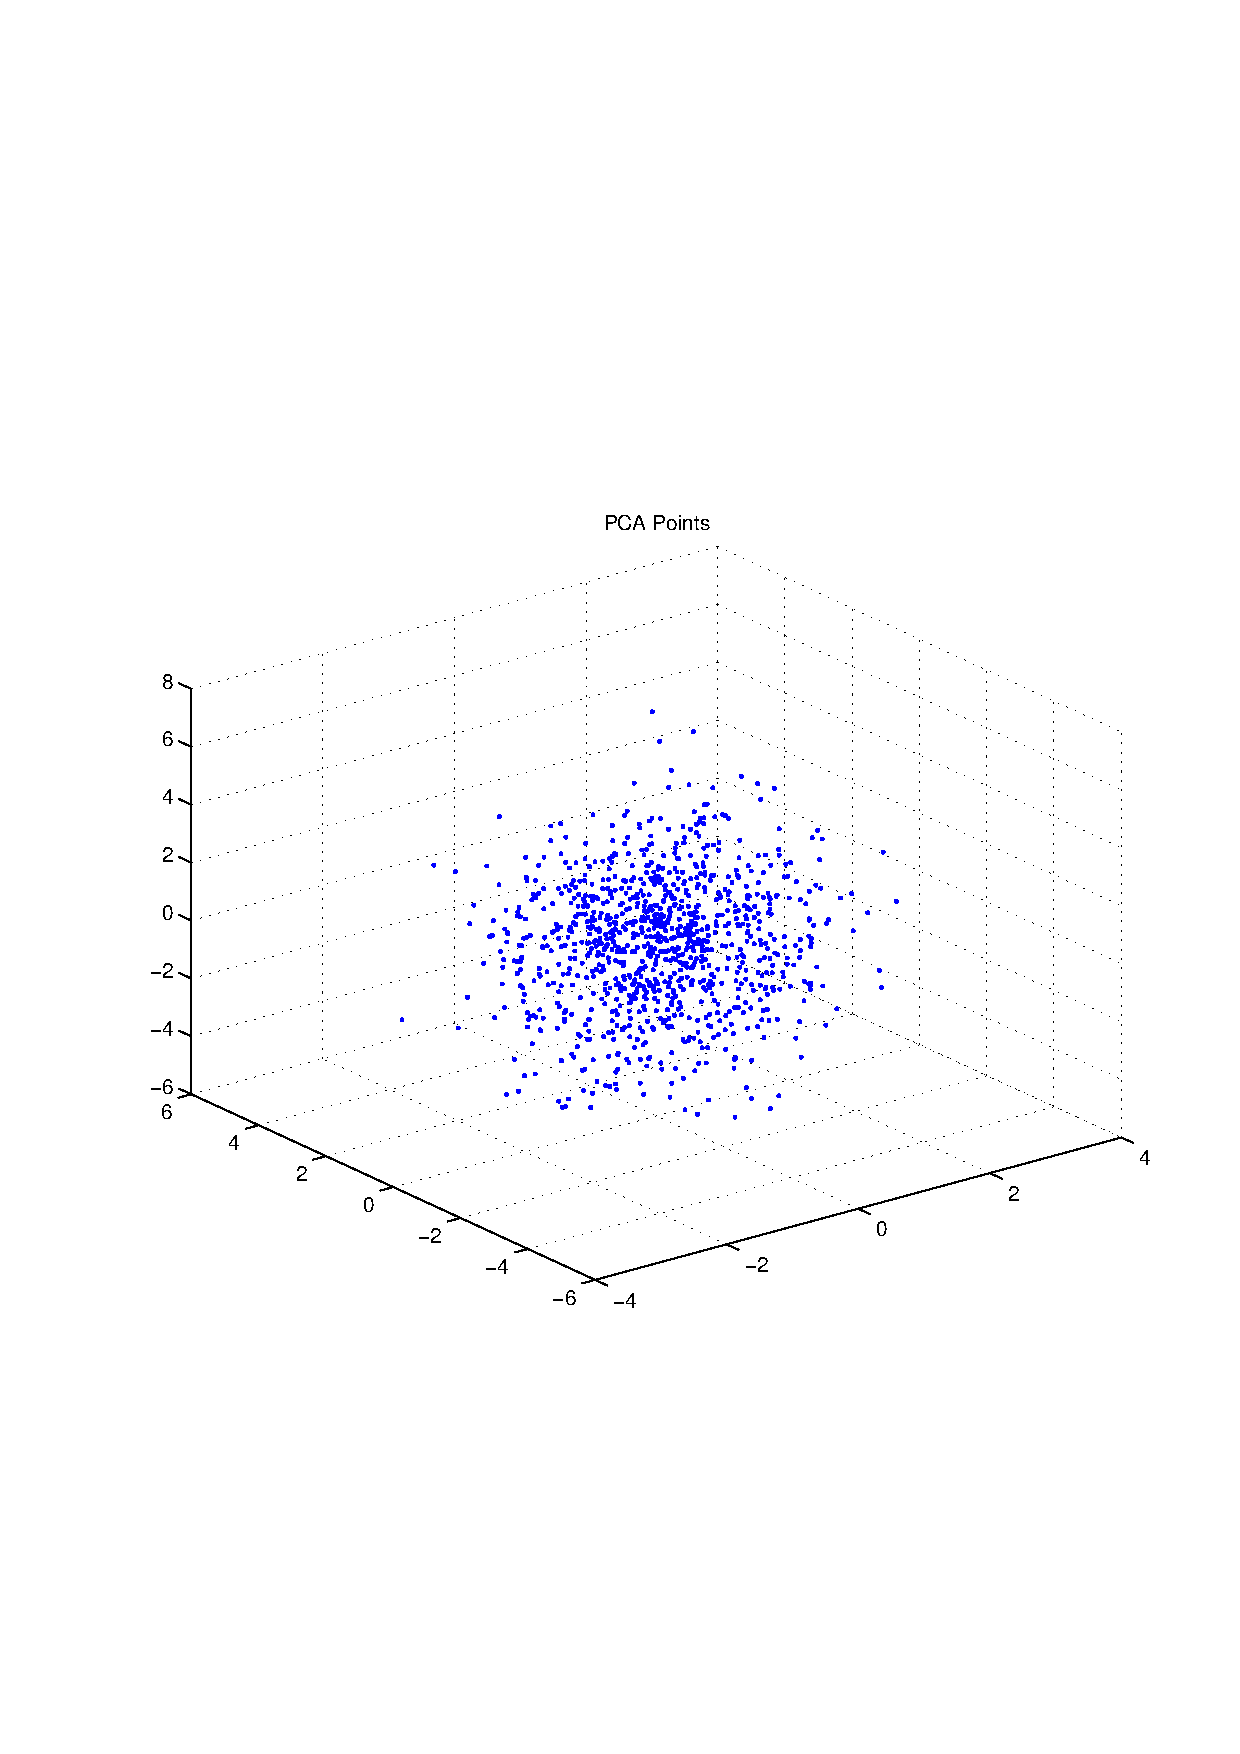
\includegraphics[width=10.0cm,height=10.0cm]{PCAPoints.pdf}

The eigenvectors:
+0.078, -0.004, +0.997
+0.111, +0.994, -0.005
-0.991, +0.111, +0.078

All of the eigenvalues of the covariance matrix:
(+0.958,+0.000), (+2.025,+0.000), (+3.017,+0.000)

QueryPerformanceCounter  =  +1.165
\subsubsection{Multi Variate Random Number Generator }
Sample from $N(\mu,\Sigma)$
mean= -0.002, variance=+1.004, skewness=+0.006, kurtosis=+3.003
mean= -0.001, variance=+1.017, skewness=-0.005, kurtosis=+2.988
mean= -0.002, variance=+1.006, skewness=-0.016, kurtosis=+3.014
Covariance Matrix 
+1.004, +0.009, +0.003
+0.009, +1.017, -0.003
+0.003, -0.003, +1.006

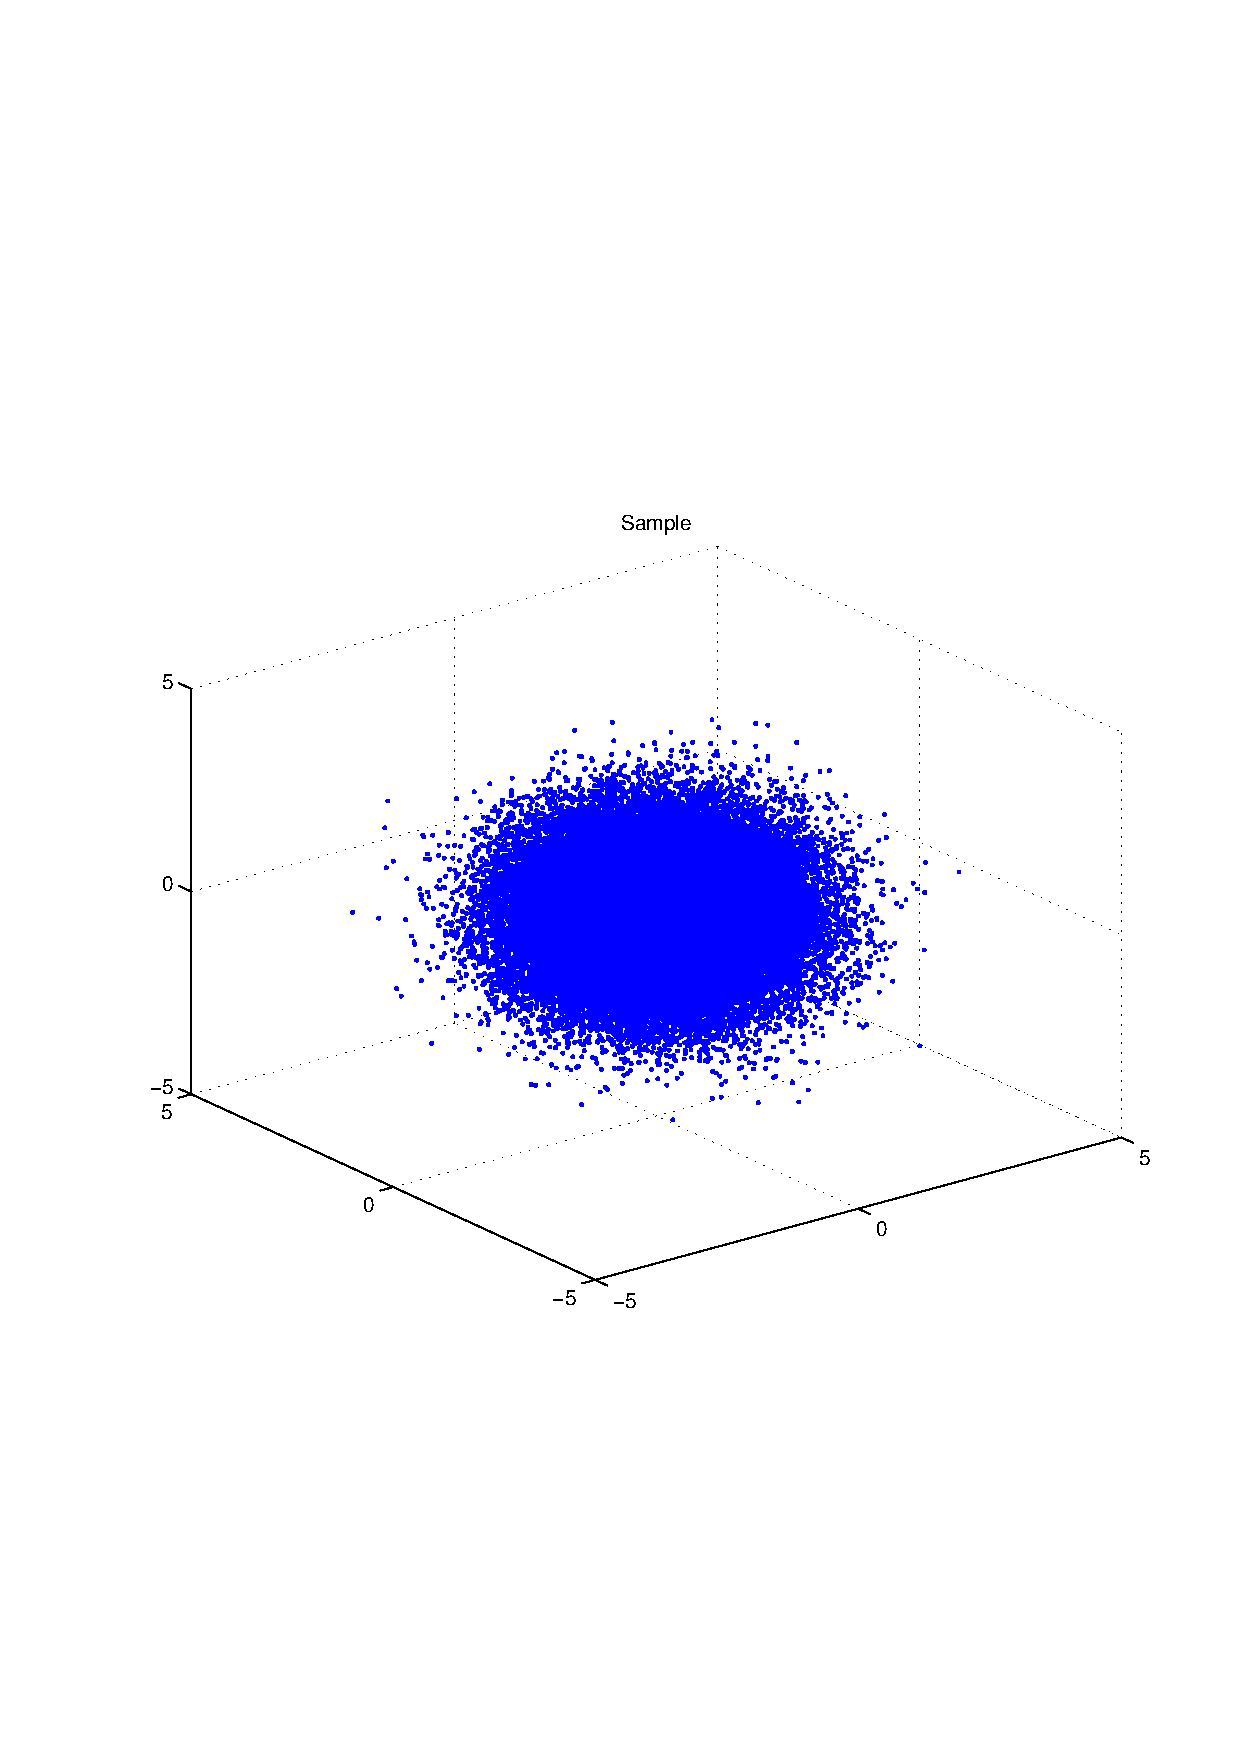
\includegraphics[width=10.0cm,height=10.0cm]{R_3_Normal.pdf}

Generate a sample from a unifom mixture of three Gaussians in $R^3$
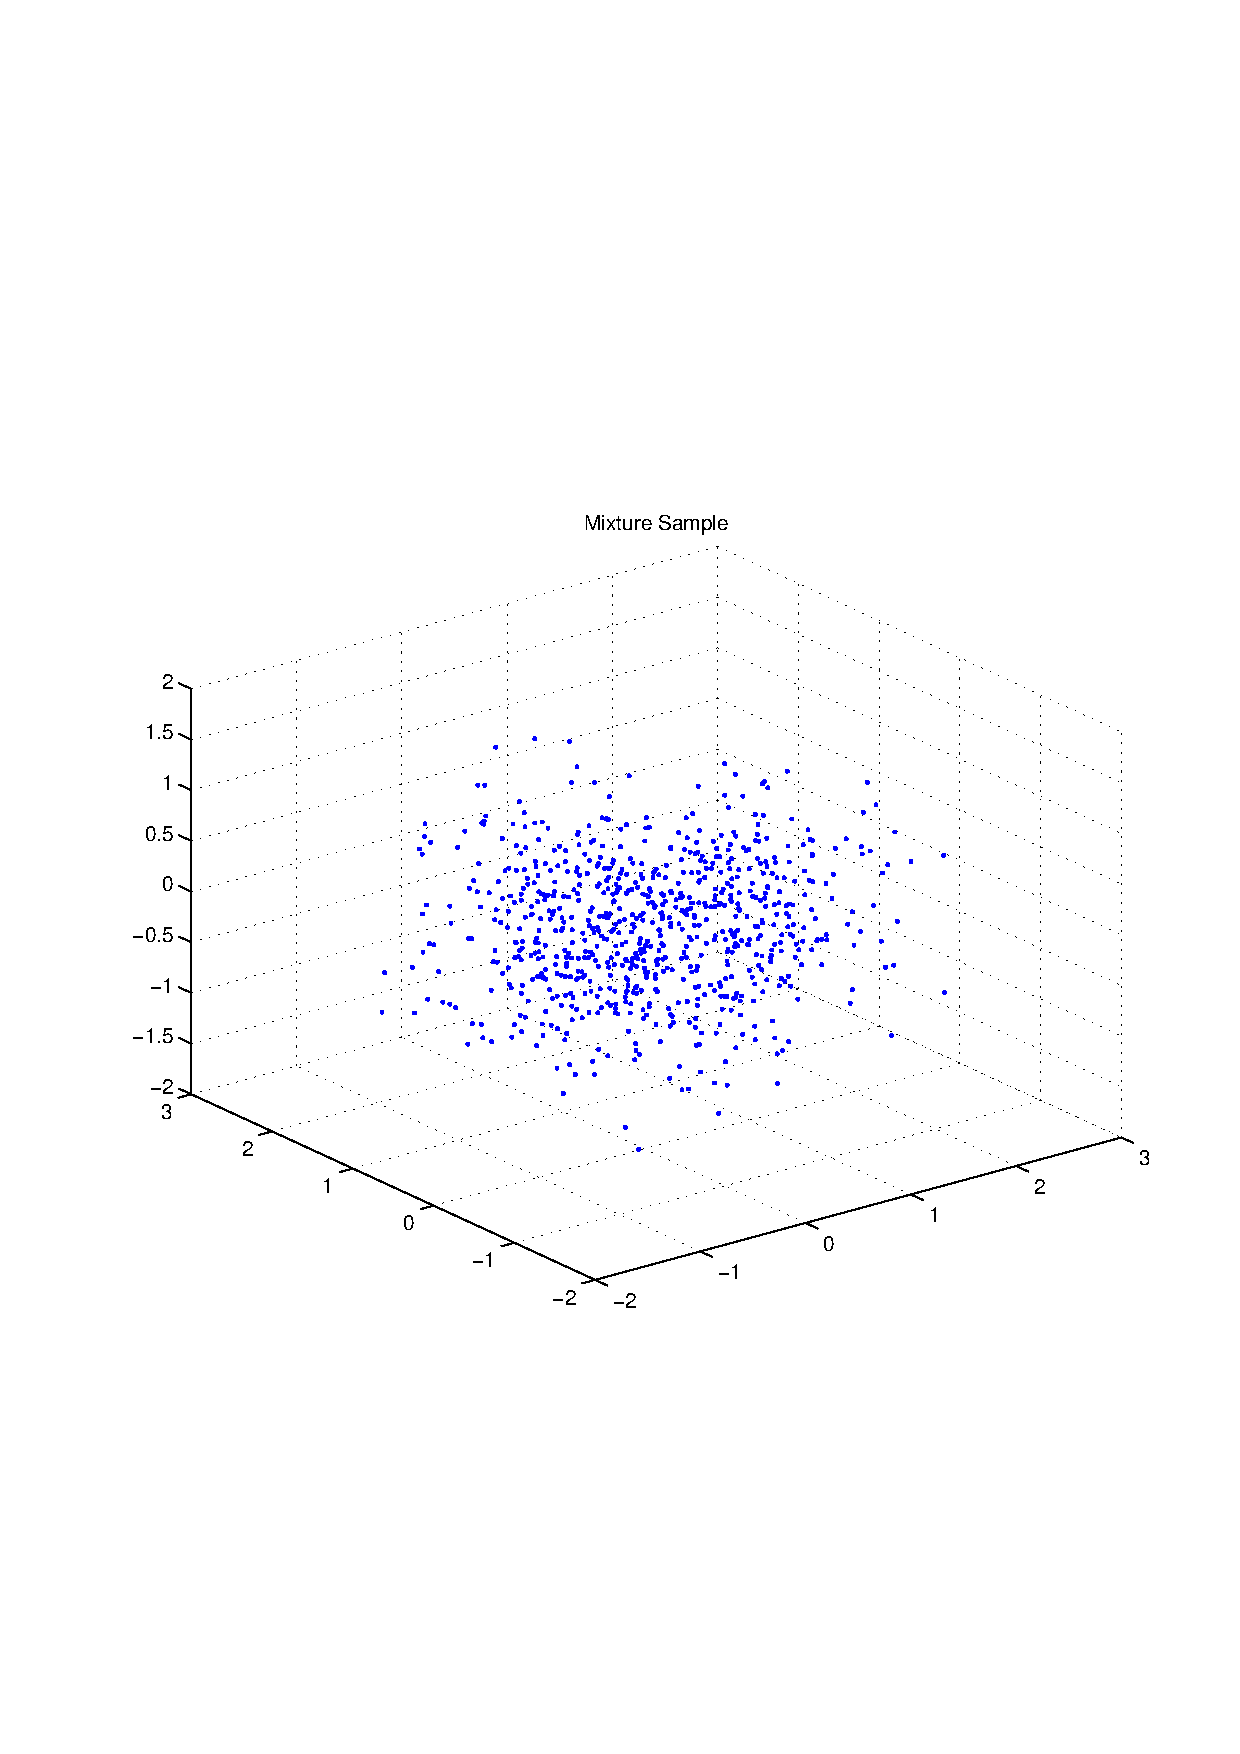
\includegraphics[width=10.0cm,height=10.0cm]{R_3_Normal_Mixture.pdf}

QueryPerformanceCounter  =  +13.999
\subsubsection{Matrix Multiply}
Comparing naive matrix multiply verus Intel MKL dgemm for matrix of size 2048.
This is for type double (hence the d in dgemm).
Naive type double matrix multiply tic toc  =  +0.360
dgemm plus row to column major transpose operation tic toc  =  +0.291
Comparing naive matrix multiply verus Intel MKL sgemm for matrix of size 2048.
This is for type float (hence the s in dgemm).
Naive type float matrix multiply tic toc  =  +0.220
sgemm plus row to column major transpose operation tic toc  =  +0.164
QueryPerformanceCounter  =  +1.120
\subsubsection{Descriptive Statistics}
Mean N(0,1): +0.003
Variance N(0,1): +1.006
Mean N(0,1) [recurrence relation method] :+0.003
Variance [recurrence relation method] :+1.006
Skewness : +0.007
Kurtosis : +2.997
QueryPerformanceCounter  =  +0.020
\subsubsection{Time Series }
+0.093
+0.726
+0.011
+2.178
QueryPerformanceCounter  =  +0.065
\subsubsection{Matrix}
QueryPerformanceCounter  =  +0.008
QueryPerformanceCounter  =  +0.008
\end{document}
